\documentclass[11pt,regno]{amsart}
%\setlength{\hoffset}{-.5in}
\setlength{\voffset}{-.25in}
\usepackage{amssymb,latexsym}
\usepackage{lscape}
\usepackage{acronym}
\usepackage{graphicx}
\usepackage{url}		%does nice formatting of URLs
\usepackage{amsfonts,amsmath,amssymb,amsthm}
\usepackage{bm,nicefrac}
\usepackage{siunitx}
\usepackage{derivative}
\usepackage{amsmath,amssymb}
\usepackage{setspace}
\usepackage{csquotes}
\usepackage{caption}
\newacro{Federal Reserve Economic Data}

\DeclareMathOperator{\EX}{\mathbb{E}}% expected value

\textwidth=6.175in
\textheight=9.0in
\headheight=13pt
\calclayout



\newcommand{\R}{{\mathbb R}}
\newcommand{\t}{{\texttt}}
\newcommand{\Q}{{\mathbb Q}}
\newcommand{\C}{{\mathbb C}}
\newcommand{\N}{{\mathbb N}}
\newcommand{\Z}{{\mathbb Z}}

\theoremstyle{plain}
\numberwithin{equation}{section}
\newtheorem{thm}{Theorem}[section]
\newtheorem{theorem}[thm]{Theorem}
\newtheorem{lemma}[thm]{Lemma}
\newtheorem{example}[thm]{Example}
\newtheorem{definition}[thm]{Definition}
\newtheorem{proposition}[thm]{Proposition}

\newcommand{\helv}{%
  \fontfamily{phv}\fontseries{m}\fontsize{9}{11}\selectfont}

\begin{document}
%% replace the values in the next three lines by the correct information
\setcounter{page}{1}

\title{}
\author{}
\thispagestyle{plain}
\begin{center}
    \Large
    \textbf{Analyzing the Russo-Ukrainian War's Effect On The World Economy}
        
    \vspace{0.4cm}
    \large
    \textbf{David Nieves Acarón \& Sam Sharp}
        
    \vspace{0.4cm}
    \textbf{MTH-5324}
    
    \vspace{0.4cm}
    \textbf{Dr. Nezamoddin N. Kachouie}

    \vspace{0.4cm}
    \textbf{Spring 2023}
\end{center}
\email{dnievesacaro2018@my.fit.edu csharp2021@my.fit.edu}
\thanks{}








\maketitle % generates the title of the paper 
\doublespacing 


% \textbf{\section{ Abstract }}
\section{ Abstract }

In this project we explore the effects of the Russo-Ukrainian war on the economies of the United States, Japan, the People's Republic of China, and the European Union, primarily through analysis of their respective Gross Domestic Product and national currency values. Three distinct methods are used for our analysis being multiple regression, generalized additive models, and autoregressive models. Through hypothesis testing for separate multiple regression models and forecasting over post-war data, we establish noticeable effects on the economies of these nations from the war. Additionally, similar results can be illustrated on relevant commodity prices associated with Russia and Ukraine.


\ 

\ 

\ 

\ 

\ 

\ 

\

\ 





\section*{Introduction}
The analysis of the economic impact of a war is just one way of assigning meaning to it. In this report, we are concerned with establishing a connection between a change in economic variables for the United States, China, the European Union, and Japan before and after the invasion of Ukraine in February of 2022. The events of late February 2022 shocked much of the world and resulted in large scale economic shifts. Almost immediately following the invasion, a cascade of economic turmoil entered financial markets across the globe while certain economies have begun to see higher inflation. Energy and food crises became household topics and many nations enacted economic sanctions against the Russian Federation.

Our goal is primarily to find a significant effect of the war on certain economies using statistical tests and forecasting methods. Multiple regression, generalized additive models, and autoregressive models are employed to achieve these ends with promising results to be expanded on.

For multiple regression, we construct a multitude of models and then conduct hypothesis tests on predictors to establish if there is a significant difference in the independent variable's estimate coefficients between the pre-war and post-war eras. Owing to their benefit with nonlinearity, generalized additive models (GAMs) are employed in an effort to fit models which can attempt to accurately forecast the GDP and currency evolution under models trained under pre-war datasets.


There is a multitude of statistical research papers analyzing the effects of war and other conflicts on economies and related variables. Glick and Taylor used statistical methods to measure the effects of war on trade between warring and neutral nations, with a conclusion that the economic welfare of such nations is significantly affected \cite{Glick} . Nations in Sub-Saharan Africa have been shown to have higher levels of civil conflict when experiencing negative economic growth \cite{subafrica}. Researchers at Harvard University have given support to the notion that civil wars can significantly effect economic growth, particularly with respect to private investment \cite{economic_civil_war}. Furthermore and related to our own look at GDP, a study from the European Bank for Reconstruction and Development establishes a significant drop in GDP by nations in a state of war and other nations not experiencing war on their own territory. Additionally, this study shows lasting effects on the labor force supply and capital stocks even after the affecting war has concluded \cite{european_bank}. These studies not only establish these negative relations with respect to warring nations, but also nations which take no part in the fighting itself, as seen by African nations not in civil conflict, or trade levels decreasing among nations not taking part in wars. This motivates our own research into the economic effects of the war in Ukraine on nations such as China, the United States, and Japan. While these nations are not fighting with troops on the ground, statistical analysis might still be able to show a significant difference on their economies in pre-war and post-war eras. 

Regarding our methods, the utilization of multiple regression is prevalent in such related studies. Book and Ekelöf use multiple linear regression techniques to establish the connection between the success of small businesses and certain macroeconomic factors \cite{macroeconomic_mult_linreg}. Stephen Bazen expands on the overwhelming utility of linear regression models for labor economics, showing that such models are extremely prevalent in an economic context \cite{linear_regression_economics}. Similarly, besides the use of multiple regression, other models will be considered due in part to the limitations associated with regression. First, there is no dearth of GAM related research regarding economics. Consider the study by S. Sapra which utilized multiple GAM models on business and economic datasets across a range of potential applications. This study expands on the potential advantage of a GAM against a standard multiple regression model in the case where there is an inadequate fit \cite{GAM_business}.  Additionally, for example, the use of autoregressive, time-series models with economic data is a well-established practice as seen in 
\cite{time_series_models}. In particular, ARIMA models as developed by \cite{ARIMA_original} are widely used in forecasting time-series data for economics and finance \cite{ARIMA_forecasting}, which is partially why they were chosen for this project. Moreover, combined with the use of exogeneous variables which change in time and also affect the response variables has been applied to several economics and business applications. For example, \cite{Thailand_ARIMAX} attempt to use ARIMAX to model Thailand's exports to her trade partners, \cite{US-China-ARIMAX} attempts to model the monthly average of Brent crude oil price with the influence of the US-China trade war, and  \cite{irish-civil-war-ARIMAX} attempt to model suicide rates during and after the Irish Civil War. 

In sum, we see that Multiple Regression, Autoregression, and GAMS could be effectively utilized to measure the effects of the Russo-Ukrainian war on the world economy.

% first half is motivations about what we want to achieve
% literature review that supports what we have done 
% 

 

\section*{Data}

Our data is gathered from a wide variety of sources. Primarily, these involve FRED, Eurostat (the European Union's Statistics Directourate-General), the People's Bank of China, and the Bank of Japan. For each nation, we constructed a dataset comprising quarterly Gross Domestic Product (real or gross as specified further), Interest Rates (from their respective central bank), unemployment rate, government spending, the consumer price index (CPI), and the national currency for each respective nation. Our dataset is on a monthly time frame, and as such, in instances where quarterly data was gathered, linear interpolation was used to augment the data into months. For all data regarding currencies, only Close prices are used. 

Each nation's dataset is split into a pre-war dataset and post-war dataset for hypothesis testing and forecasting uses that will be discussed in the methods section. For the European Union, Japan, and the United States, the pre-war dataset consists of 121 individual months of data ranging from January 2012 to January 2022, while the post-war dataset consists of 14 months from February 2022 to April of 2023. The Chinese dataset is considerably shorter, with the pre-war dataset consisting of 47 months which ranges from August of 2018 to January of 2022, and the post-war dataset the same 14 months as the latter three. 


% ordered by table order

%######################################3
% USA 
%######################################3
First, for the United States, the CPI is for all consumer items for all wage earners in the United States as listed by the OECD on a quarterly basis. The interest rate data is the Federal Funds Rate given by the Federal Reserve of the United States. The government spending data is as percentage of the deficit (or surplus) relative to the gross GDP of the United States. The GDP is gross, not seasonally adjusted, given on a quarterly basis. The unemployment rate is a percentage representing the unemployed percentage of the available labor force. The currency dollar is the U.S. Dollar Index, which is a relative metric which gauges the value of the U.S. dollar relative to European Union, Swiss Franc, Japanese Yen, Canadian Dollar, British Pound, and Swedish Krona.


%######################################3
% Europe 
%######################################3

For the European Union's CPI, all items were considered for all countries in the Euro area (19 countries in total) as seen in our accompanying source. The interest rate data for the European Union is the European Central Bank's Main Refinancing Operation Rate under Fixed Rate tenders. This was chosen as an analogue to the Federal Reserve's Federal Funds Rate. For government spending, the data used involved the 19 country area as seen in the accompanying Eurostat source. Its units are in percentages and they are listed from 2013 to 2022 in a yearly basis. Similarly for unemployment rates, the 19 country zone unemployment in units of percentages was used. The granularity of this data is in months, ranging from 1990 to January of 2023. Finally, the Euro's performance was obtained from Yahoo Finance's Python API using the ticker symbol of "EURUSD=X", with it being measured relative to the U.S. dollar.

%######################################3
% China 
%######################################3

The PRC's data was the most burdensome to obtain as many of the data is listed in a yearly basis. The CPI is in units in 2015 indices in a quarterly granularity, with the dates ranging from 1993 to 2022 given as under all items by the OECD. The government spending is a percentage of the deficit relative to China's GDP that quarter. The GDP is the Real GDP (relative to 2017 U.S. dollars) given yearly. The interest rate used is the Chinese 1 year Loan Prime Rate from the People's Bank of China.  The interest rates were obtained from an intermediary source which in turn gets the data from our attached primary source. They are in units of percentages and are in yearly granularities.  The unemployment rate is also in percentages in a yearly granularity measured as the percentage of the labor force which is unemployed. Similarly, the currency data corresponds to the USD/CNY pairing with symbol "CNY=X" from Yahoo Finance. 

%######################################3
% Japan 
%######################################3


The CPI for Japan is with respect to All Items of 2015 indices, with a quarterly granularity from 1960 to the first quarter of 2022.  The interest rate is in the form of monthly units of percentages, with ranges from 1960 to February of 2023. This interest rate is the immediate 24 hour lending rate set by the Bank of Japan. For government spending, this is taken as a percent of government expenditure relative to GDP in yearly time ranges from 1970 to 2021. The GDP is quarterly, tied to the value of the Yen in 2015. The unemployment rate for Japan is a percentage of the unemployed populace ages 15 to 64, listed quarterly. Finally, the currency is the Japanese Yen relative to the Dollar, taken as the value at the end of each month.

The commodity data is the daily closing price for the following futures: Natural Gas (NY Mercantile), Wheat(CBOT Chicago), Crude Oil (NY Mercantile), and Soybean Oil (CBOT Chicago). Prices are valued in Dollars.

Please see Tables 1-5 in the supplementary report file for the sources for each respective data entry in the References section.


A combination of R scripts and Python scripts were used to aggregate the data. The use of an advanced text editor known as Vim was also of great value for quickly editing CSV files. The greatest issue we had was in aggregating data with different date formats. Some examples of these scripts used for this purpose include \texttt{main.py} \texttt{commod\.ipynb}, and    \texttt{change\_date\_format.py}.







\section*{Methods}

%##############################
% Multipel Regression- models standard, differenced, rlm
% T tests
% GAMS
% Robust Regression
% Autoregressive models 
% ARIMAX
% ARIMA
% 

We begin with multiple regression. Various multiple regression models were utilized, with two separate dependent variables studied. The two dependent variables used for our multiple regression models were each nation's monthly GDP and their respective currencies. Primarily, our regression models encompass two separate forms. The first is the standard regression with a dependent variable and multiple independent variables. The second is a difference model, which takes the same structure as the standard regression model with the exception that every variable is now recomputed as the difference between the two most recent entries. As for deciding which independent variables to use for each nation's respective dataset, correlation matrices were used for both standard and difference models. An example of these correlation matrices can be seen in Figure 1 of the supplementary document. Furthermore, one extra multiple regression model was utilized, which is the case of Robust Linear Models (RLMs), using Huber loss and M-estimators. Iterated reweighted least squares is used to find an M-estimator, which is used to better handle the effect of outliers on regression, which in turn can help one overcome violations of the assumptions of linear regression. For further information on the theory of robust regression, see \cite{RobustRegression} and \cite{Huber}.

The main method as for ascertaining an effect post-invasion on the nations economies comes in the form of testing whether there is a significant difference in the regression slopes on our pre-war and post-war models. This comes in the form of the following hypothesis test:


\begin{equation} \tag{1}
 \begin{cases} 
      H_0: \beta_{i,post} - \beta_{i,pre} = 0 \\
      H_a:\beta_{i,post} - \beta_{i,pre} \neq 0 \\
   \end{cases}
\end{equation} 

Where $B_{i,pre}$ is the respective estimate coefficient for the independent variable on the pre-war model and $B_{i,post}$ is the respective estimate coefficient for the independent variable on the post-war model. To test this hypothesis, we calculate the test-statistic as:



\begin{equation} \tag{2}
t = \frac{\beta_{i,post}- \beta_{i,pre}}{\sqrt{s_{\beta_{i,post}}^2+s_{\beta_{i,pre}}^2}} \sim T(n_1 +n_2 -4)
\end{equation} 

Where $s$ represents the standard error for each pre-war and post-war $B_i$ respectively, and $T$ represents the T distribution. $n_1$ and $n_2$ are the the lengths of the pre-war and post-war datasets respectively. In the case of,


\begin{equation} \tag{3}
|t| > T_{n_1+n_2-4, \frac{\alpha}{2}}
\end{equation} 

We are able to reject the null hypothesis and establish some statistical difference between the way the independent variable has affected the response variable between the pre-war and post-war eras. For this research, we use a 95$\%$ confidence interval. These hypothesis tests are only conducted if a certain multiple regression model returns independent variables in the regression summary which are \textit{both} statistically significant. In this case, the hypothesis test is conducted. The equations (1) and (2) were introduced and established as good practice by \cite{correct_stats}, who denote this practice as well-defined and effective in a criminology journal.

Additionally, we utilize GAMs for further efforts of forecasting. Tables 3 through 6 show each GAM model and the independent variables it used. Note that we employ two separate methods for these GAMS, one being Generalized Cross Validation (GCV) and the other Restricted Maximum Likelihood (REML). While GCV is the default designation for GAMs, we have chose to also utilize REML methods based on research in the literature suggesting that GCV methods can be prone to under-smoothing \cite{GAM_wood}. Every independent variable is made a smooth term using thin plate splines. In the post-war GAM models, knots of three units are used to ensure convergence.

For the autoregressive models, some analysis of the data was performed to determine what the model parameters, $p,d$, and $q$ are. 

This was done by looking at the partial autocorrelation function, the Dickey-Fuller test \cite{Dickey-Fuller}, and the autocorrelation function, which can help to determine the coefficients for $p$, $d$, and $q$, respectively. The coefficients for $p$ were chosen by taking the \textit{most} significant partial autocorrelation lag value, regardless of whether it lied inside or outside of the confidence intervals. the autocorrelation lag term was chosen by taking the last lag for which the term was significant (i.e. outside of the confidence interval). With regards to ARIMAX, the exogeneous variables were chosen by using the indicators which were previously shown to be significant by the earlier tests.  For the $d$ term, an iterative Dickey-Fuller test was performed by performing differencing on the response data using the \texttt{diff} function in R until the p-value of the test was found to be less than 0.01. A forecast of the response was performed by using the \texttt{forecast} function in R. This was then plotted against the points that reflected the \textit{true} response values at the times after the war started in order to get a sense of how different the actual response values are when compared to the forecasted response values. This process was repeated for both the country GDP data along with the associated exogeneous variables indicated in each of the accompanying plots as well as the commodity data. To get a sense of how different the post-war and pre-war situations are and thus to possibly conclude that there is a significant difference, the use of the ARIMA $\&$ ARIMAX confidence intervals can be employed to see which of the predicted points lie outside of the 95\% confidence intervals (colored in light grey in the plots) of the ARIMA and ARIMAX forecasts. 

\section*{Results}
Table 1 lists each respective model for each nation's dataset and the independent variables used in the regression as dictated by the correlation matrices, as well as the pre-war and post-war respective models Adjusted R-squared value. Table 2 lists the independent variables which were significant in both pre-war and post-war models which then subsequently were able to reject the null hypothesis. Table 2 also lists each rejected predictors pre-war and post-war estimate coefficients, so one can see the change in how these variables effect the response from pre-war to post-war eras. The ARIMA forecasts superimposed over the post-war data for each commodity appears in Figure 1, where we can see the ARIMA models struggling to accurately forecast the events of the war. In Figures 2 and 3, the ARIMAX forecast is displayed for each nation over the post-war period. Figures 4 through 10 display each GAM forecast using GCV and REML methods for GDP and national currencies as responses. Correspondingly, Tables 3 through 6 show each GAM model with their respective Deviance Explained as a percentage.


\begin{figure}[h!]  
\caption*{\textit{Table 1:} Each nation's models and models and respective dependent and independent variables with the respective adjusted R-squared value for pre-war and post-war datasets..}
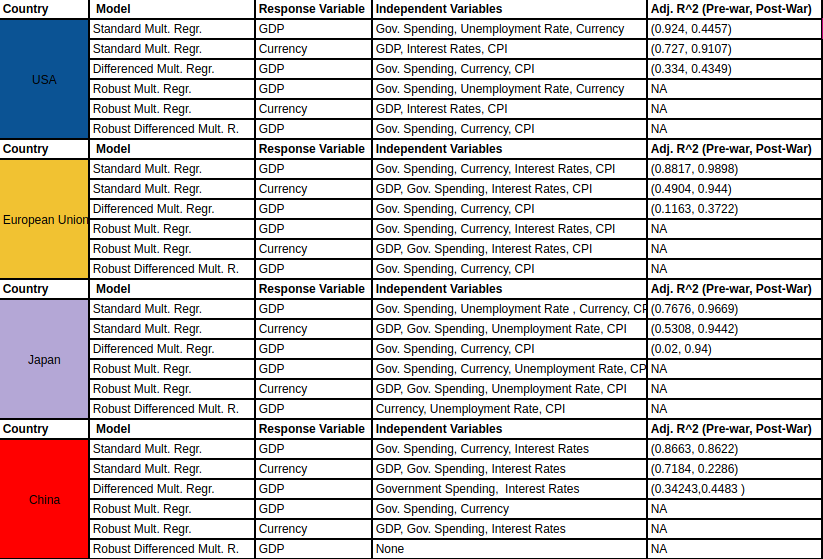
\includegraphics[scale = 0.4]{summary_table.png} 
\end{figure}

\begin{figure}
\centering
\centerline{ \mbox{
\subfigure{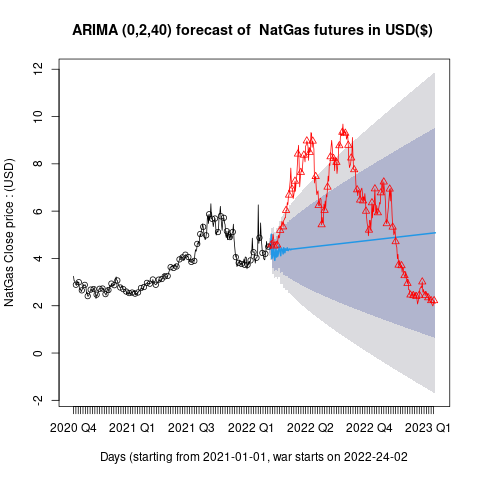
\includegraphics[width=2in]{ARIMA_NatGas.png}}  
\subfigure{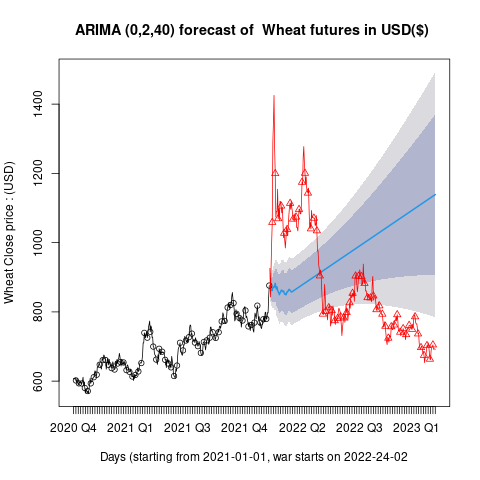
\includegraphics[width=2in]{ARIMA_wheat.png}}
\subfigure{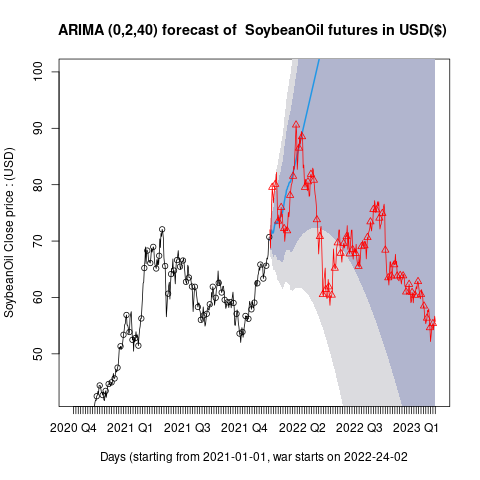
\includegraphics[width=2in]{ARIMA_SoybeanOil.png}}
\subfigure{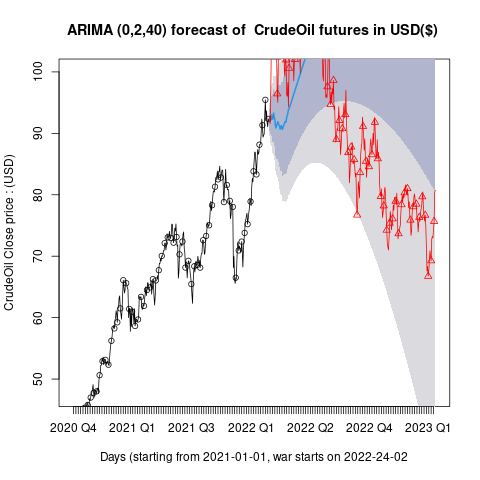
\includegraphics[width=2in]{ARIMA_CrudeOil.png}}
}}
\caption{Figures showing the ARIMA forecasts for two commodities: Natural Gas and Wheat futures. As can be shown particularly in the case of wheat, there is a significant deviation from the overall trend that is most likely a result of the beginning months of the war and the fact that Ukraine is the world's 5th largest exporter of wheat \cite{Wheat_Ukraine}.  }
\end{figure}

\begin{figure}[h!]  
\caption*{\textit{Table 2:} Table showing model types, rejecting predictors, and rejecting predictor estimates along with response variables for each nation}
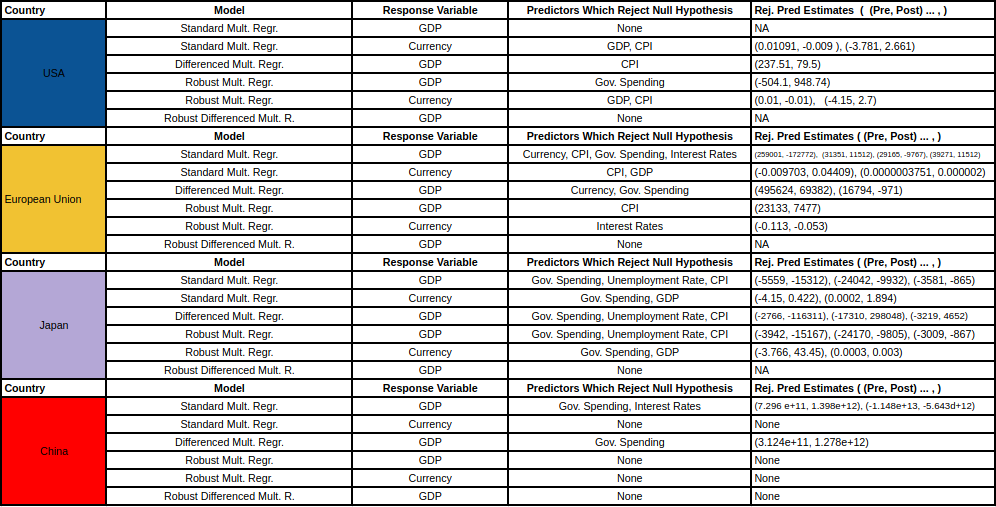
\includegraphics[scale = 0.5]{pred_rej_table.png} 
\end{figure}



% ARIMAX


\begin{figure}
\centering
\centerline{ \mbox{
\subfigure{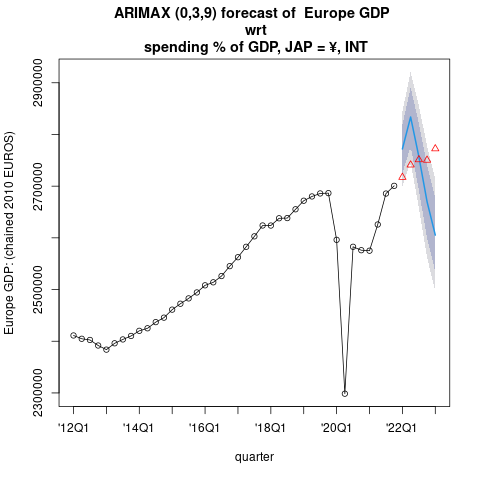
\includegraphics[width=2.5in]{ARIMA_EURO.png}}  
\subfigure{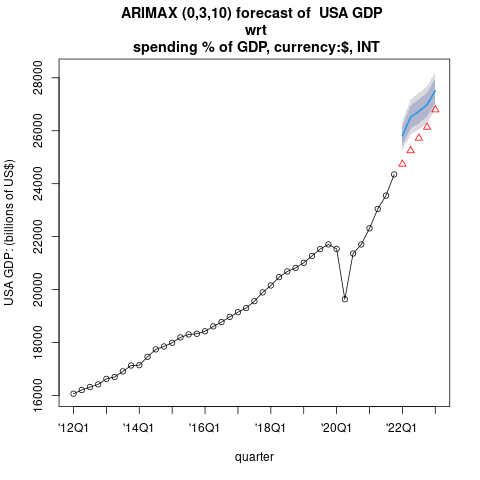
\includegraphics[width=2.5in]{ARIMA_USA.png}}
}}
\caption{ ARIMAX forecast for the European Union and USA GDP data. The EU data showcases a clear divergence from the trend established after the onset of the COVID fallout, whereas the USA data showcases a following of the trend, though in a capacity that is lower than what the prediction expects at the 95\% and 80\% confidence levels.}
\end{figure}

\begin{figure}
\centering
\centerline{ \mbox{
\subfigure{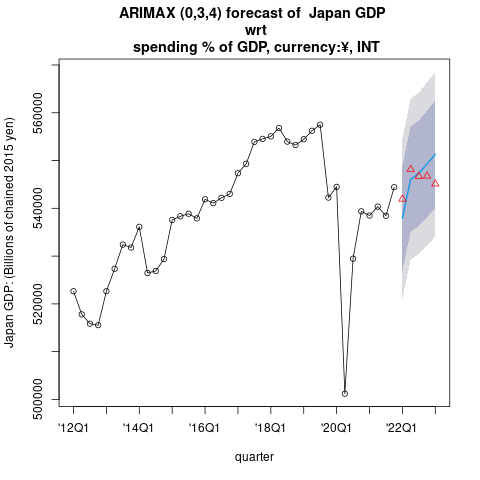
\includegraphics[width=2.5in]{ARIMA_JAPAN.png}}
\subfigure{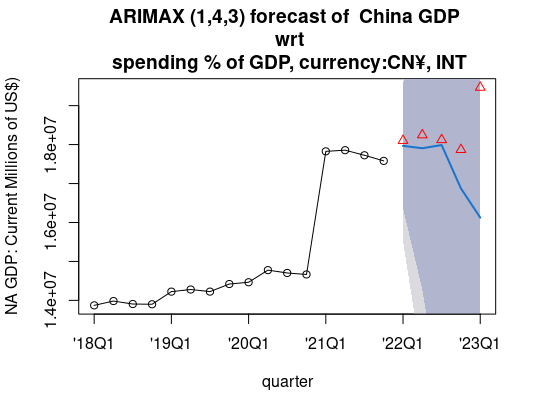
\includegraphics[width=2.5in]{ARIMA_China.png}}
}}
\caption{Plots showing the Japan and PRC predictions. For both, a large confidence interval is showcased. In the case of Japan, this could be explained by the war's relative distance (both physically and economically) from the island-nation. In the case of China, some faulty data has resulted in a confidence interval that is much too large to be interpretable. Overall, better method must be acquired and is being investigated.}
\end{figure}




%GAMSSSSS GAMS GAMS GAMS GAMS GAMS GAMSSSSSS

\begin{figure}
\centering
\centerline{ \mbox{
\subfigure{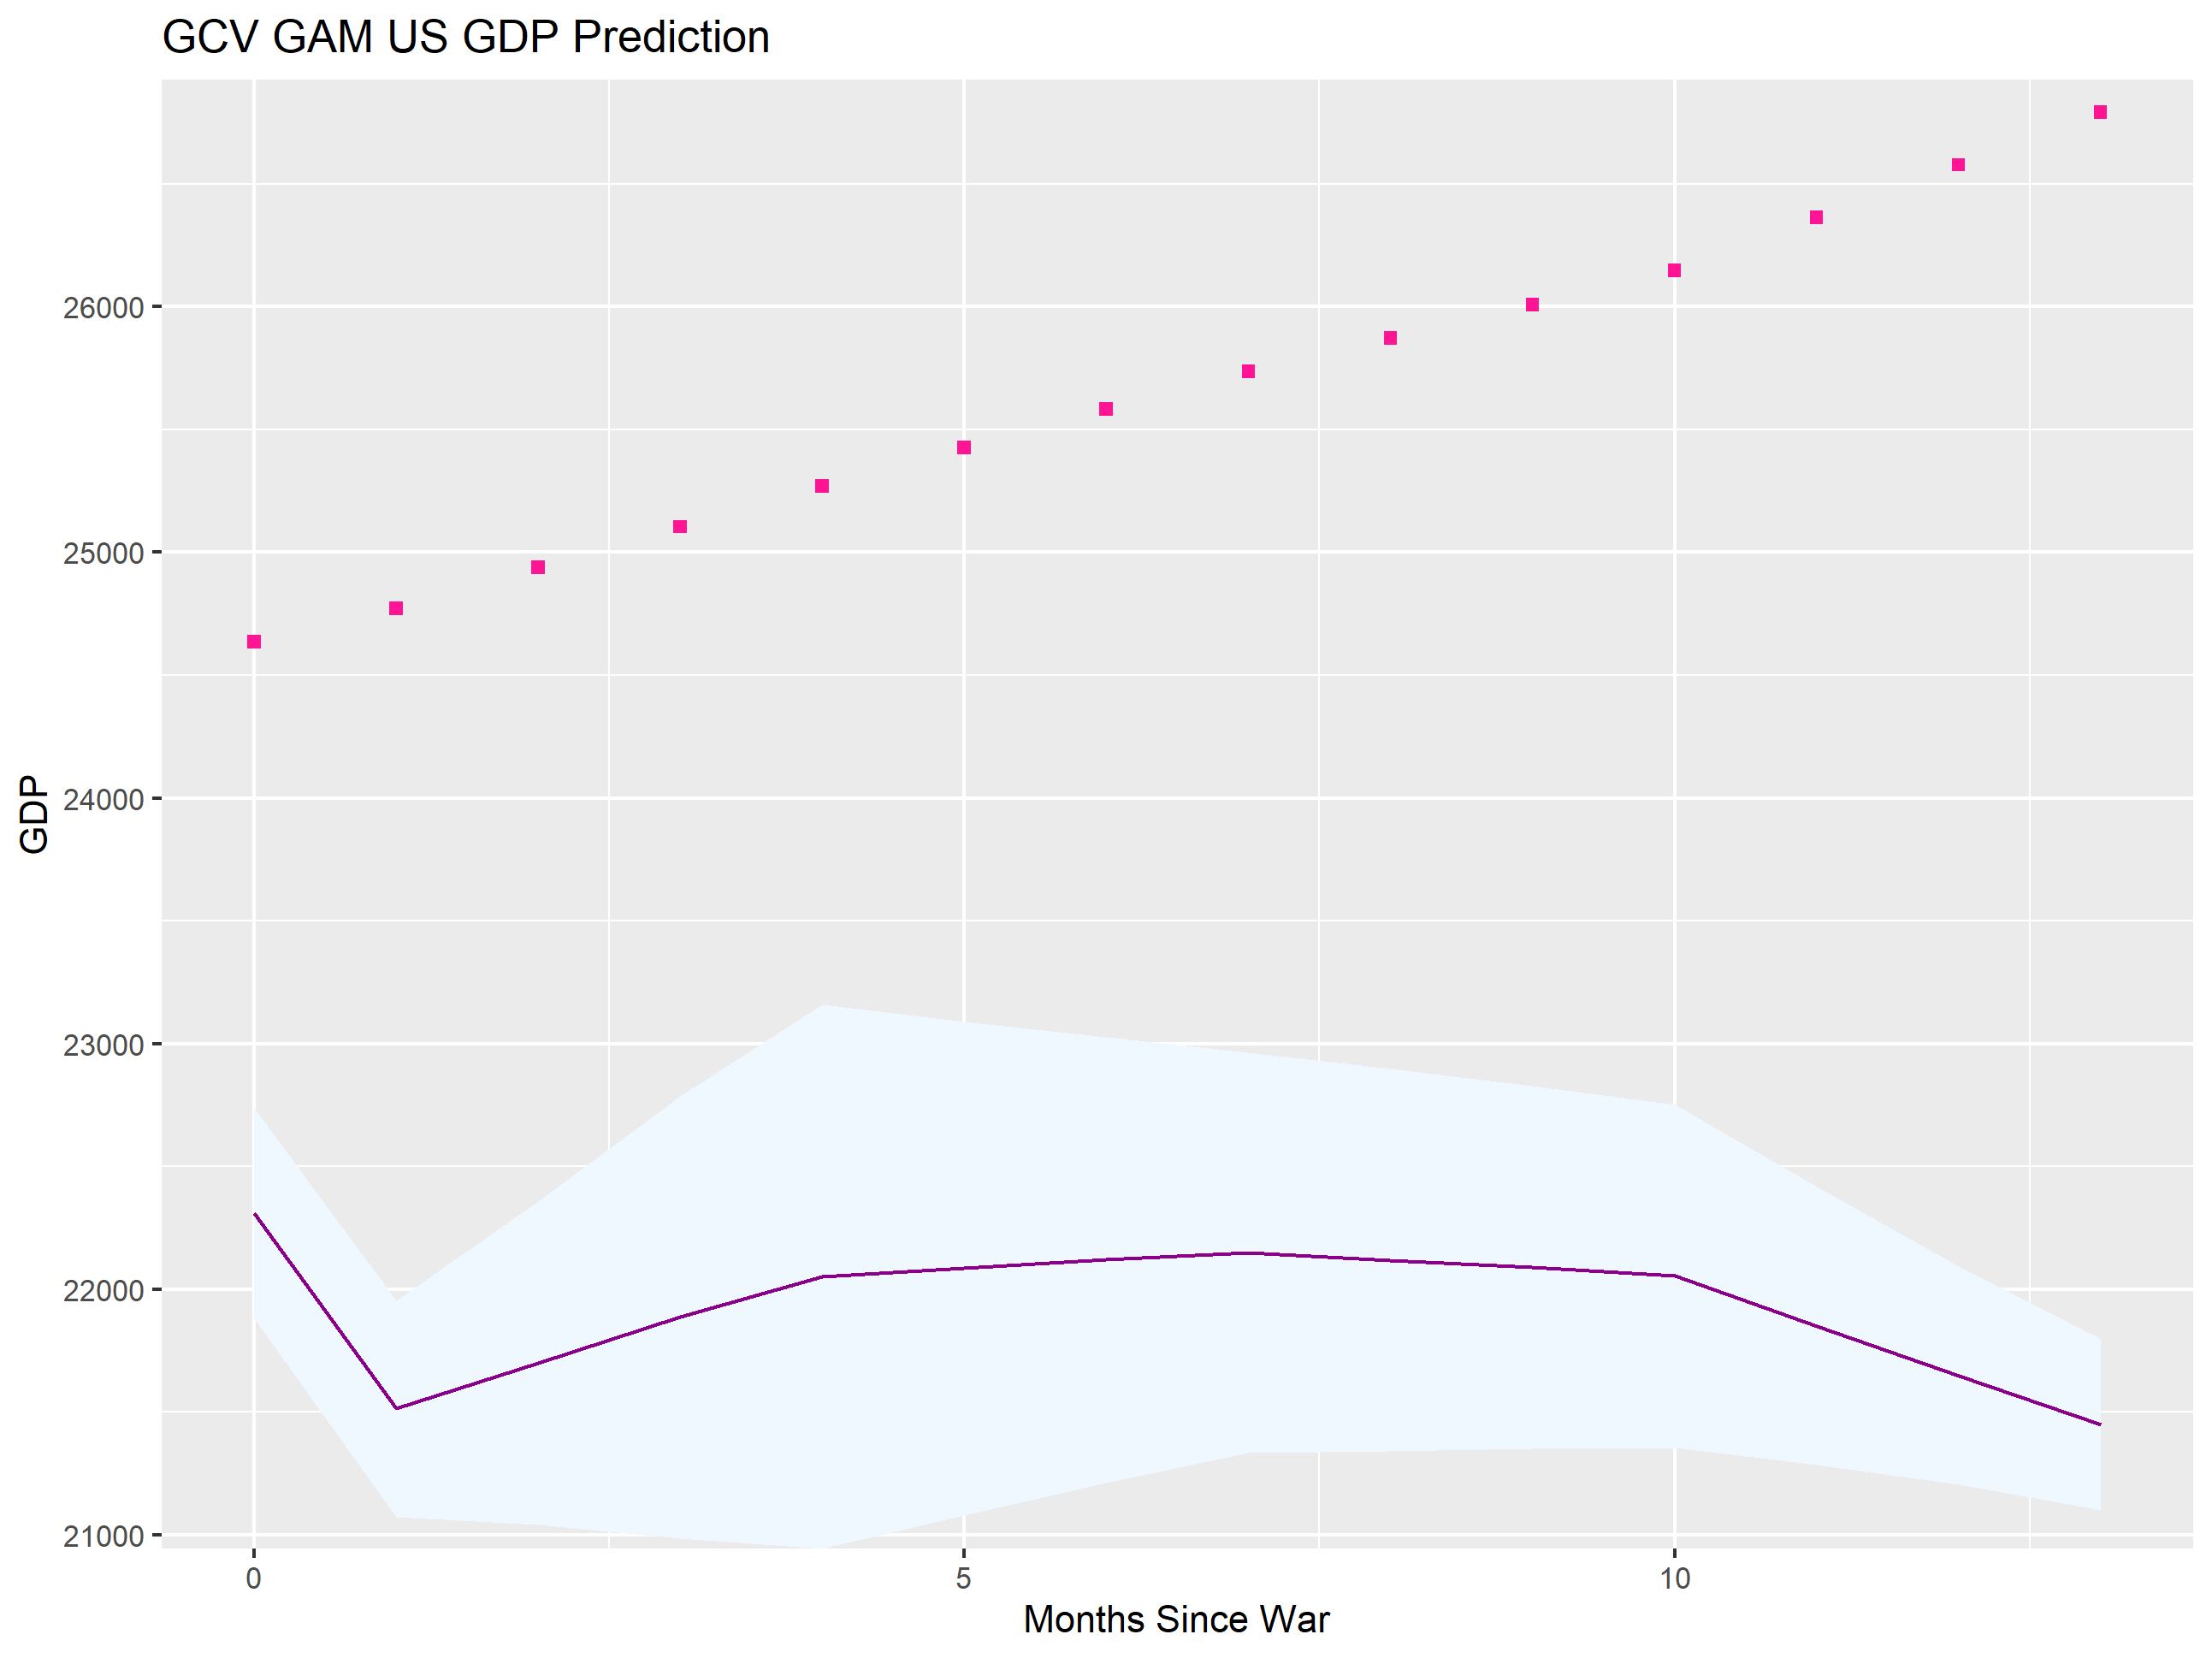
\includegraphics[width=2in]{report/us-gdp-gcv.png}}  
\subfigure{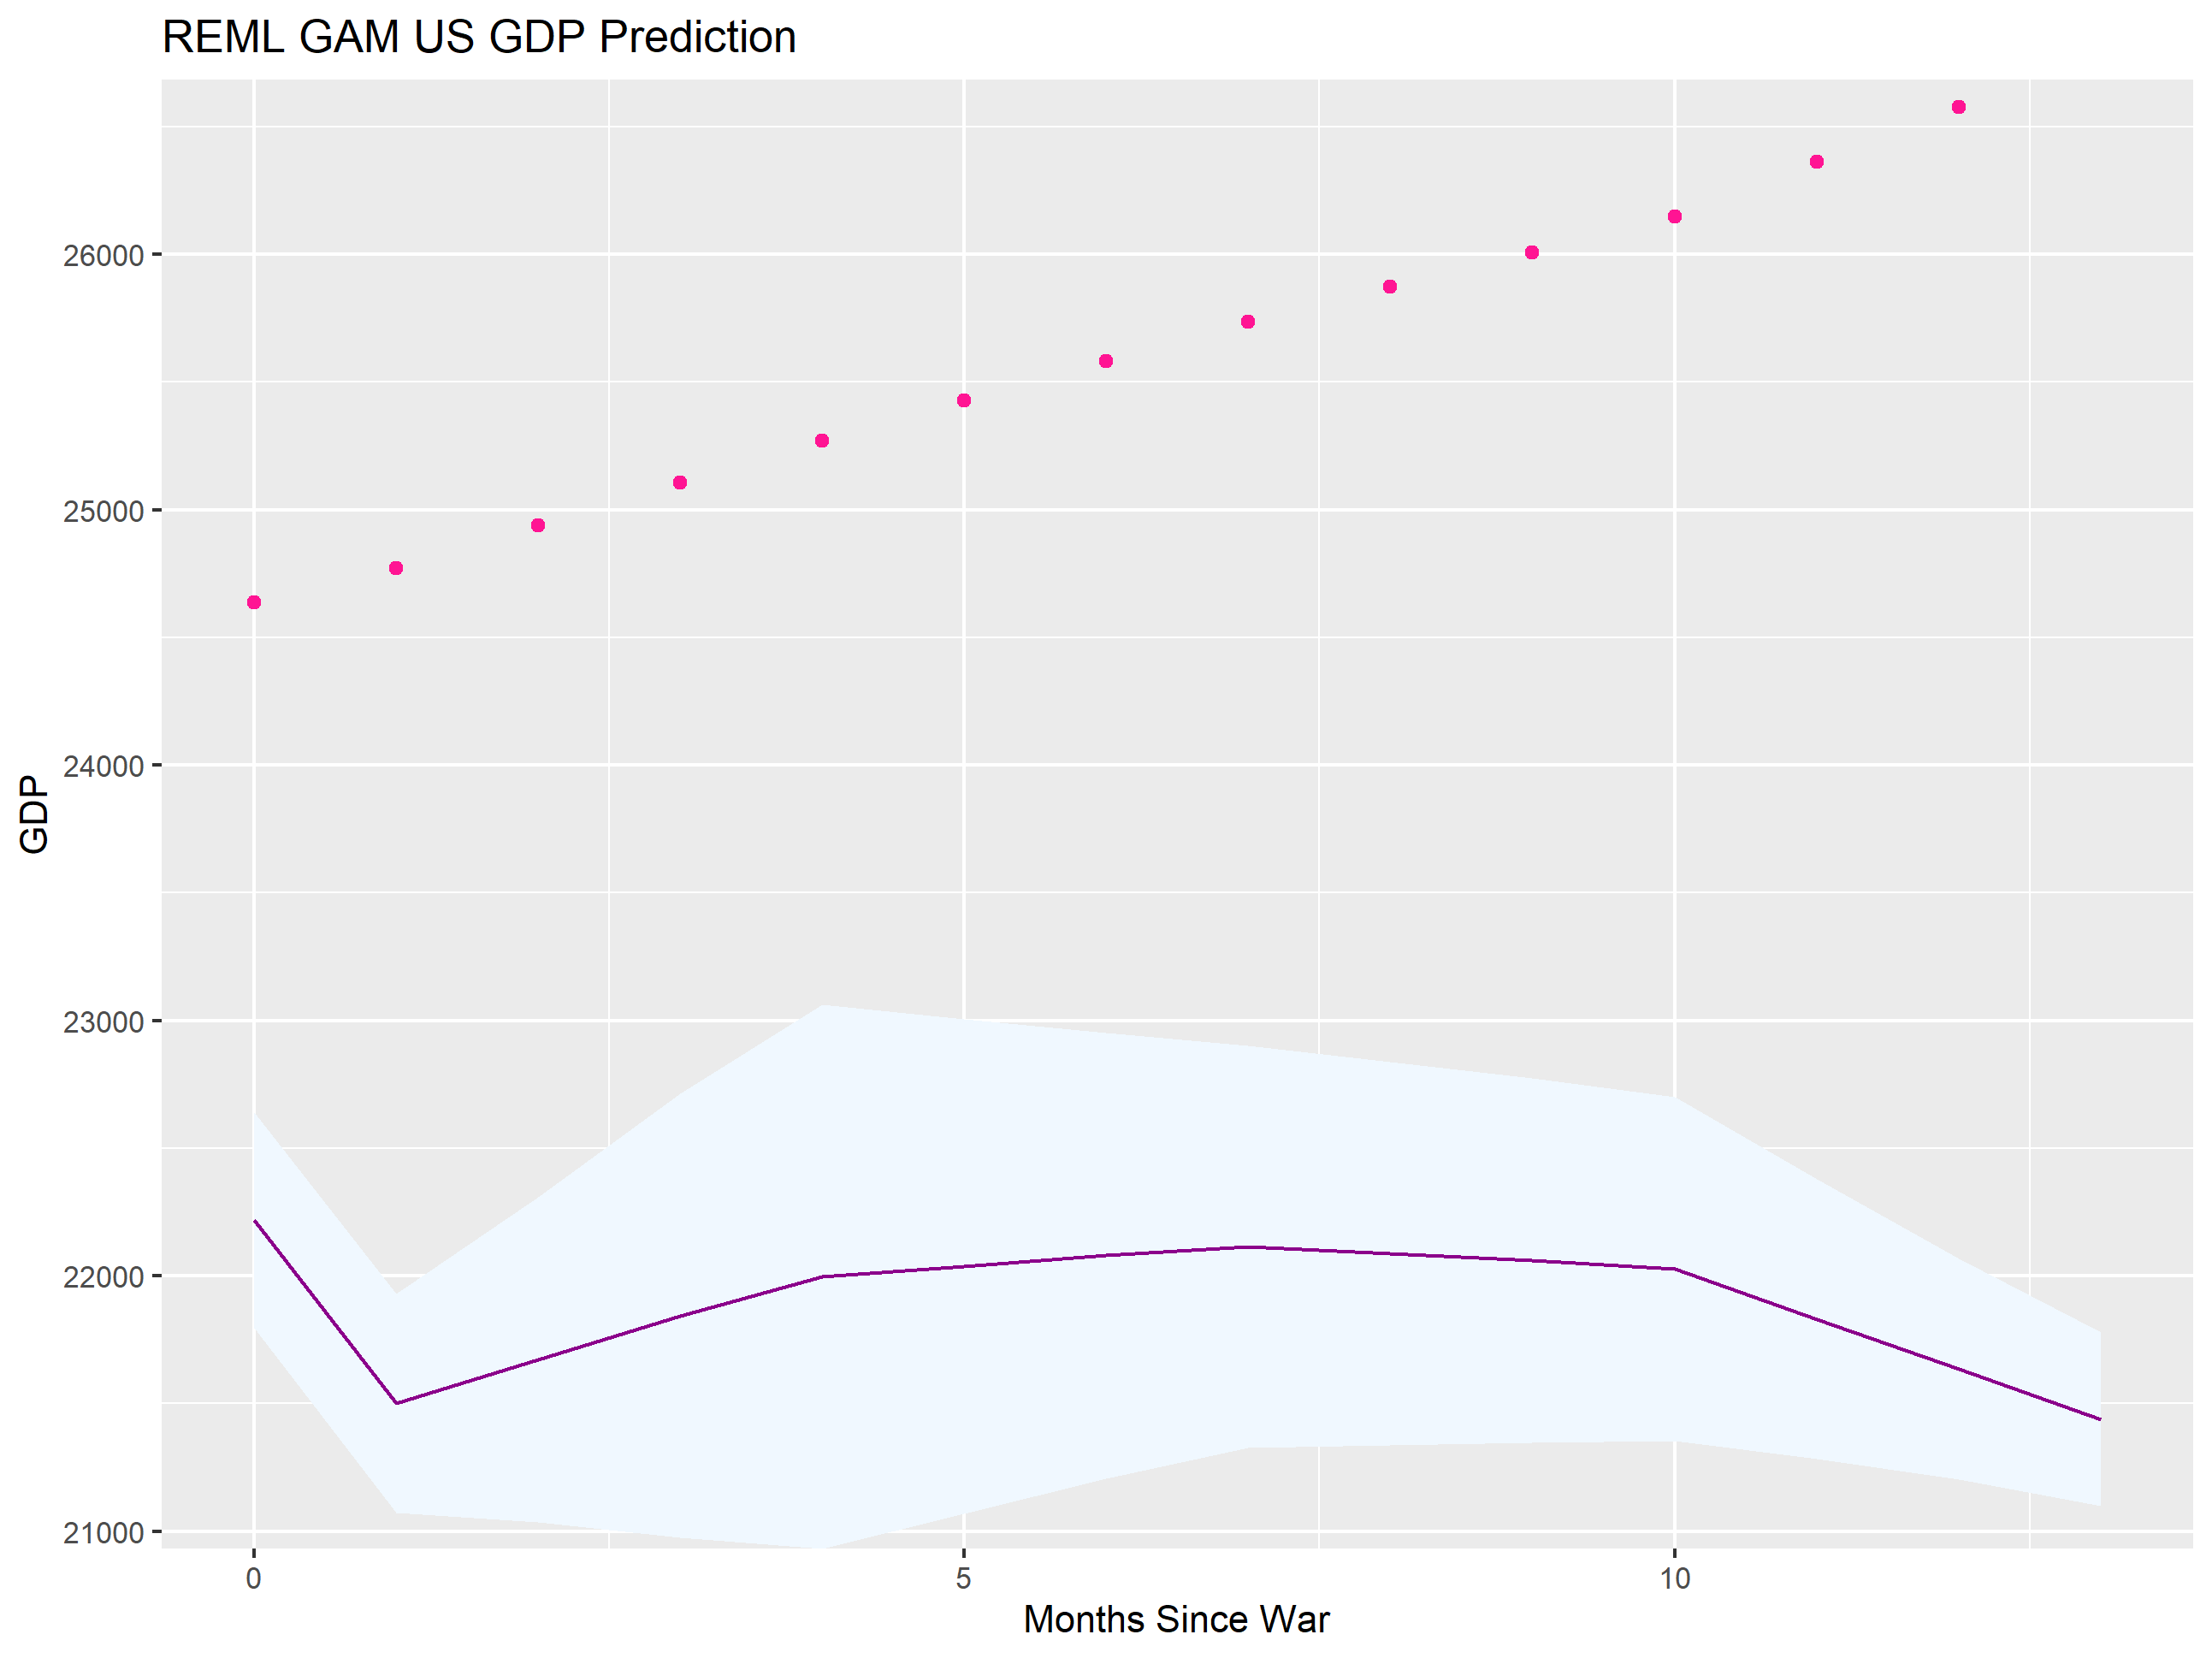
\includegraphics[width=2in]{report/us-gdp-reml.png}}
\subfigure{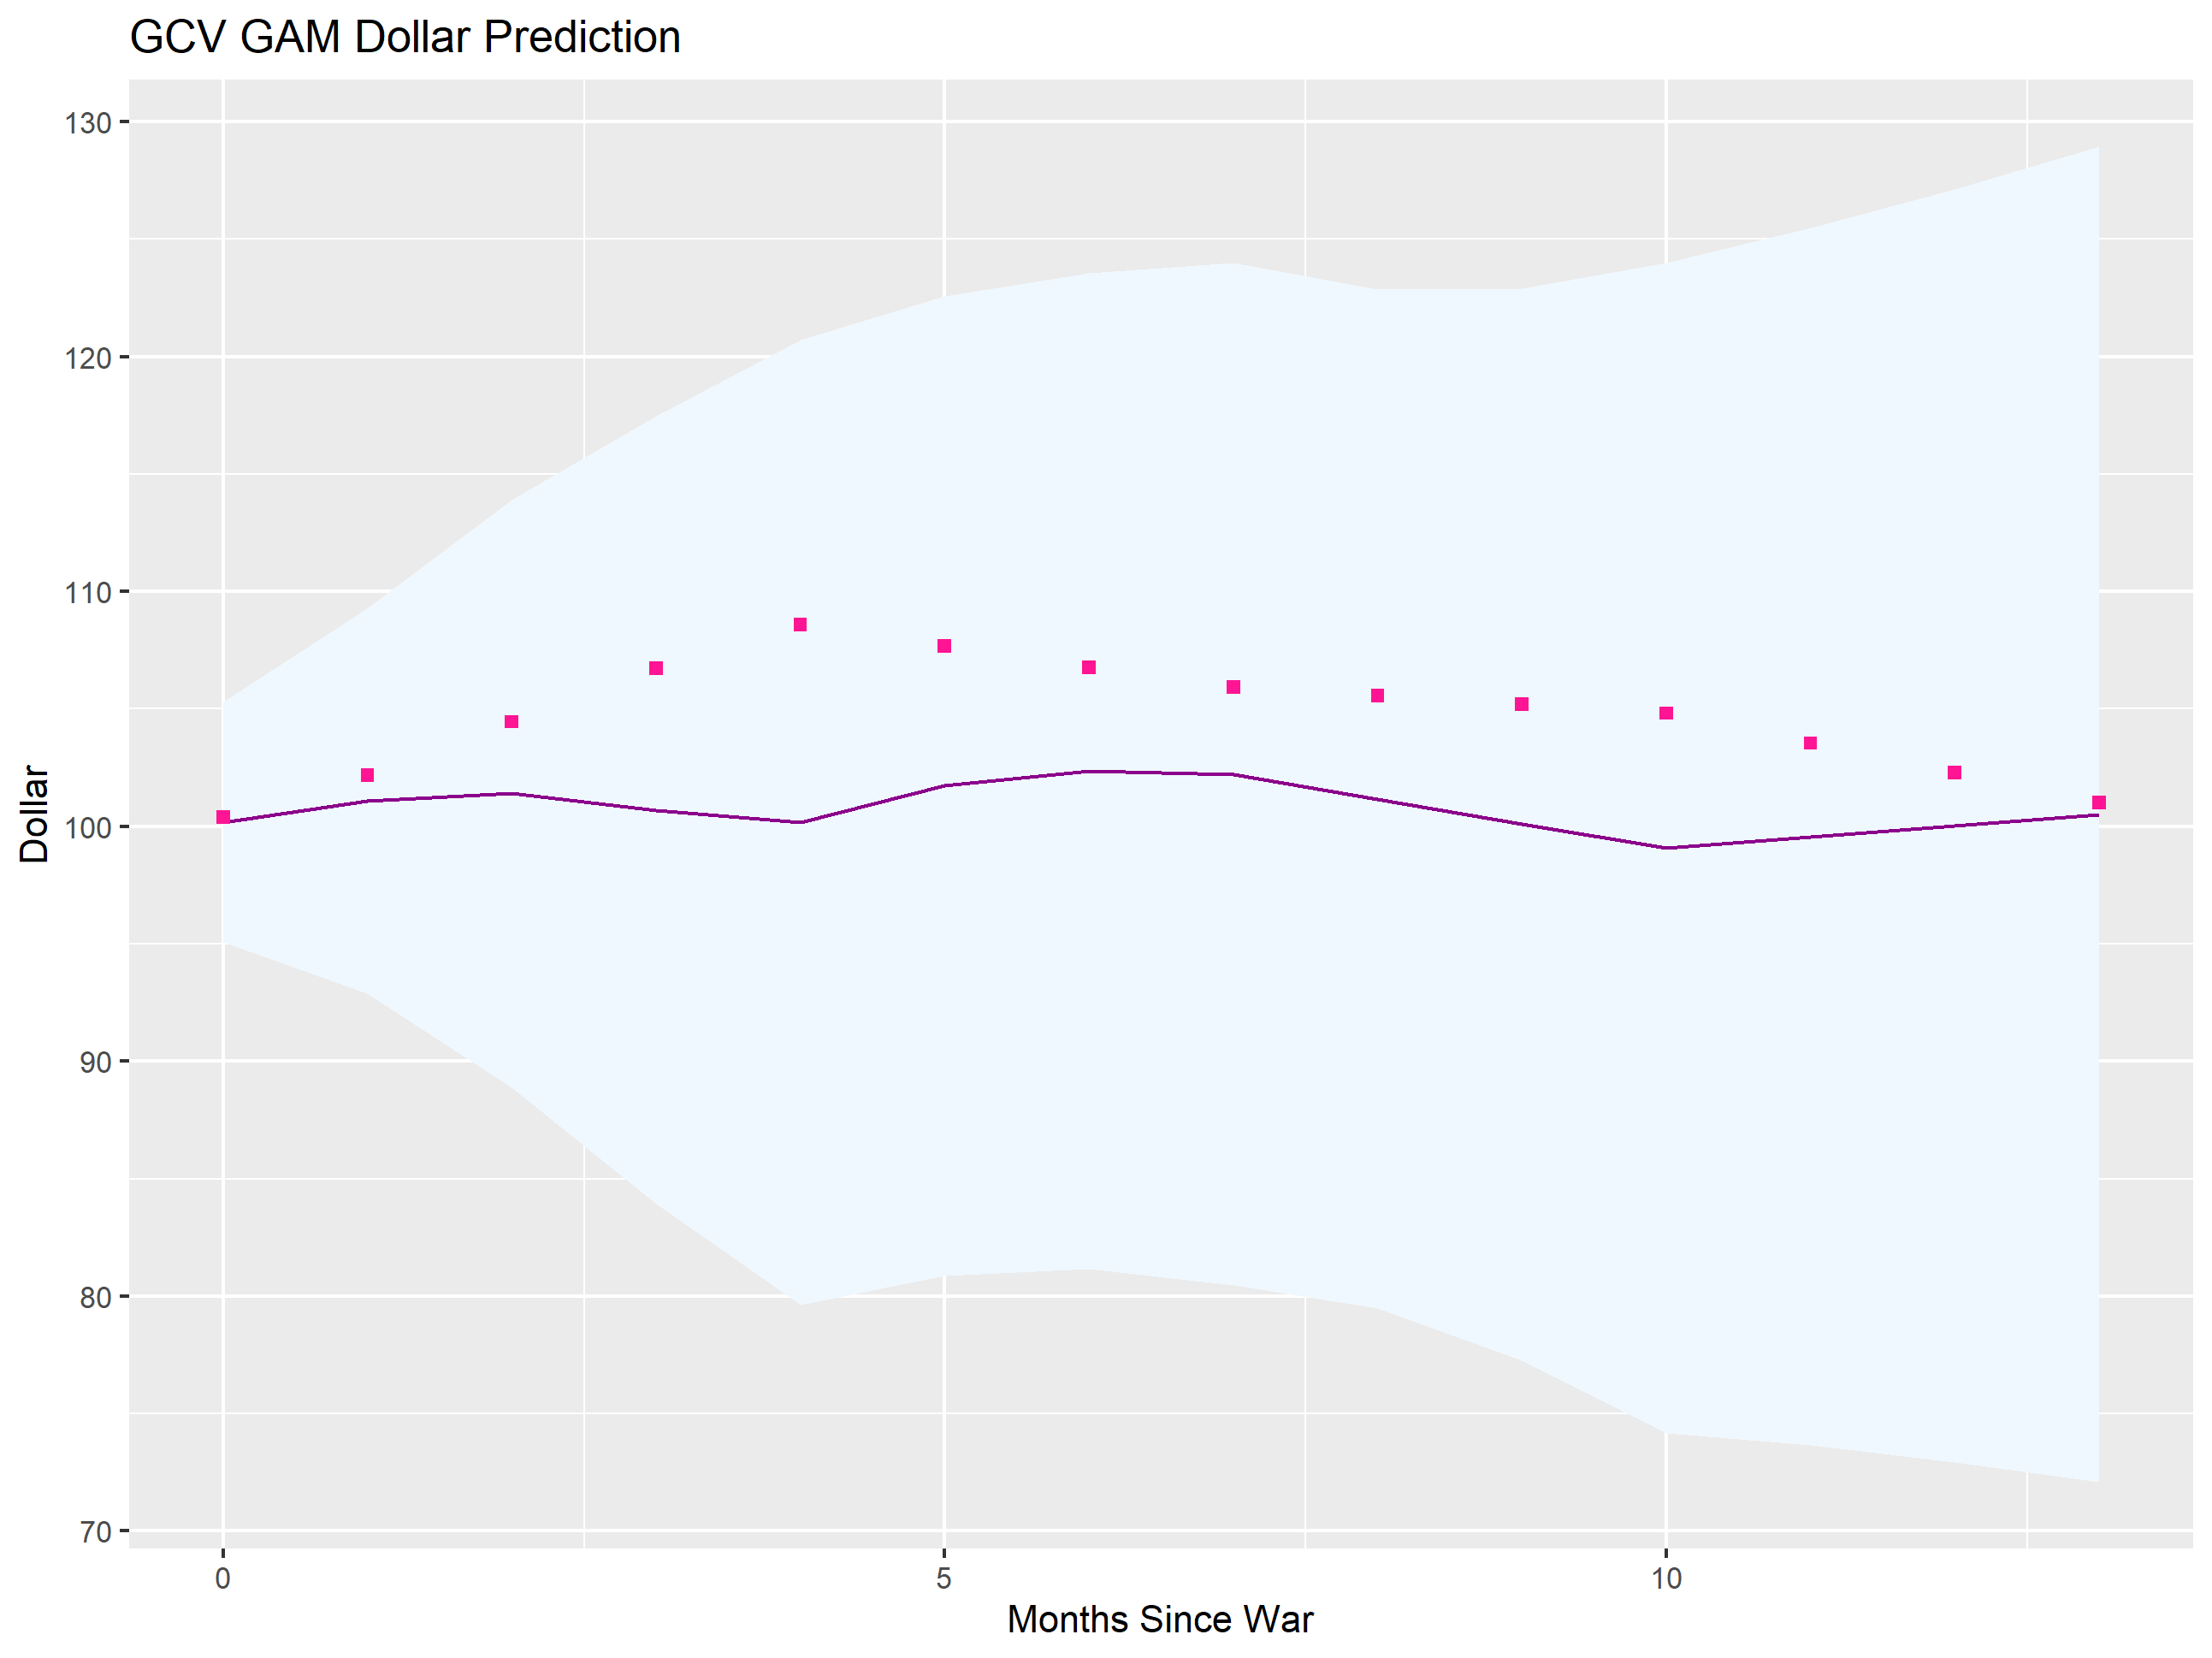
\includegraphics[width=2in]{report/us-coin-gcv.png}}
\subfigure{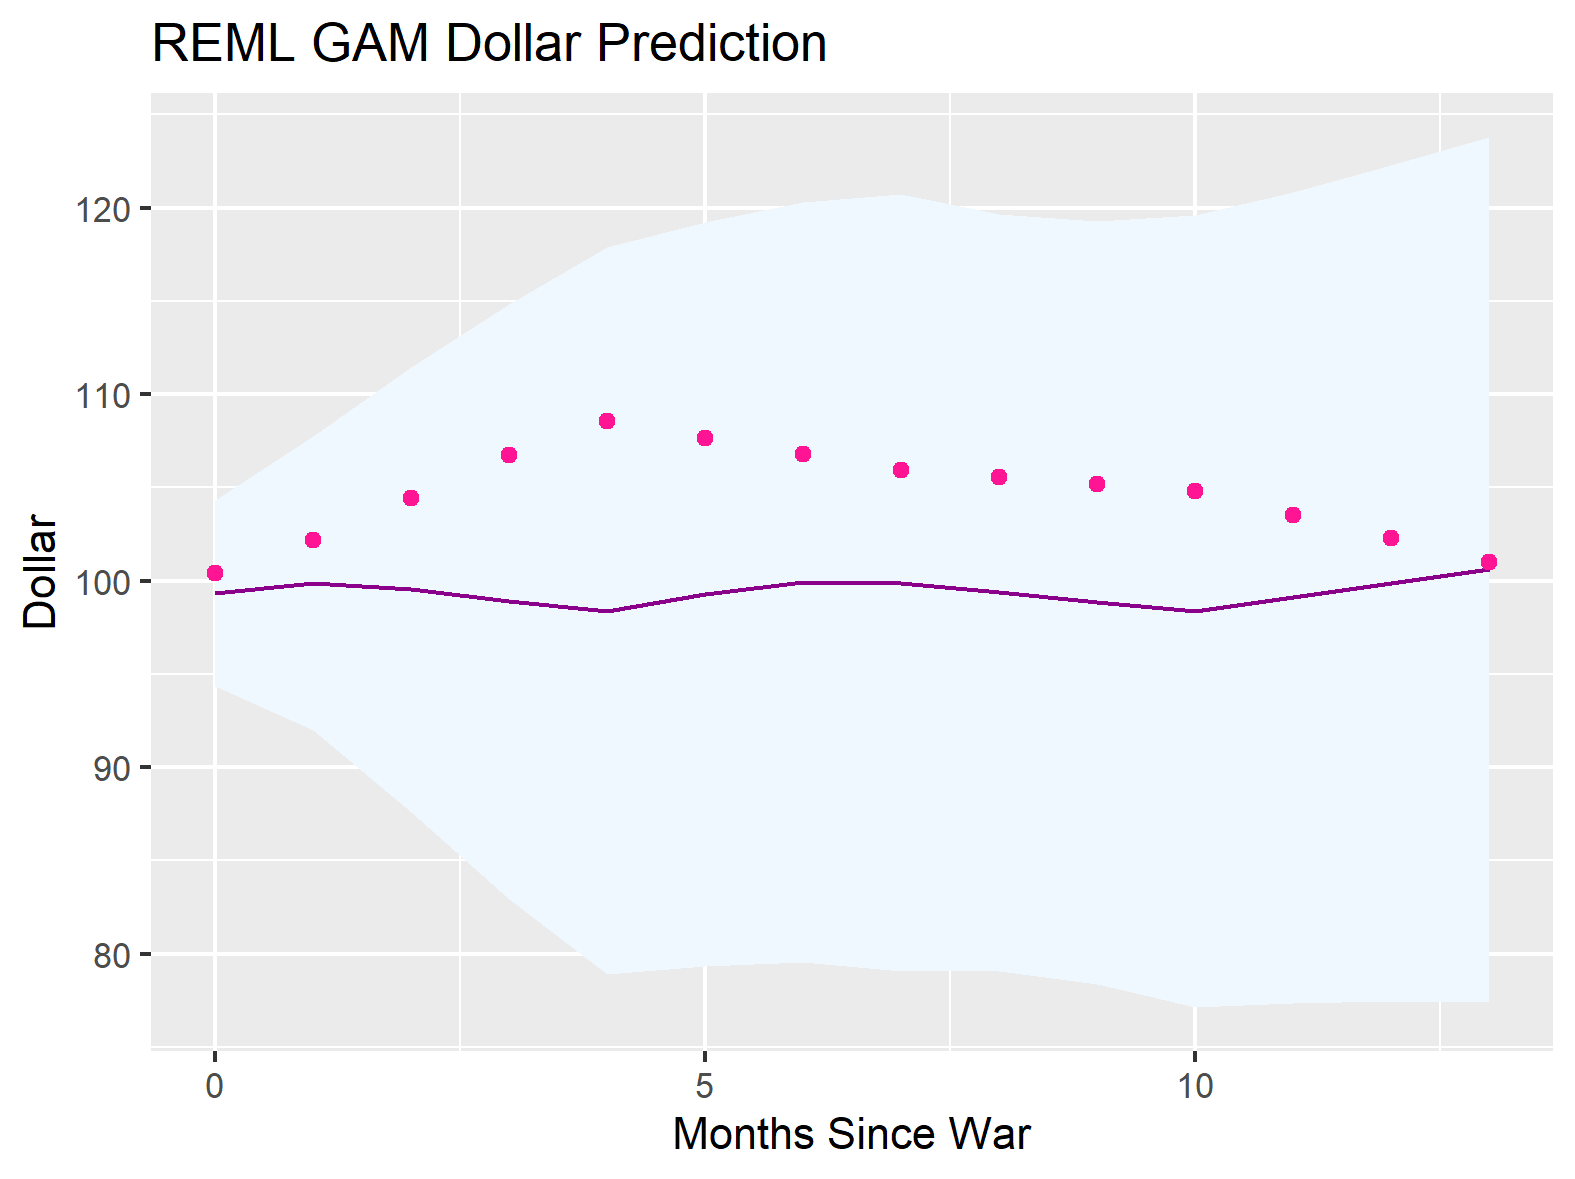
\includegraphics[width=2in]{report/us-coin-reml.png}}
}}
\caption{GAM models forecasts of GDP and the Dollar for the United States using GCV and REML methods, with true observation values represented by the pink dots.}
\end{figure}


\begin{figure}
\centering
\centerline{ \mbox{
\subfigure{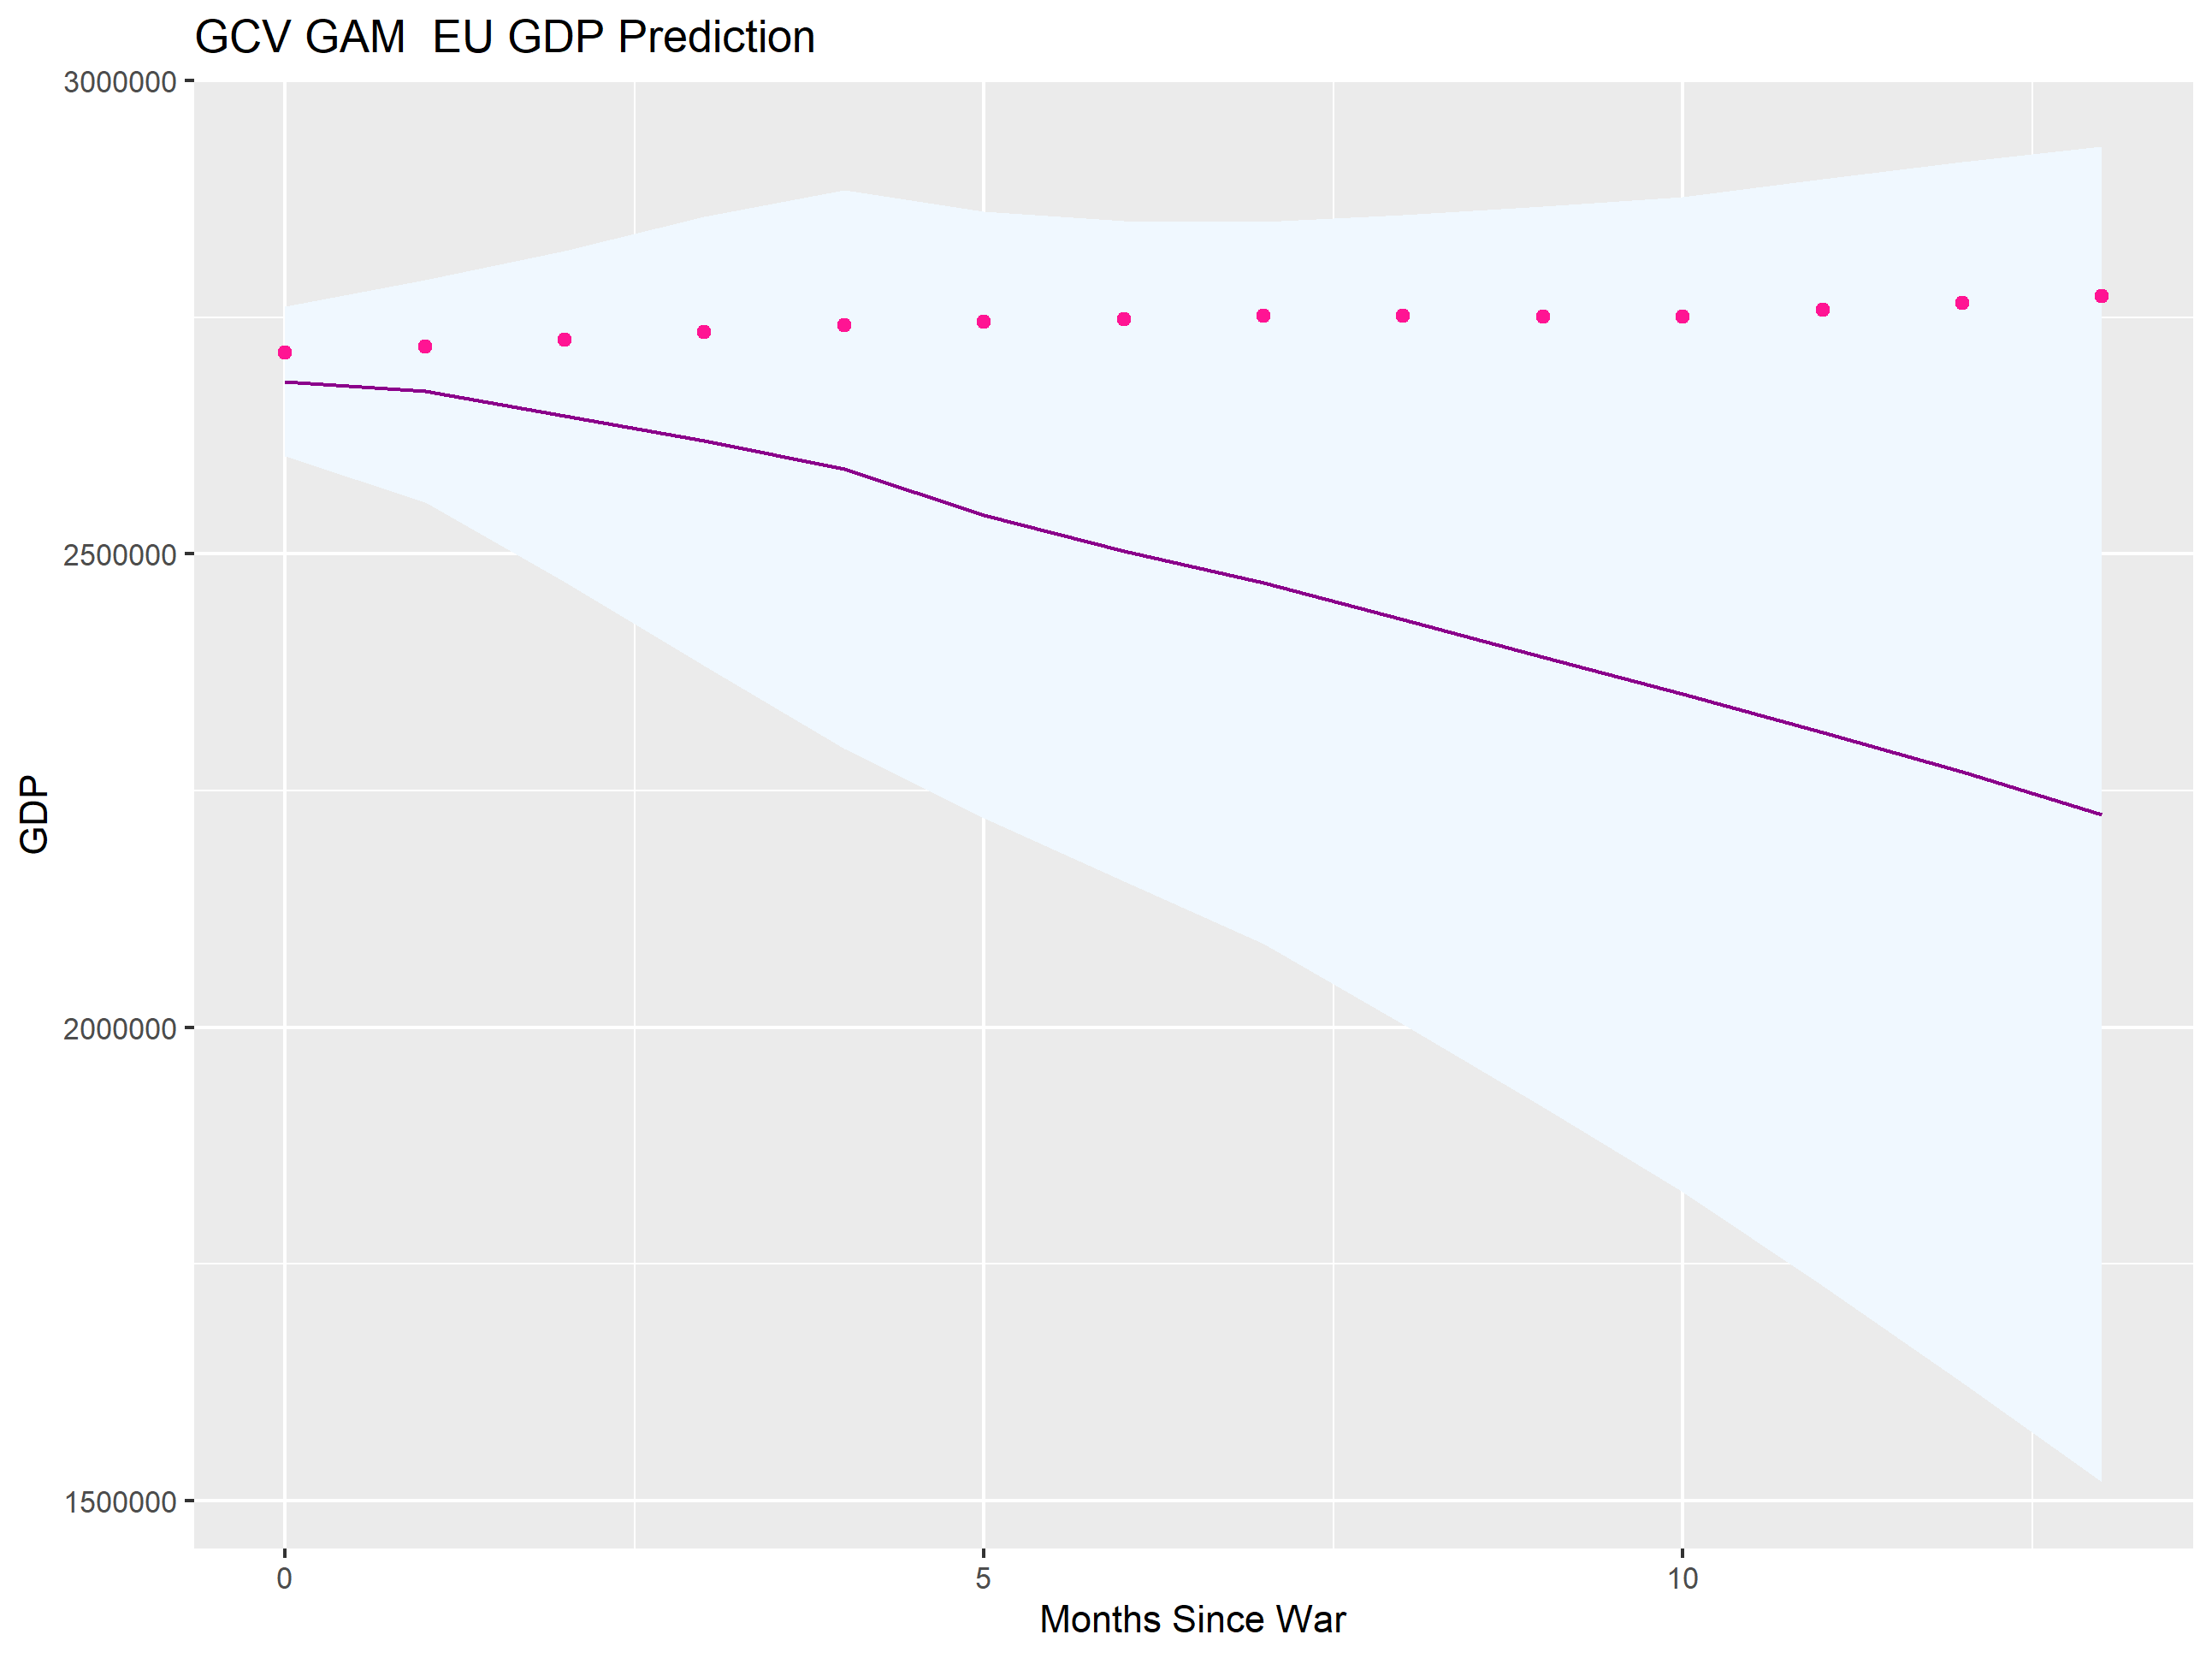
\includegraphics[width=2.2in]{report/eu-gdp-gcv.png}}  \quad
\subfigure{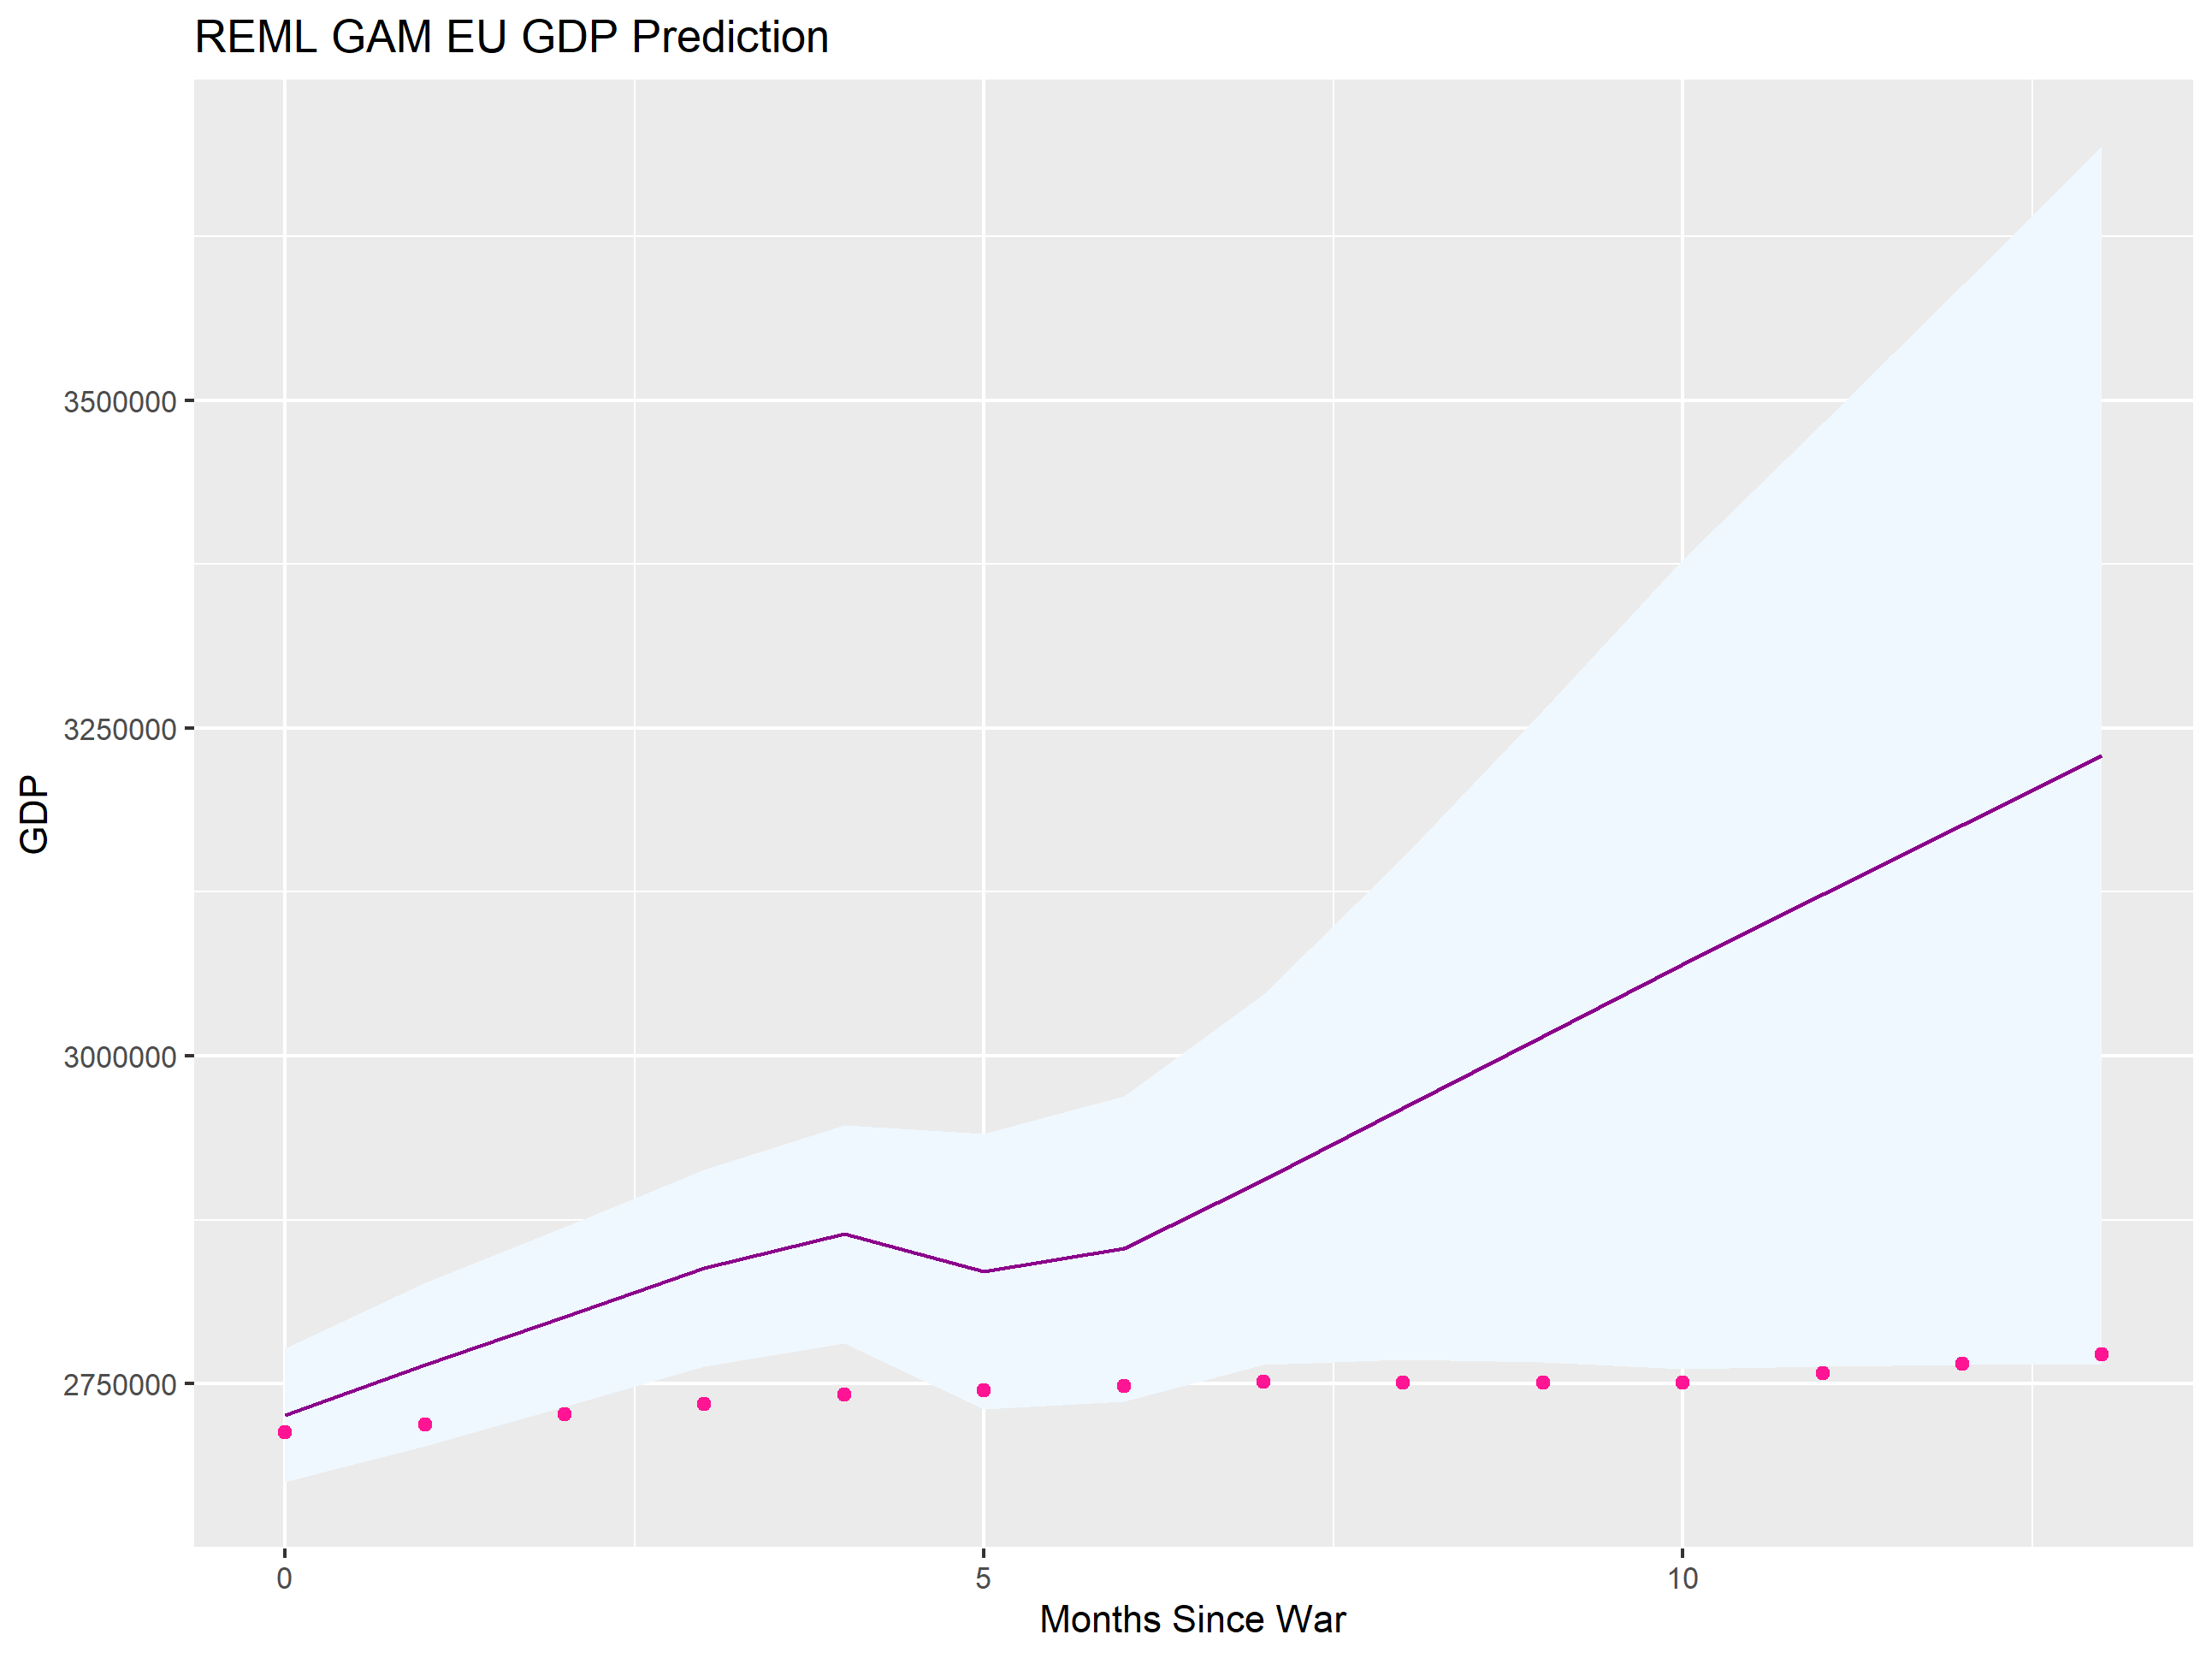
\includegraphics[width=2.2in]{eu-gdp-reml.png}}
}}
\caption{GAM models forecasts of GDP for the European union using GCV and REML methods, with true observation values represented by the pink dots.  }
\end{figure}

\begin{figure}
\centering
\centerline{ \mbox{
\subfigure{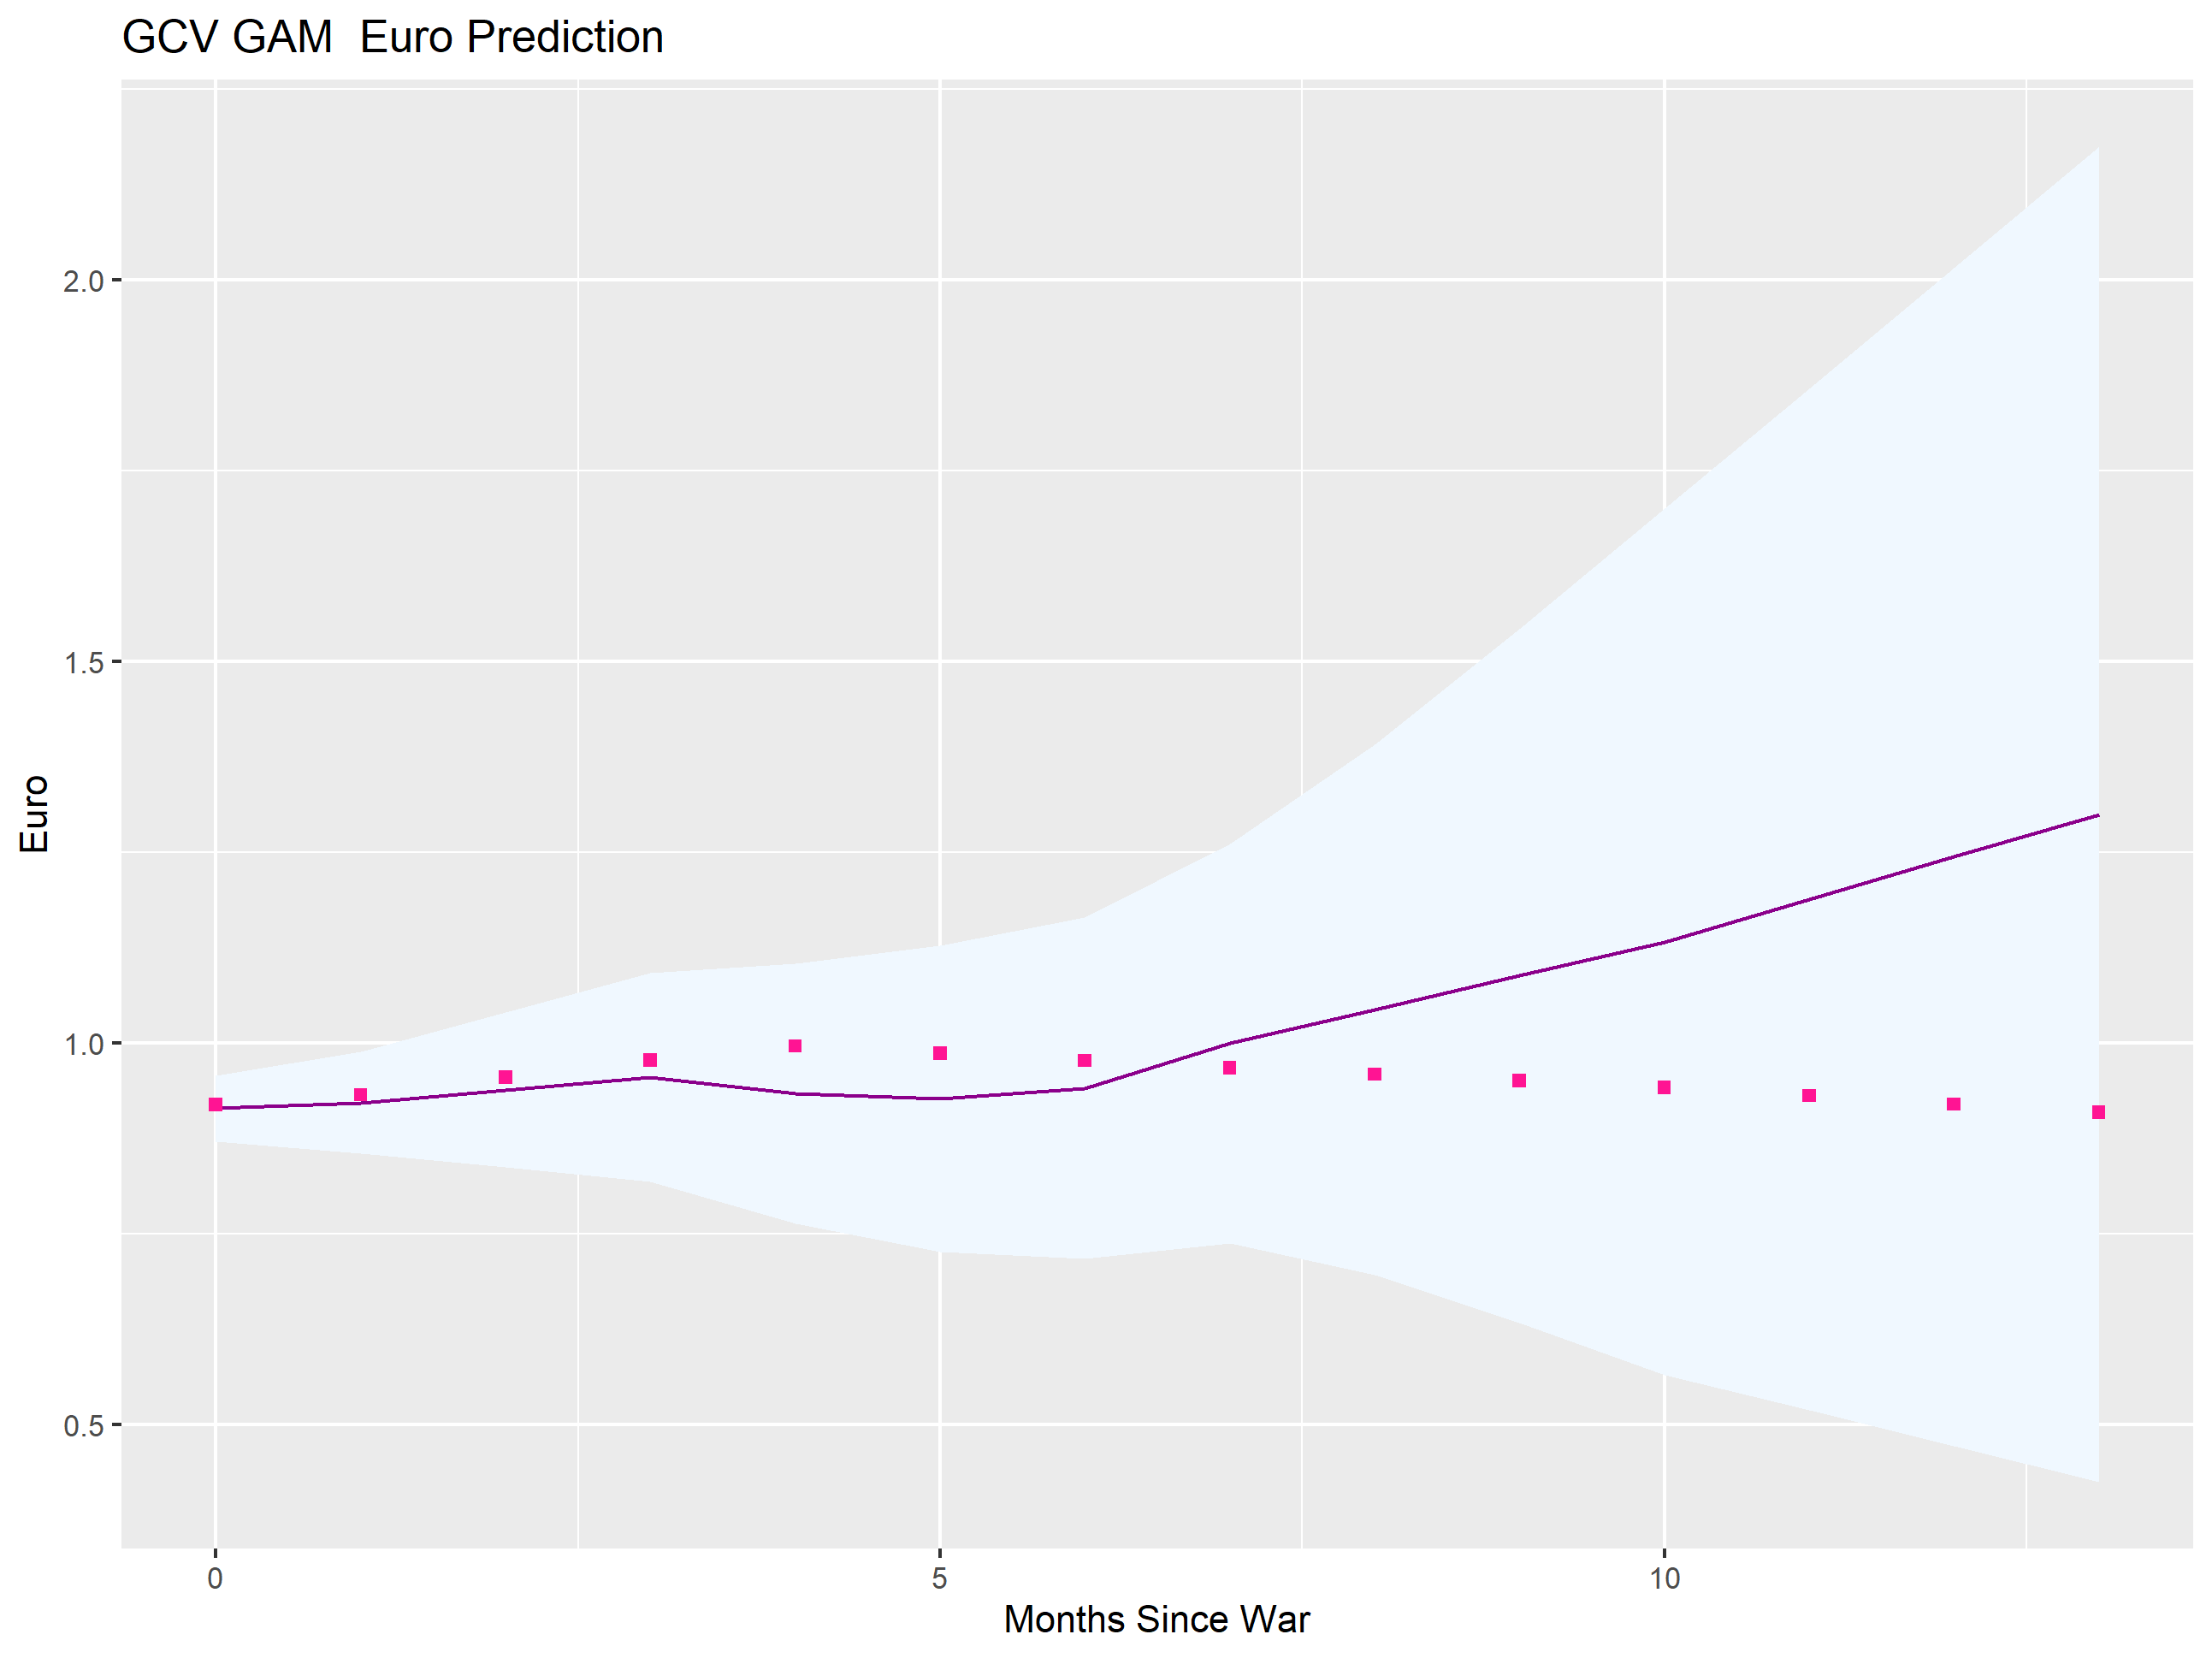
\includegraphics[width=2.2in]{report/eu-coin-gcv.png}}  \quad
\subfigure{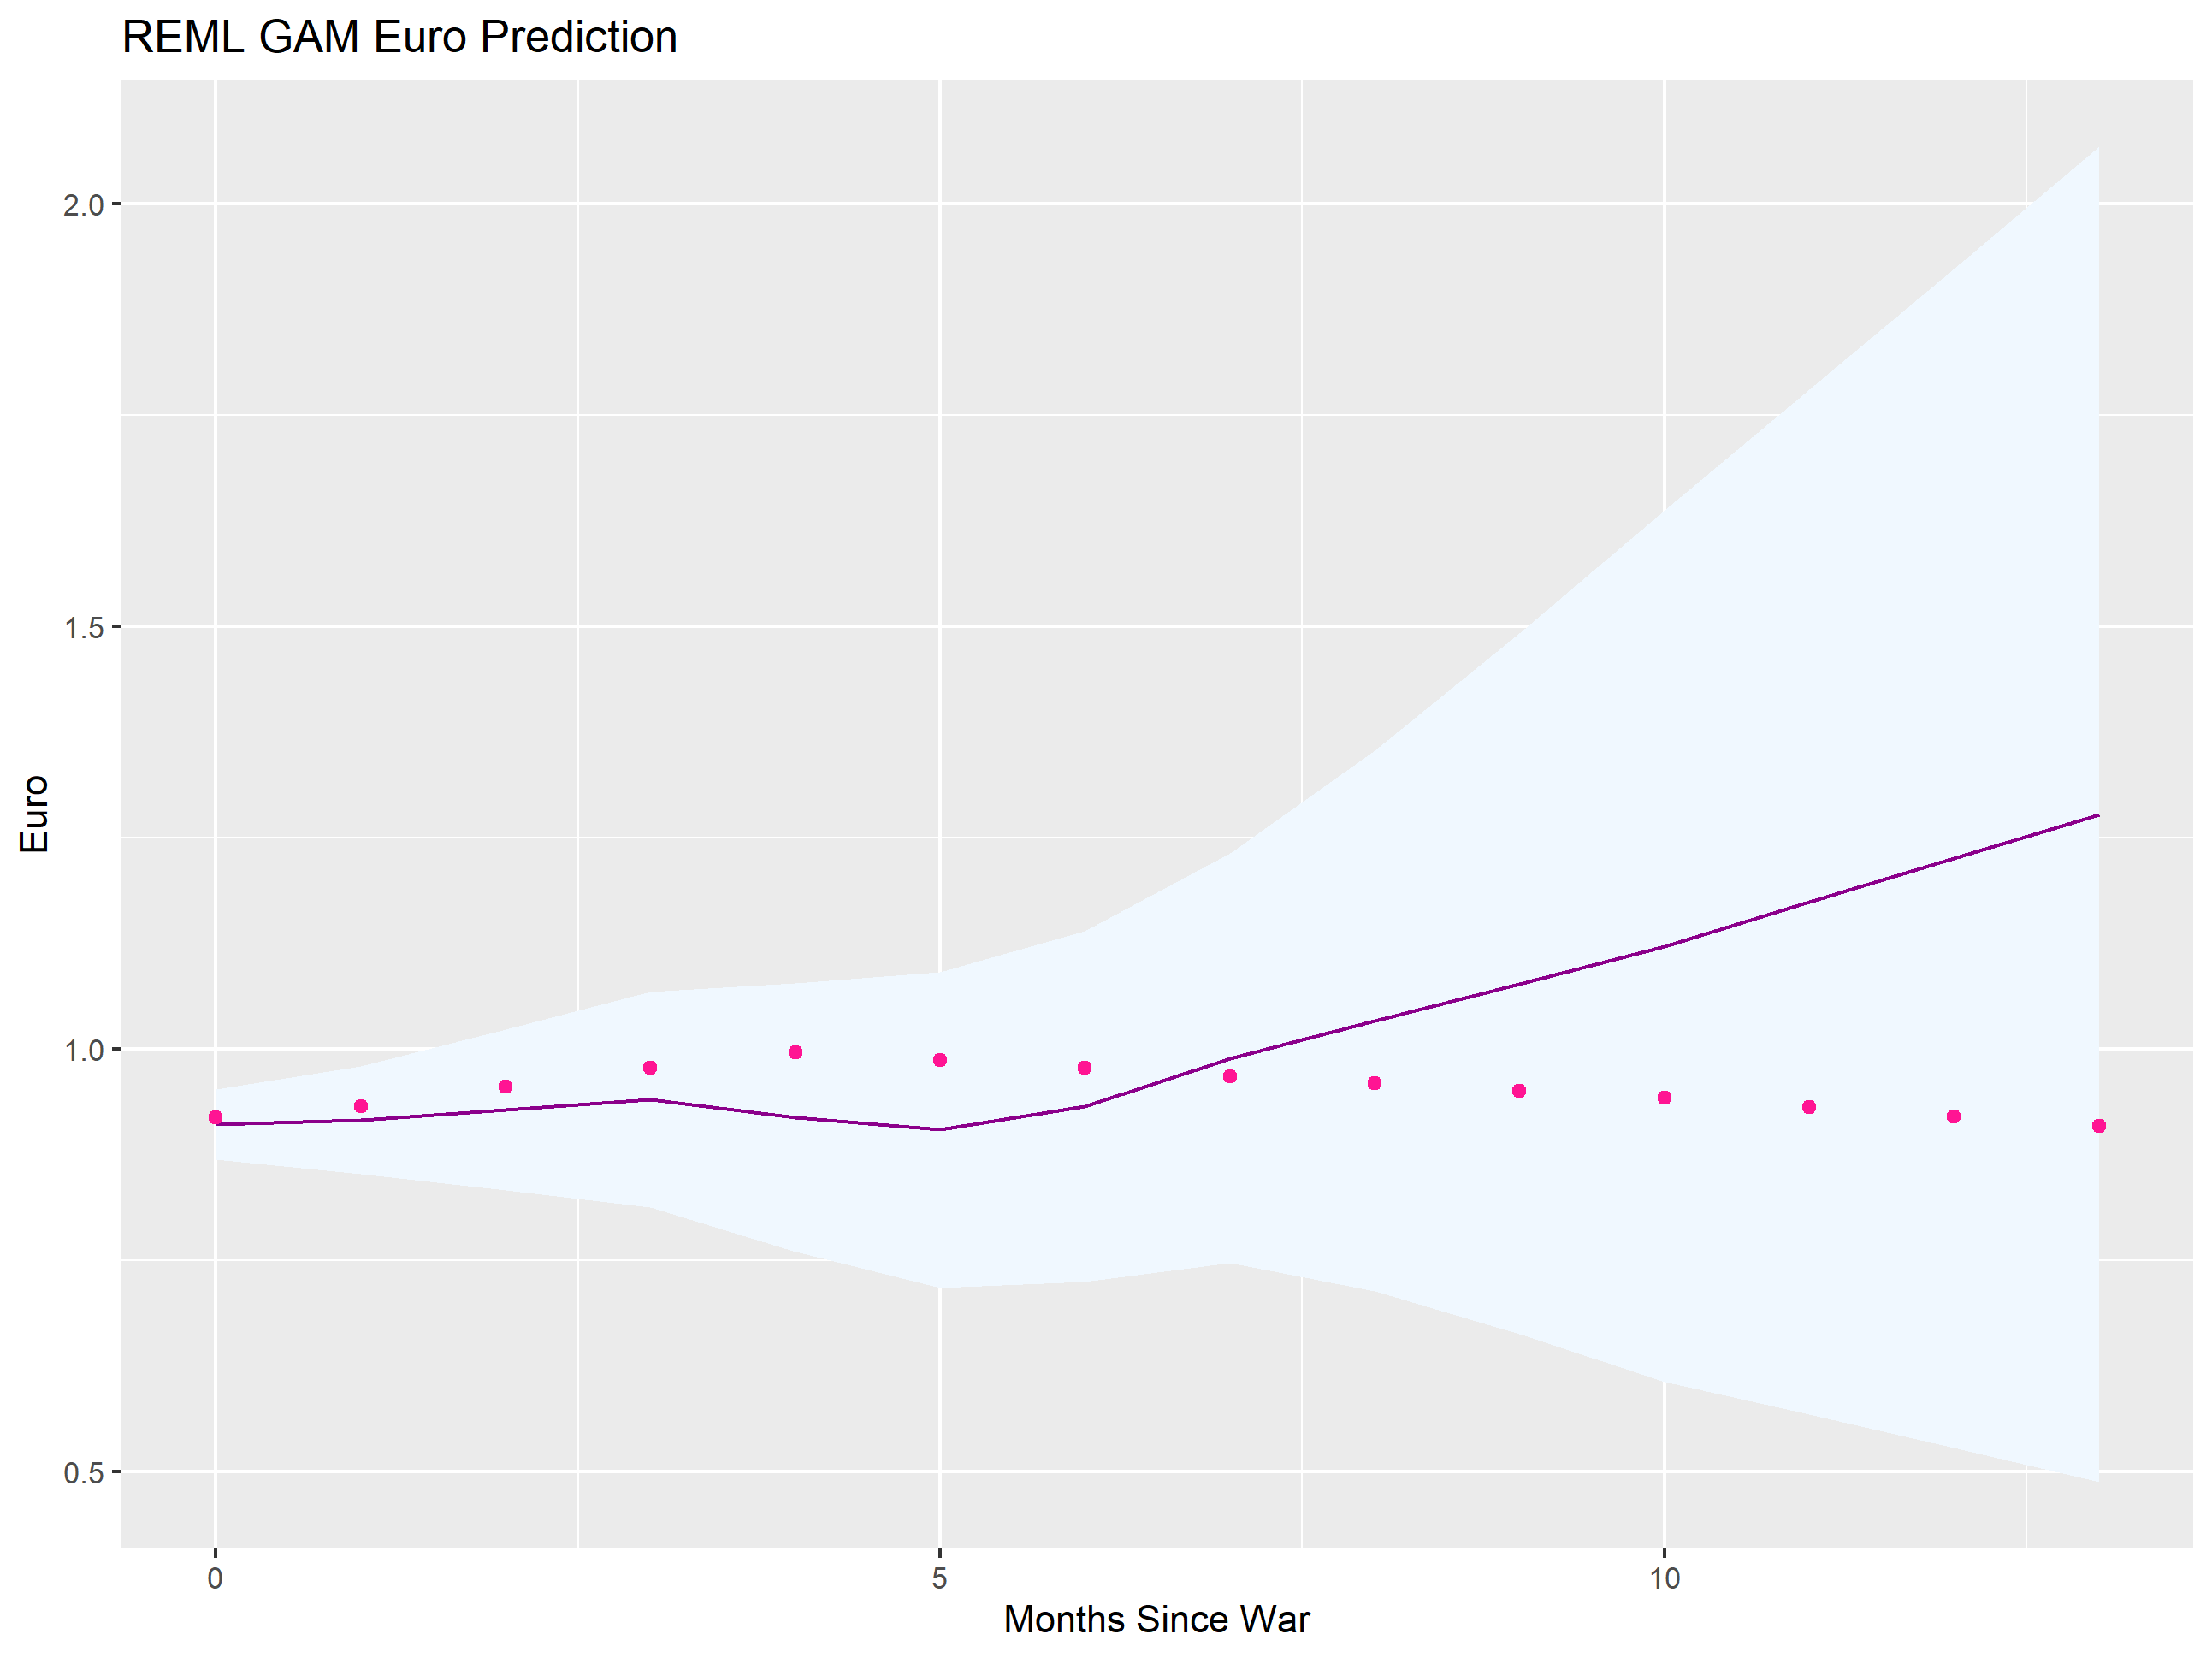
\includegraphics[width=2.2in]{report/eu-coin-reml.png}}
}}
\caption{GAM models forecasts of the Euro for the European Union using GCV and REML methods, with true observation values represented by the pink dots.  }
\end{figure}

\begin{figure}
\centering
\centerline{ \mbox{
\subfigure{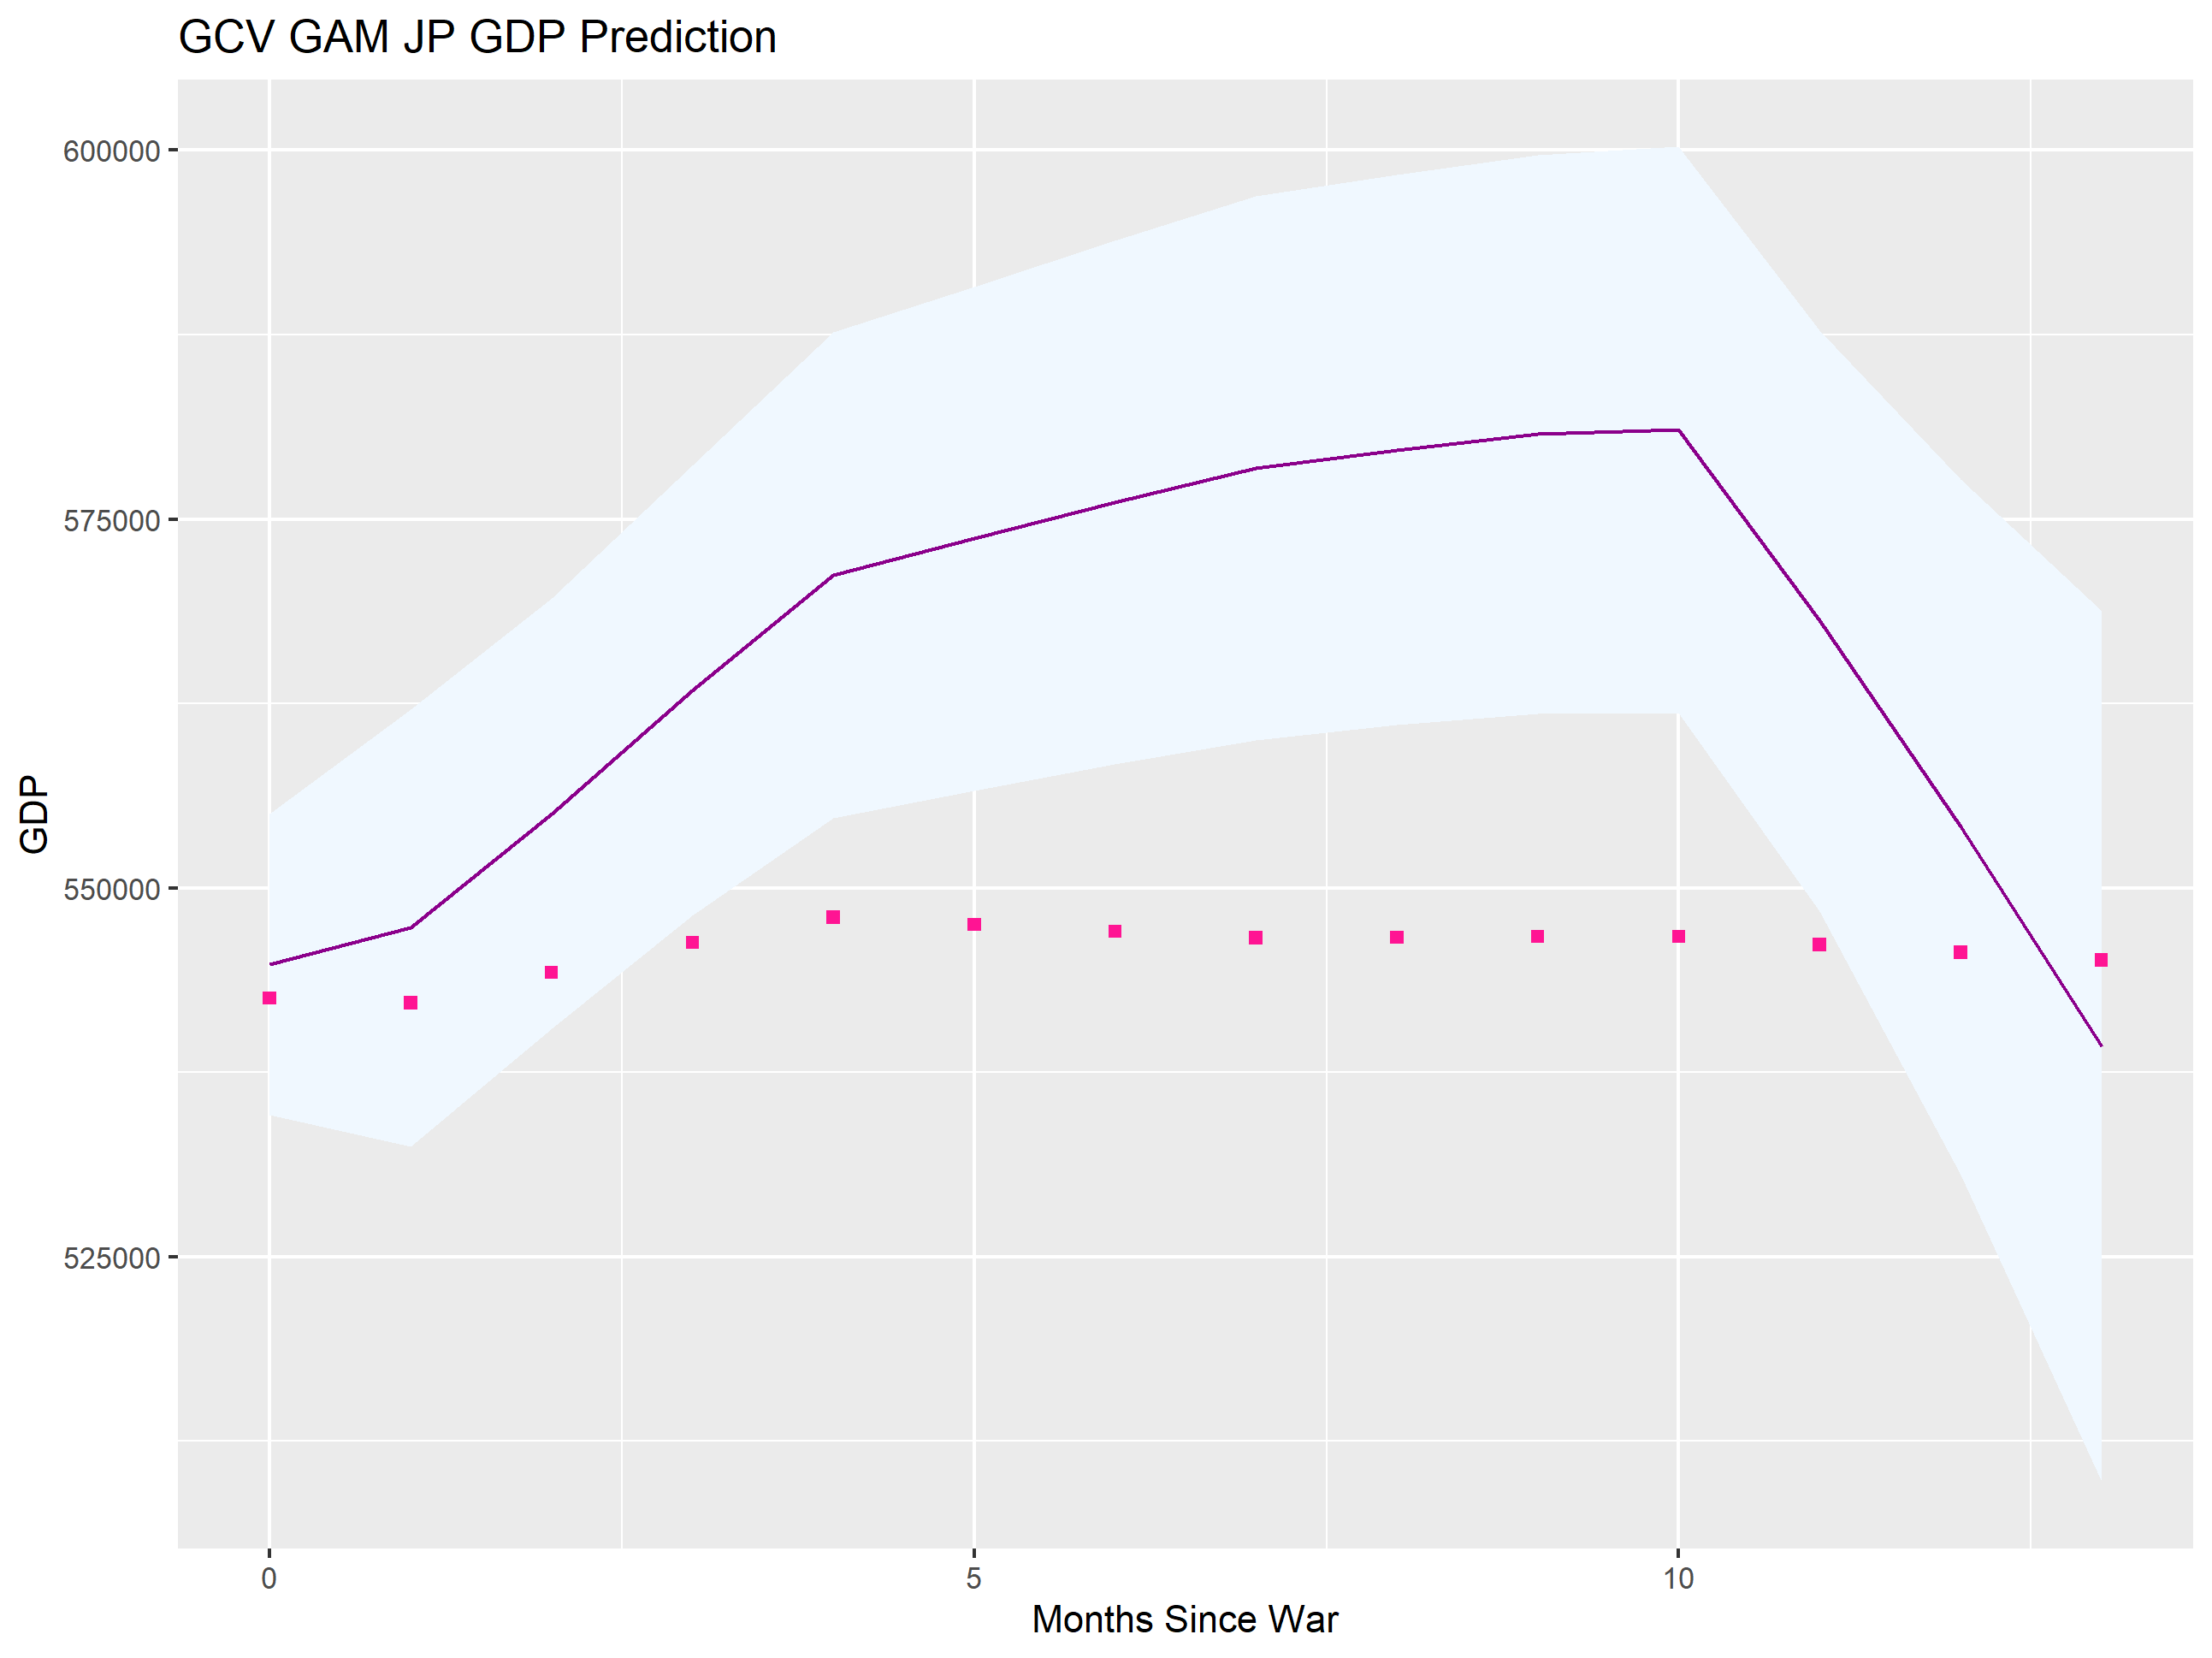
\includegraphics[width=2.2in]{report/jap-gdp-gcv.png}}  \quad
\subfigure{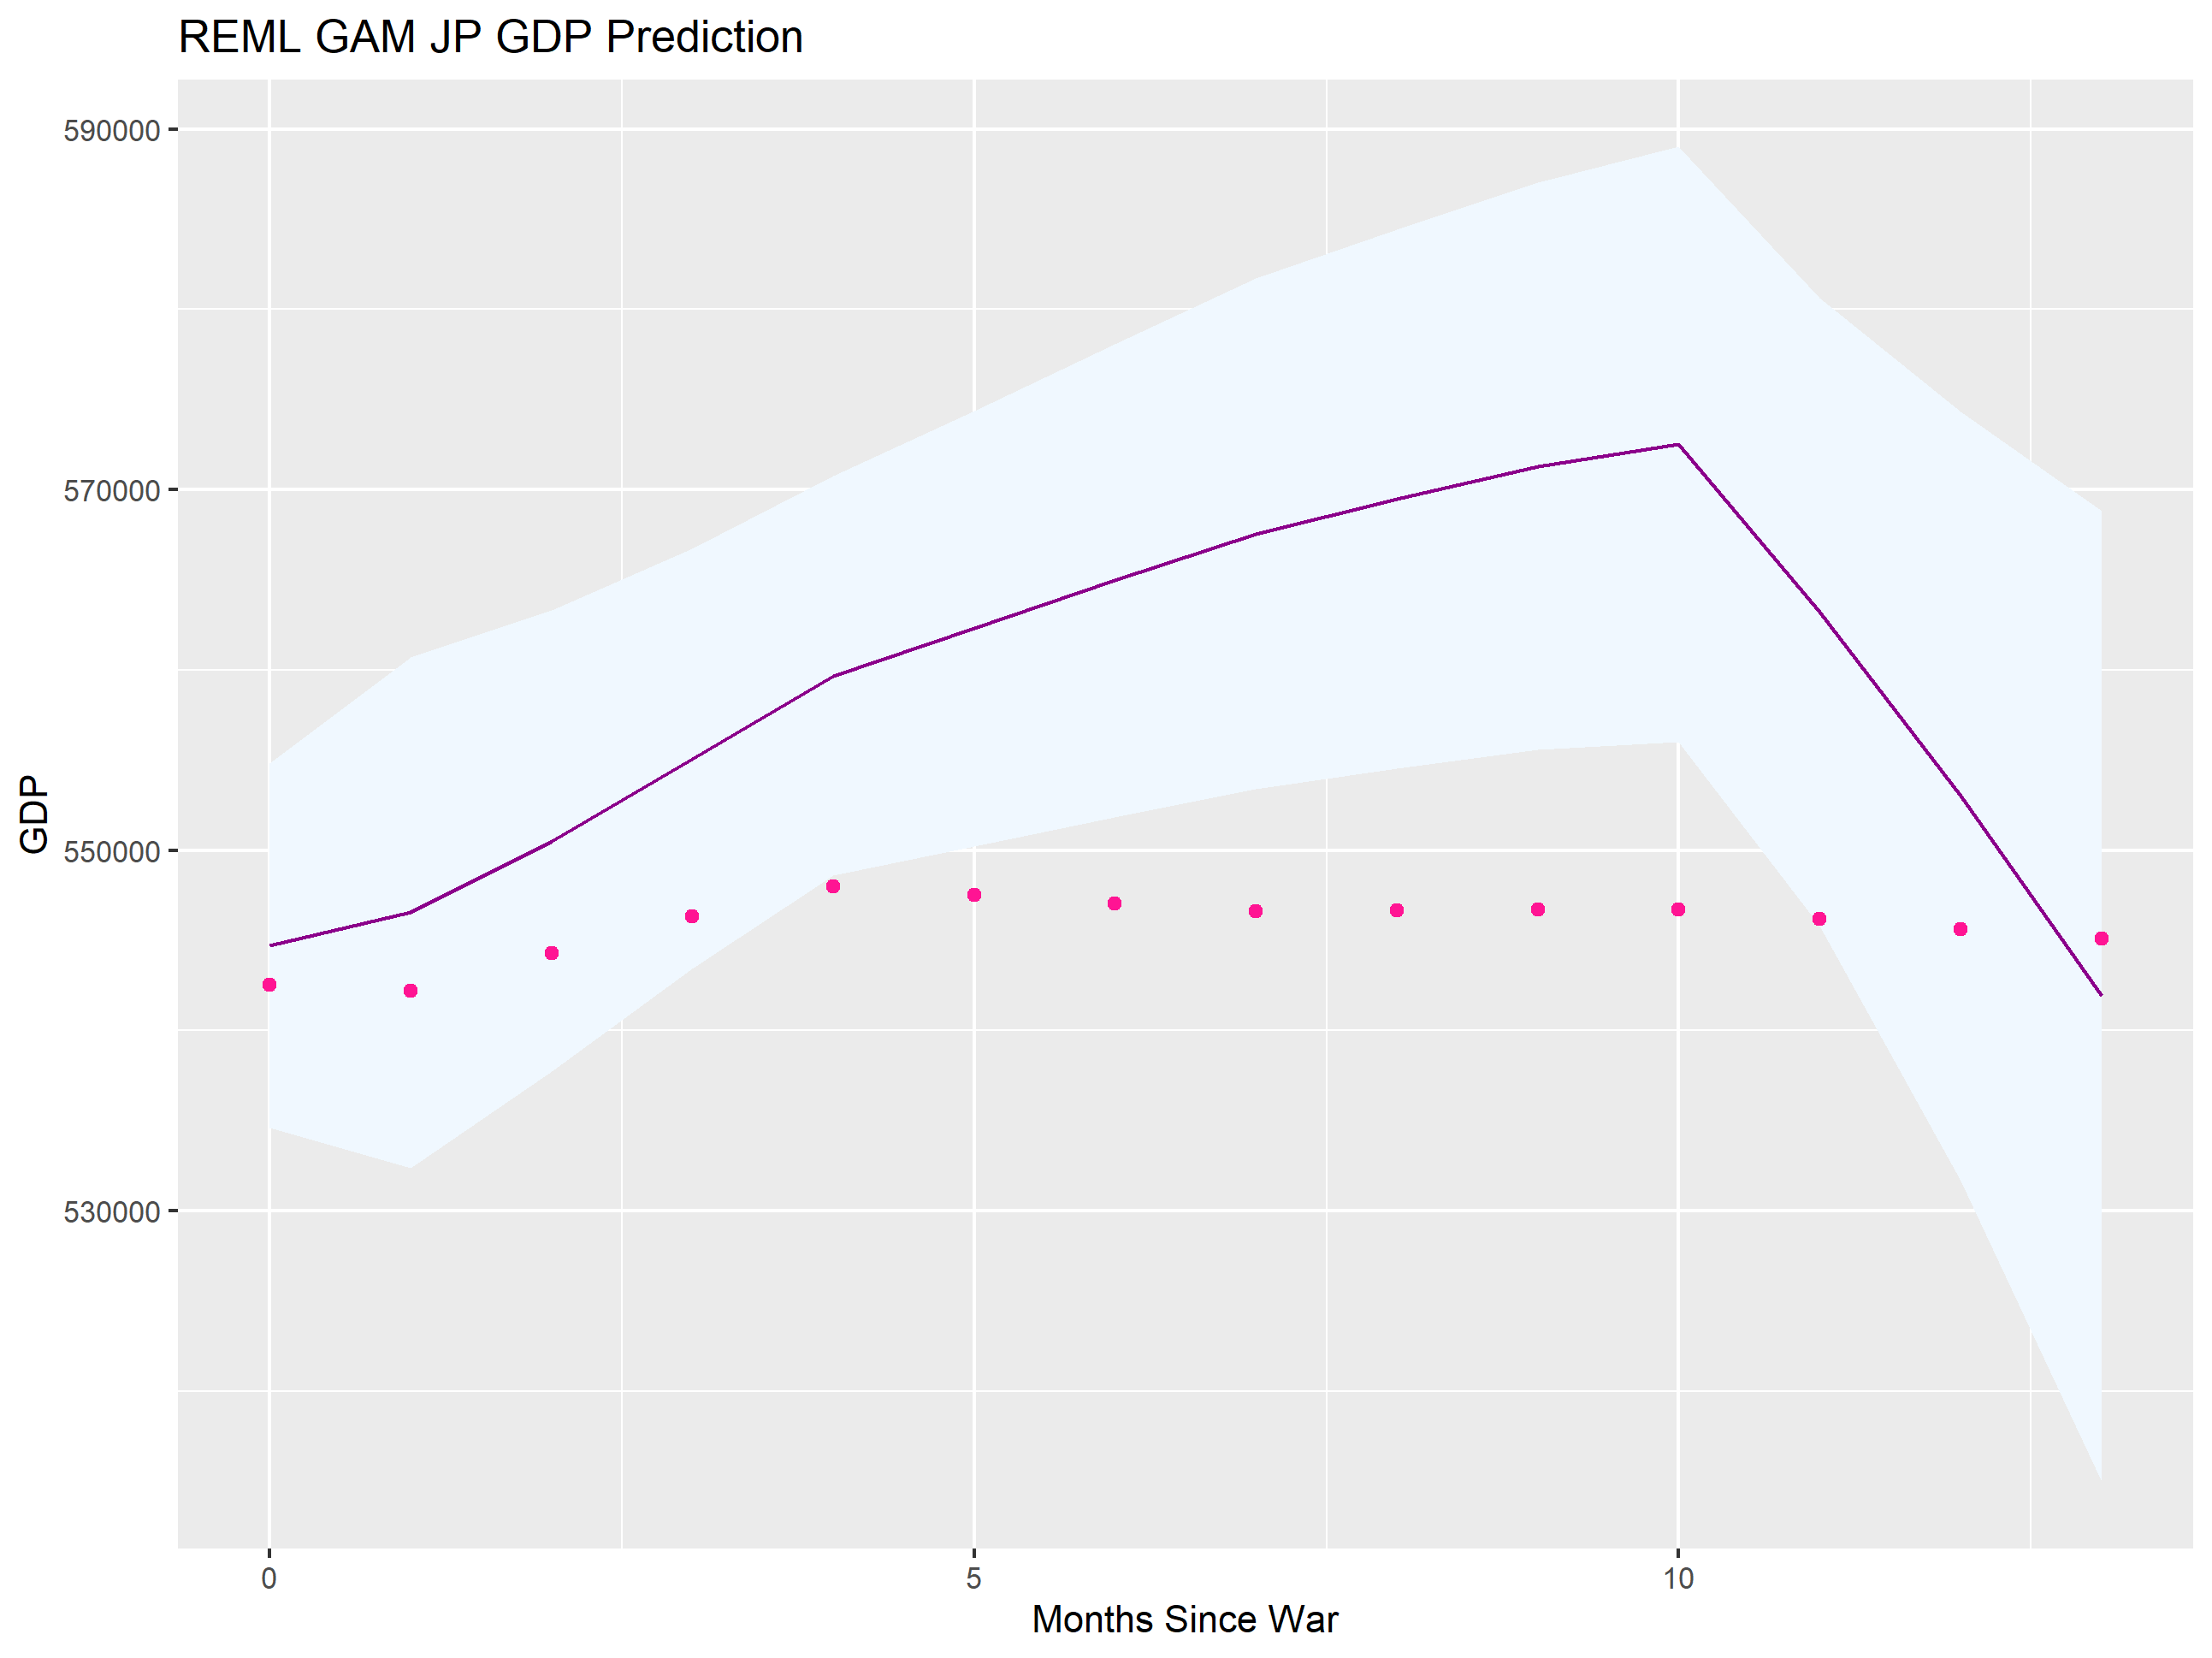
\includegraphics[width=2.2in]{jap-gdp-reml.png}}
}}
\caption{GAM models forecasts of GDP for Japan using GCV and REML methods, with true observation values represented by the pink dots.}
\end{figure}

\begin{figure}
\centering
\centerline{ \mbox{
\subfigure{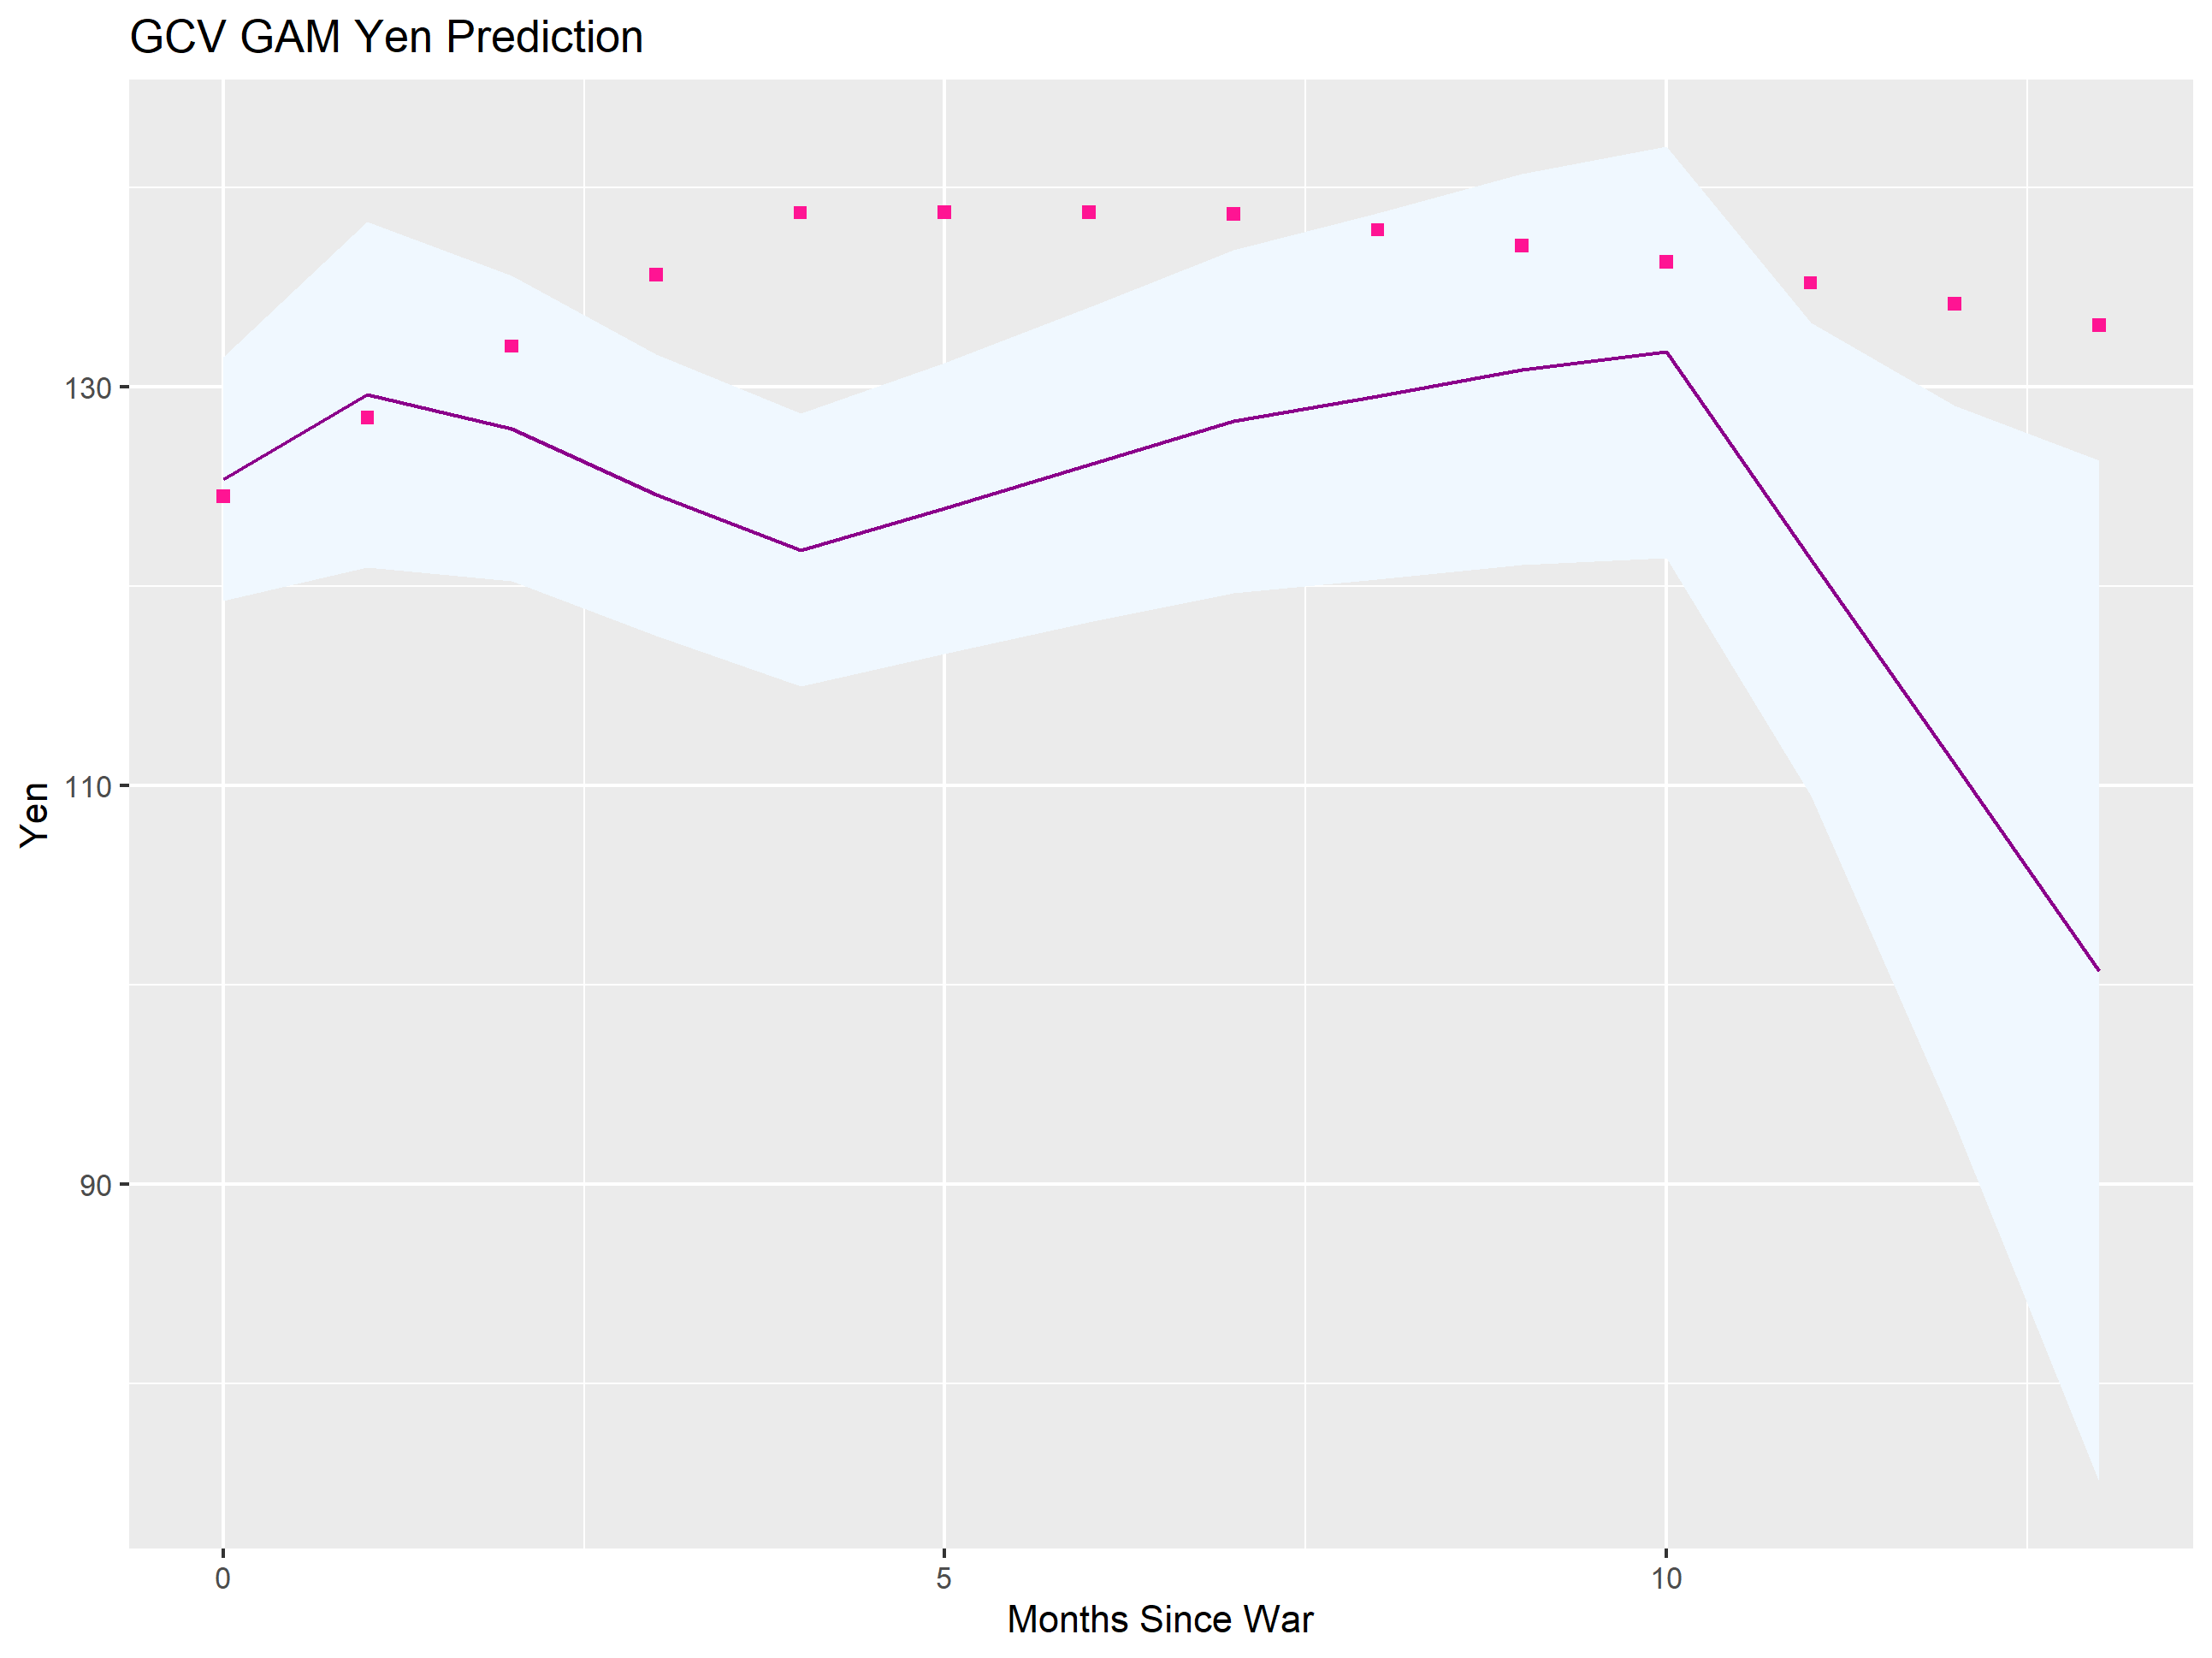
\includegraphics[width=2.2in]{report/jap-coin-gcv.png}}  \quad
\subfigure{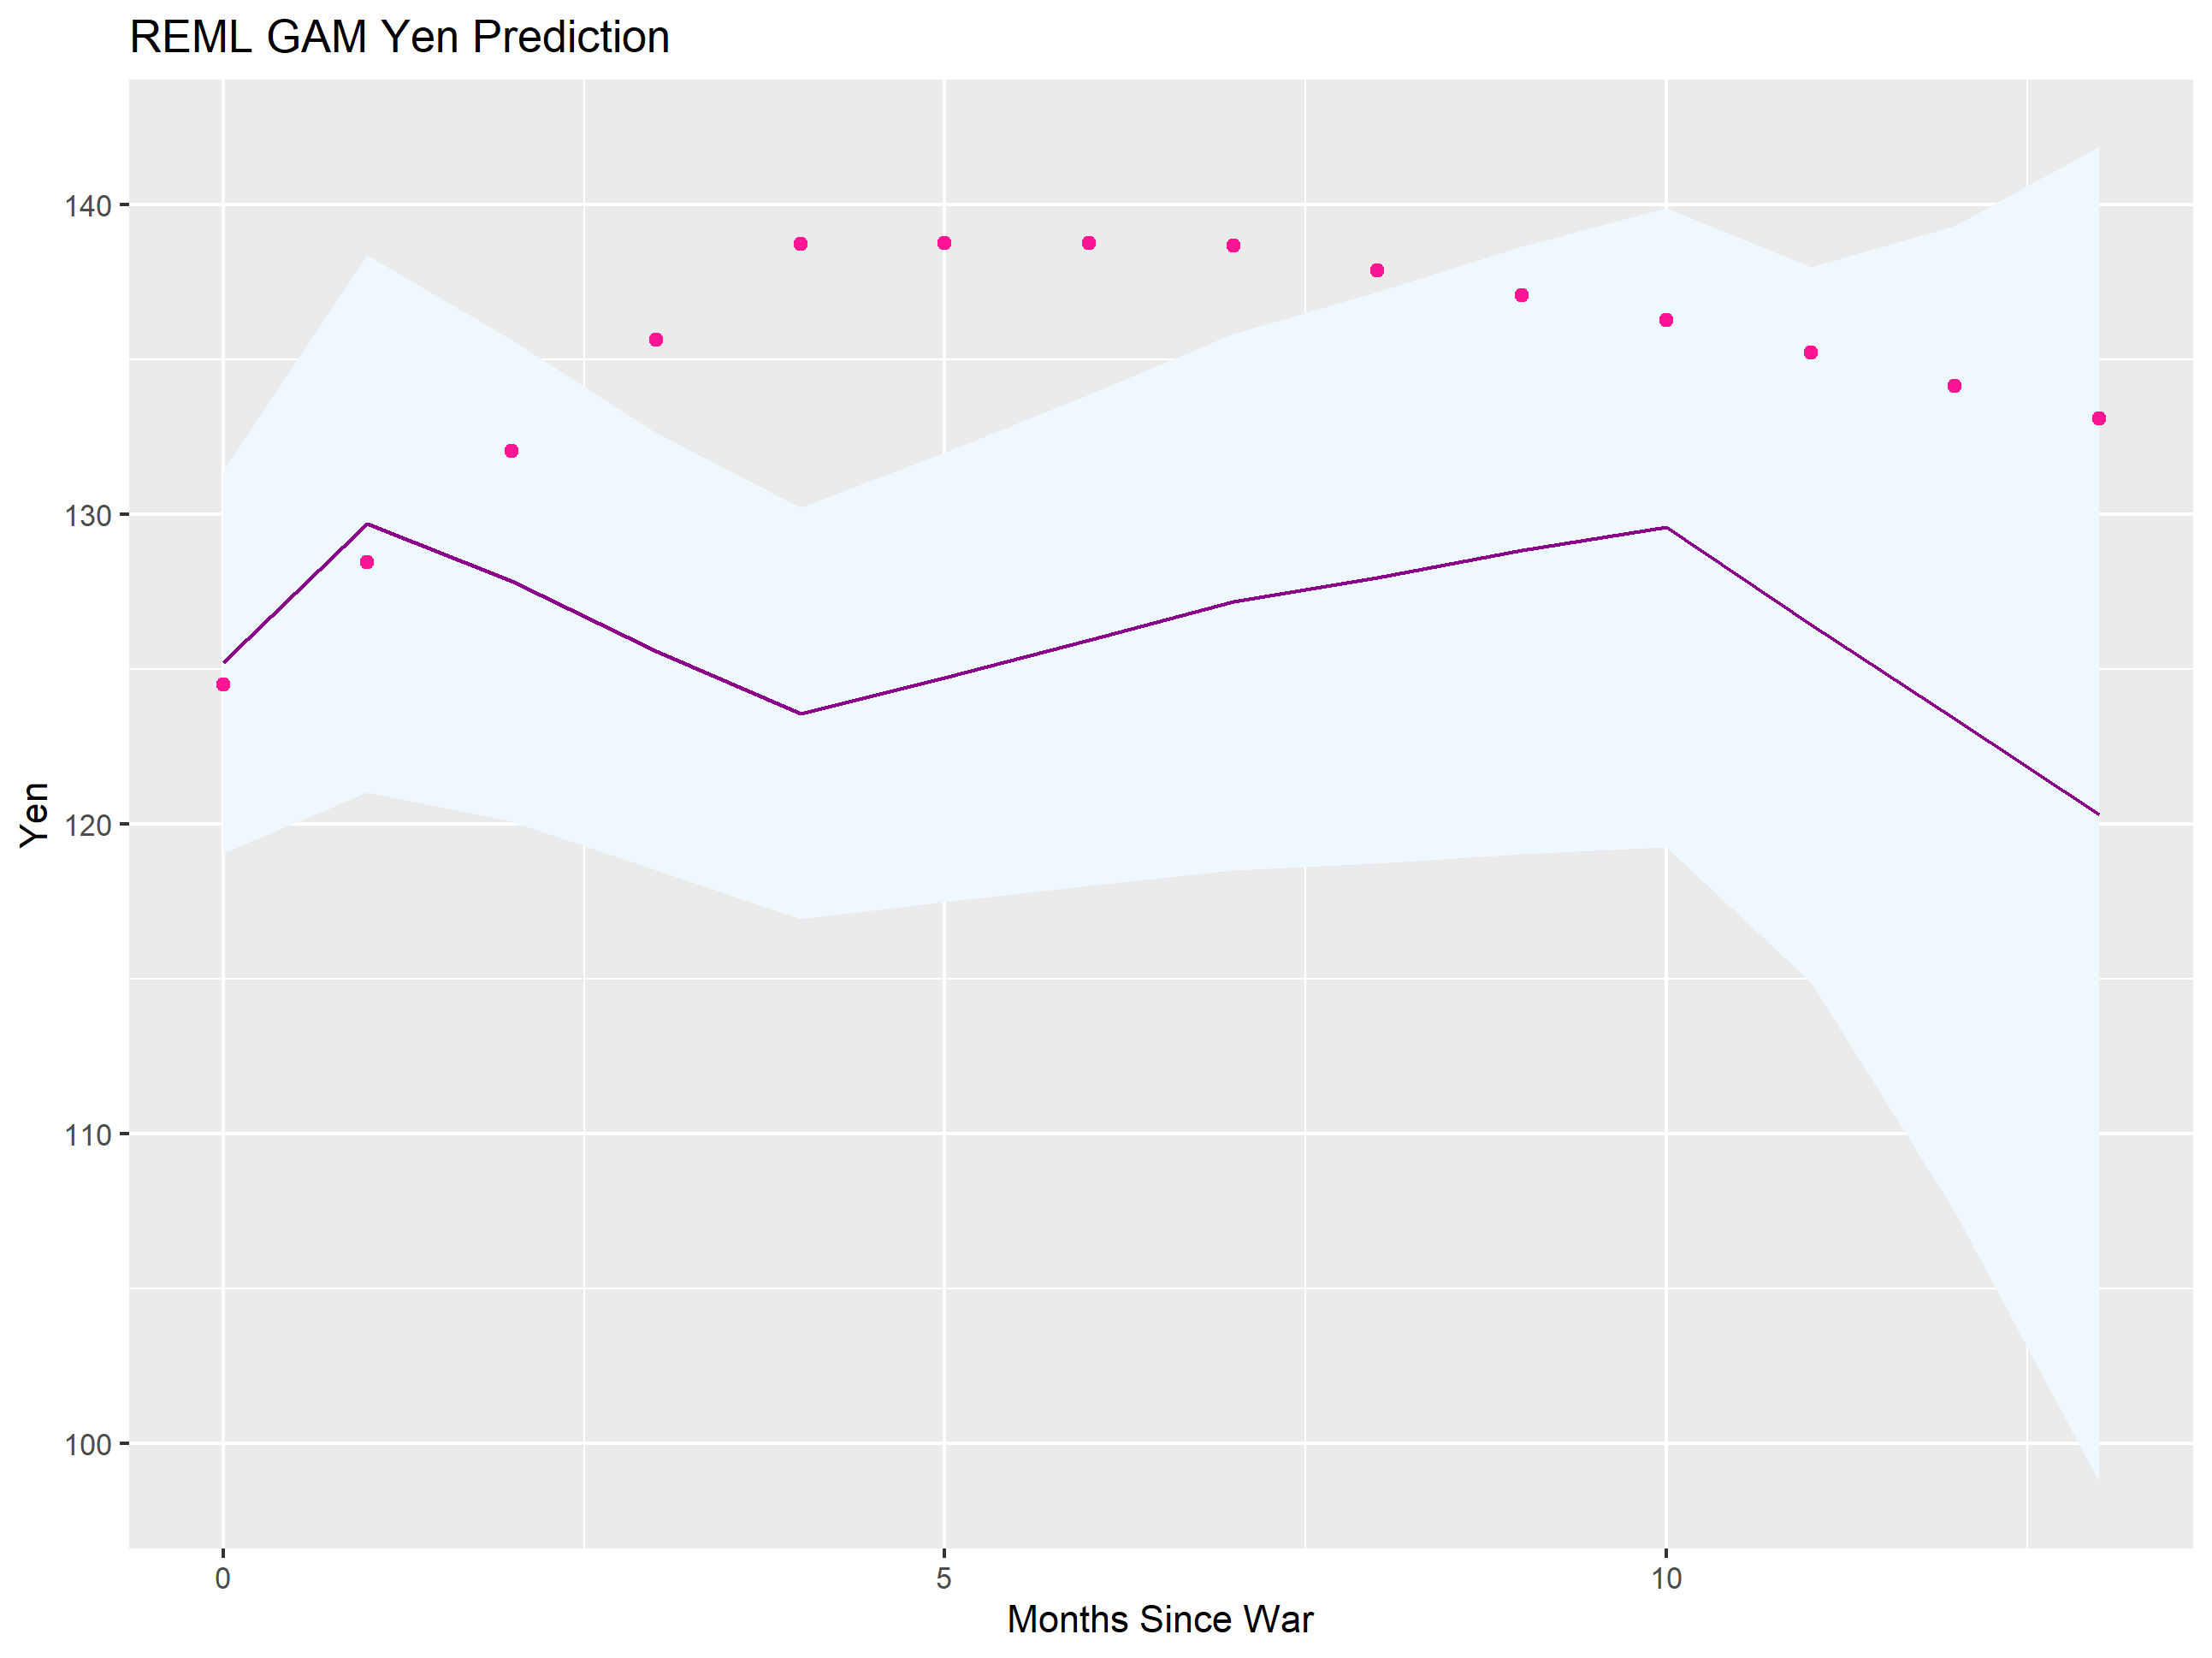
\includegraphics[width=2.2in]{report/jap-coin-reml.png}}
}}
\caption{GAM models forecasts of the Yen for Japan using GCV and REML methods, with true observation values represented by the pink dots. }
\end{figure}


\begin{figure}
\centering
\centerline{ \mbox{
\subfigure{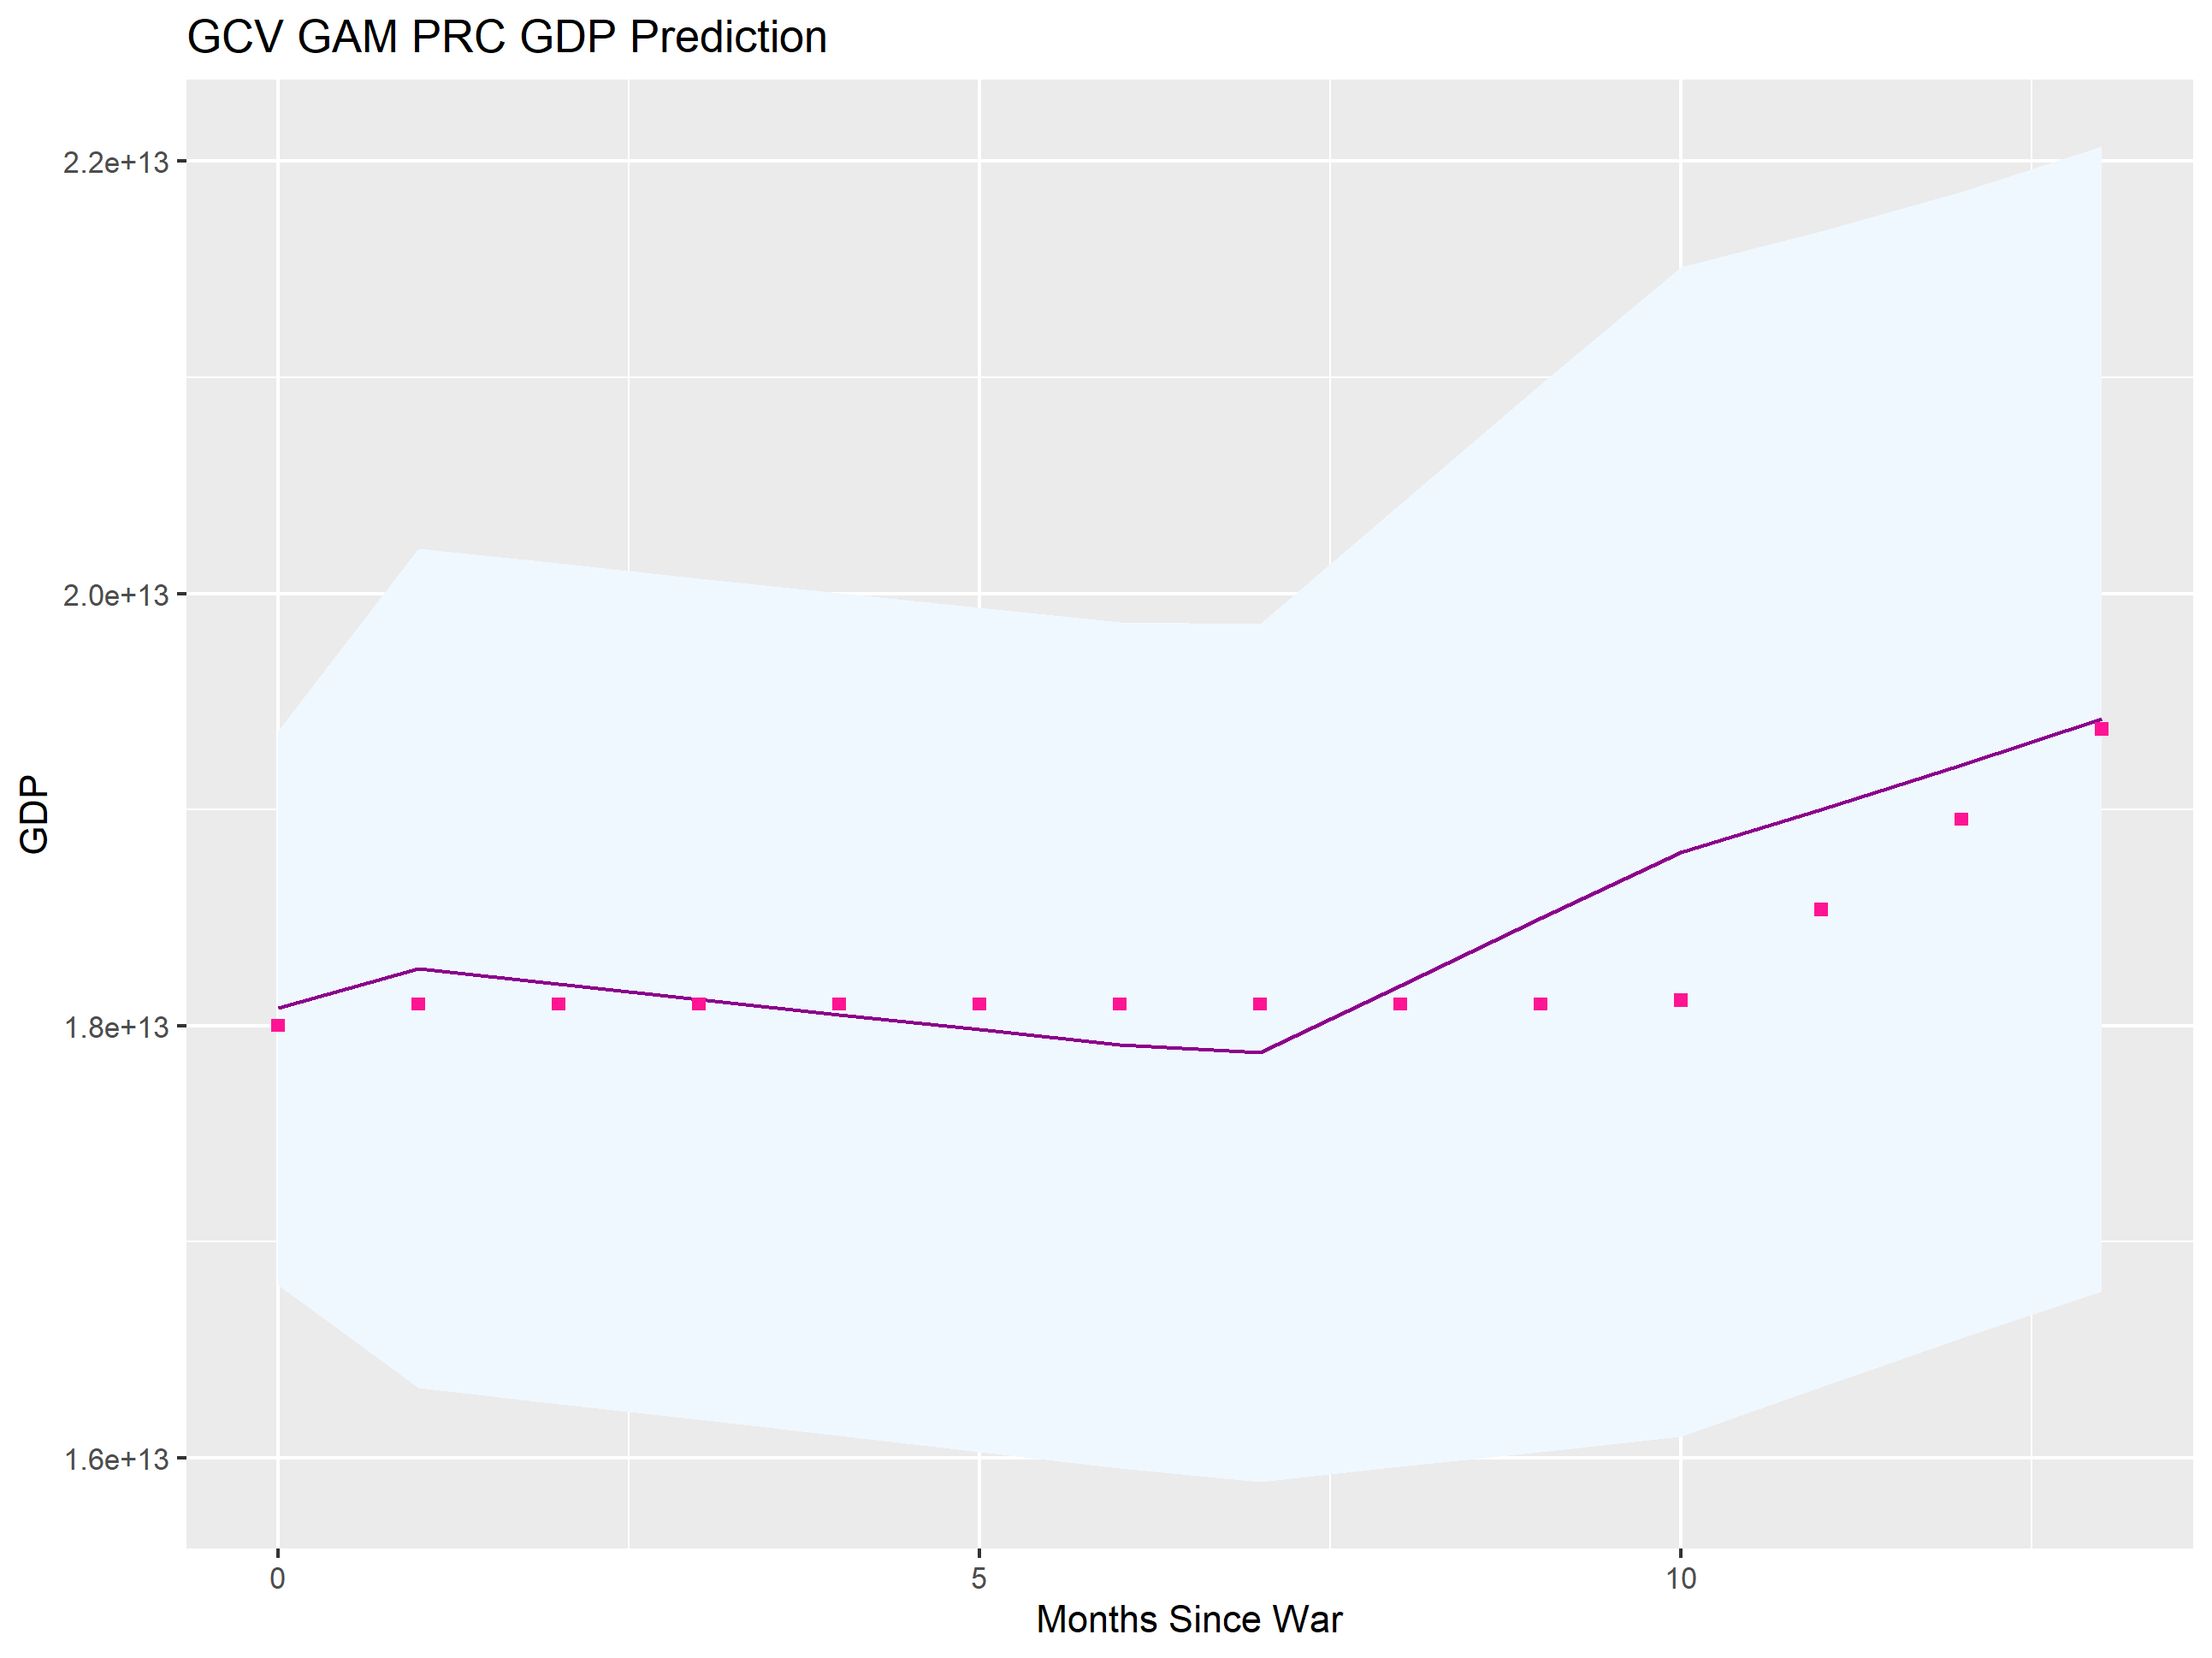
\includegraphics[width=2.2in]{report/prc-gdp-gcv.png}}  \quad
\subfigure{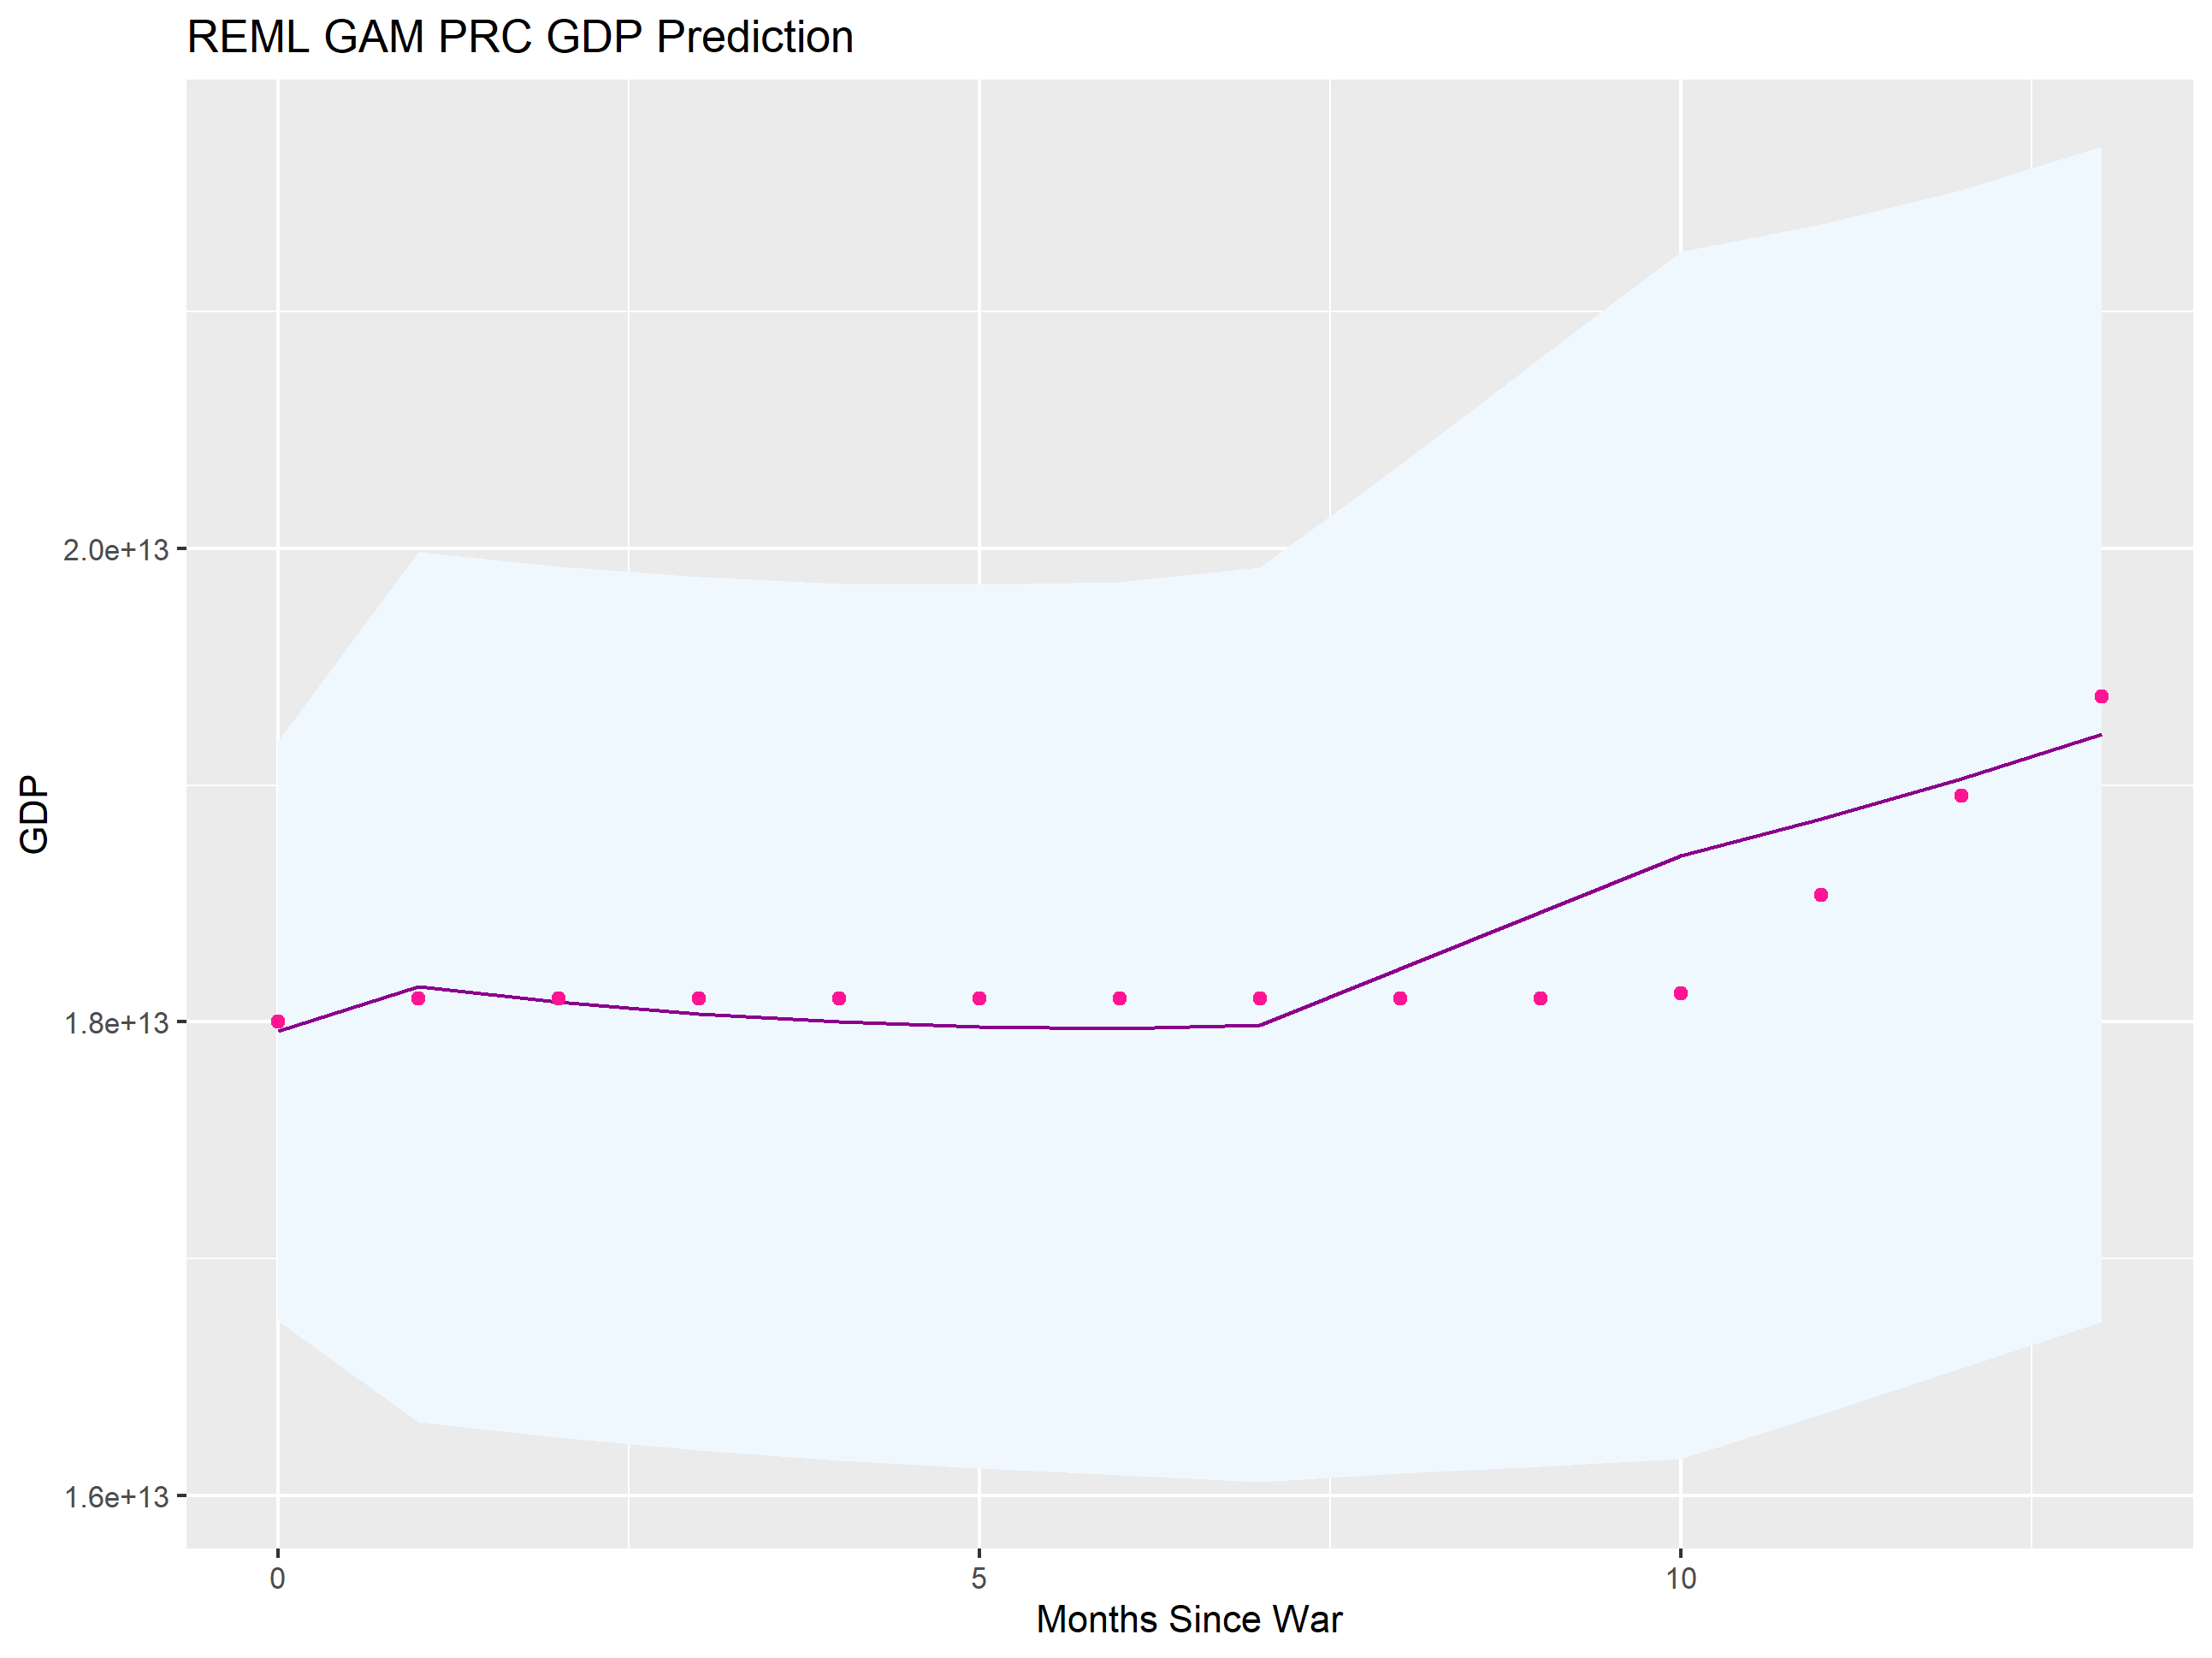
\includegraphics[width=2.2in]{prc-gdp-reml.png}}
}}
\caption{GAM models forecasts of GDP for the People's Republic of China using GCV and REML methods, with true observation values represented by the pink dots.}
\end{figure}

\begin{figure}
\centering
\centerline{ \mbox{
\subfigure{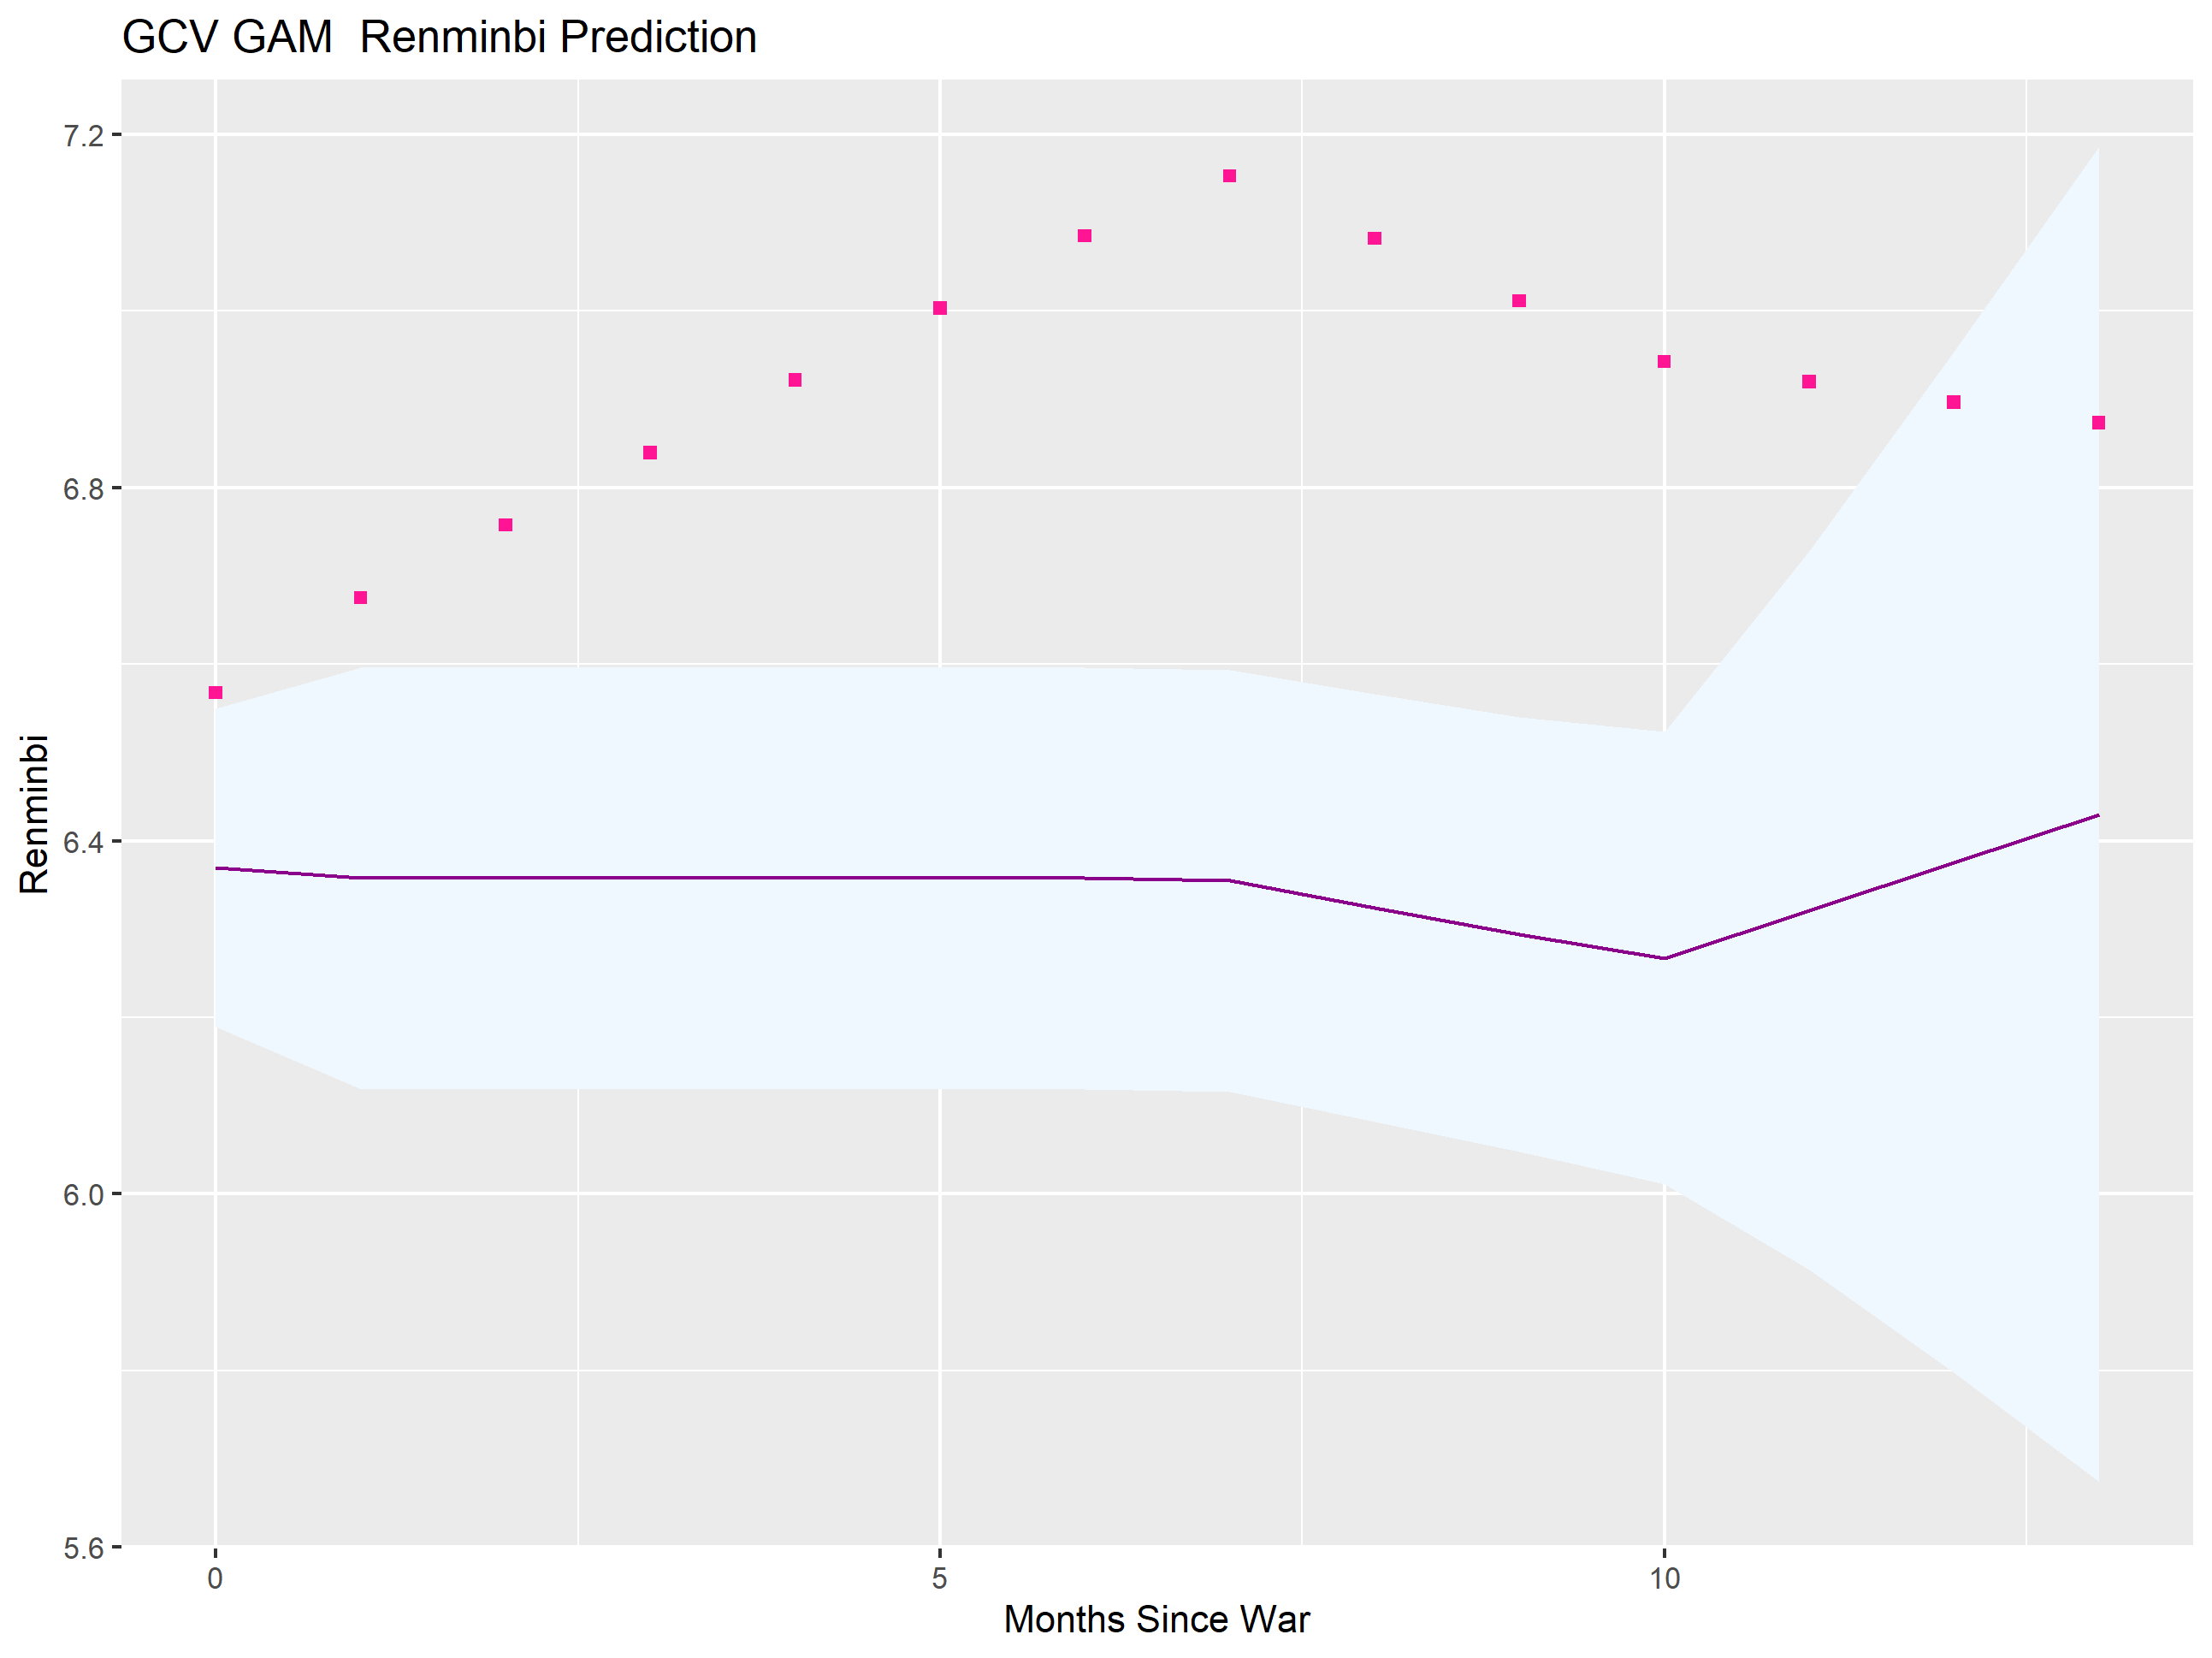
\includegraphics[width=2.2in]{report/prc-coin-gcv.png}}  \quad
\subfigure{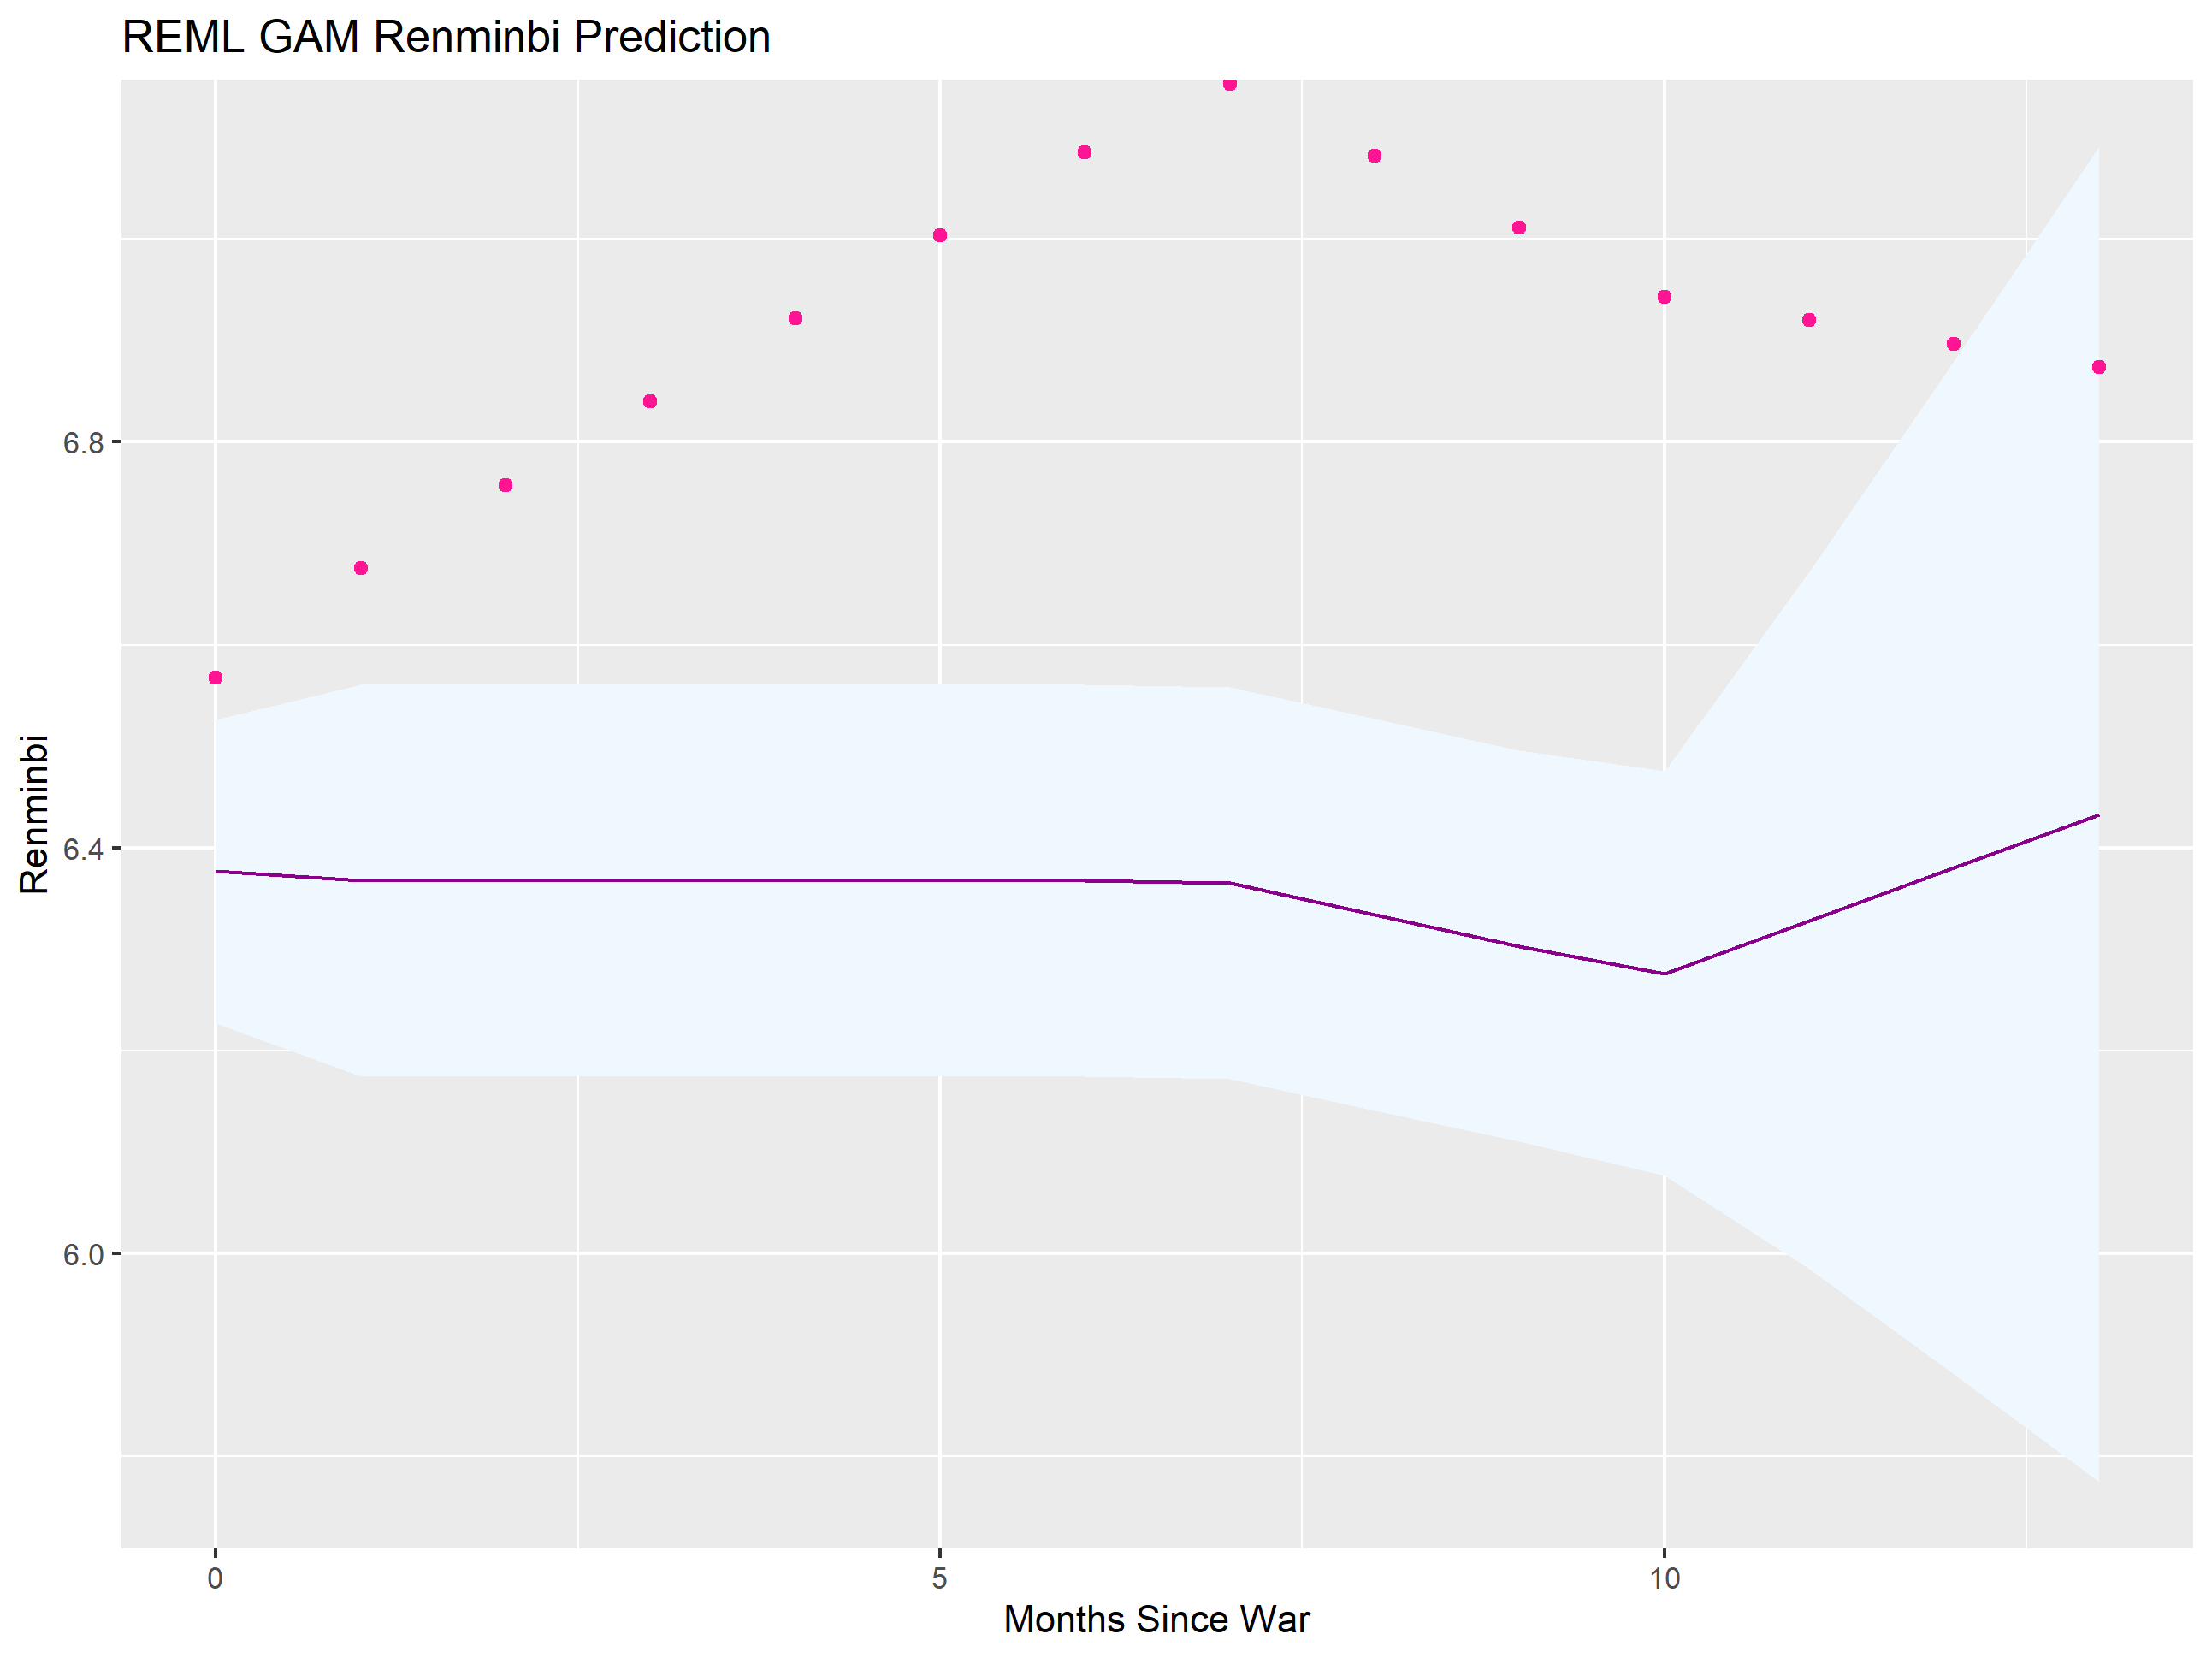
\includegraphics[width=2.2in]{report/prc-coin-reml.png}}
}}
\caption{GAM models forecasts of the Renminbi for the People's Republic of China using GCV and REML methods, with true observation values represented by the pink dots.}
\end{figure}


% GAM Summaries

\begin{figure}[h!]  
\caption*{\textit{Table 3:} USA Pre-war results regarding explained GCV and REML percentages, along with the accompanying dependent and independent variables}
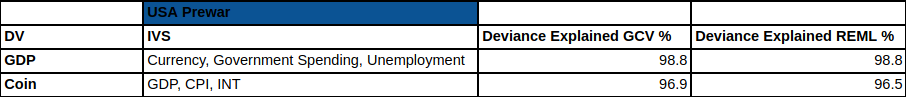
\includegraphics[width=6in]{usa_prewar_gam_summary.png}
\end{figure}

\begin{figure}[h!]  
\caption*{\textit{Table 4:} European Union pre-war GAM results for currency and GDP responses and their associated Deviance Explained values as a percentage.}
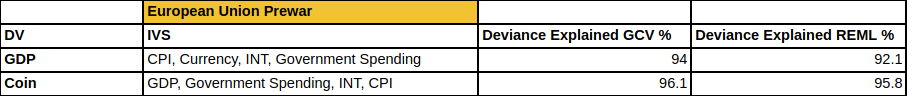
\includegraphics[width=6in]{eu_prewar_gam_summary.png}
\end{figure}

\begin{figure}[h!]  
\caption*{\textit{Table 5:} The PRC's Pre-war results regarding explained GCV and REML percentages, along with the accompanying dependent and independent variables}
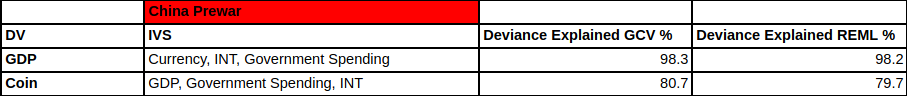
\includegraphics[width=6in]{china_prewar_gam_summary.png}
\end{figure}


\begin{figure}[h!]  
\caption*{\textit{Table 6:} Japan's pre-war GAM results for currency and GDP responses and their associated Deviance Explained values as a percentage.}
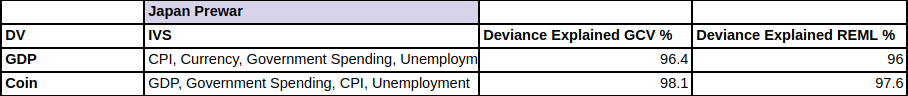
\includegraphics[width=6in]{japan_prewar_gam_summary.png}
\end{figure}
 % Please add the following required packages to your document preamble:
% \usepackage{multirow}
% \usepackage[table,xcdraw]{xcolor}
% If you use beamer only pass "xcolor=table" option, i.e. \documentclass[xcolor=table]{beamer}


\ 

\ 

\ 

\ 

\ 

\ 

\ 

\ 

\ 

\ 

\ 

\ 

\ 


\ 

\ 

\ 

\ 

\ 

\ 

\ 

\ 

\ 

\ 

\ 

\ 













\section*{Discussion and Conclusion}
To begin, we find many simultaneous significant independent variables in multiple models across each nation which are then able to reject our null hypothesis (1), as seen in Table 2.  Chiefly among these, we find the largest prevalence of rejected hypothesis predictors in that of Japan and the European Union, which might indicate these two have felt the largest impact since the war. The United States sees patterns by rejecting GDP and CPI in multiple models, where we interestingly see the effect of CPI on the Dollar transitioning from a negative coefficient to a positive one in pre-war and post-war eras. Among the European Union, we see particular trends in rejecting the Euro, CPI, Government Spending, and Interest Rates. Similarly Japan sees trends in the rejections of Government Spending, Unemployment Rate, and CPI across almost all models. Finally, the PRC has the least significant results, with only two predictors rejected among all six models, these being Government Spending and Interest Rates.

Comparing broadly among all datasets, we see the effect of CPI on GDP significantly changing in Japan, the United States, and the European Union. The change in regression coefficients for CPI on GDP in many of these cases is that of CPI increases in the post-war era being less positively correlated to a nation's rising GDP, which might imply the effects of the war have led to an increase in inflation while simultaneously not increasing the GDP by a large margin, as one would expect with such currency inflation. This could imply we are beginning to see the entry of a stagflationary cycle in the nations where we note this phenomenon- the USA, the European Union, and Japan. Another, less alarming, angle to see this could be a significant lag in the GDP growth catching up to inflationary trends.

Another significant trend observed in the three highly affected datasets (the EU, US, and Japan), is a broad trend of the GDP's effect on the national currency being statistically different in the pre-war and post-war eras. In Japan and the European Union, every instance of GDP affecting currency results in a transition to a higher positive effect on the currency itself. Since our Euro and Yen data is gauged in strength relative to the dollar, this could imply that these national currencies have gained in strength with their respective GDP while the value of the Dollar has weakened. Further supporting this, we see an opposite trend in the USA, with the GDP transitioning from a positive effect on the dollar to a negative effect.



With respect to Government spending, the economies of the European Union and Japan both see a similar transition from higher government spending leading to a positive effect (or lesser negative effect) on GDP to a highly negative effect in the post-war era. One possible explanation of this is these two respective entities are responding to the invasion by increasing their spending towards military aims, which can be seen from the recent efforts to re-militarize Japan \cite{japan_war} and European nations such as Poland reacting to the invasion by increasing the capacity of their armed forces \cite{poland}.  

Japan is the only nation which finds statistically significant differences with respect to the unemployment rate's effect on GDP. Each instance of rejection results in a shift from a negative effect to a positive effect or a less negative effect on GDP. One inference of this result could be that since unemployment rate has been relatively stable in the post-war era, any raise in GDP could be cancelling out the negative properties of a higher unemployment rate seen in the pre-war regressions. 

Curiously, we see few instances in any model across any nation where we can find a statistical difference with interest rates as a predictor. There are a few explanations for this, one being that many models were unable to use interest rates as an independent variable due to multicollinearity issues. In the cases where we do have a rejected hypothesis (Chinese GDP and EU Euro), we see the same result with an increase in interest rates affecting GDP less negatively in the post-war era. Here, we can summarize that interest rate increases in the European Union have less negatively effected the EU economy as previously seen with rate rises. The cause of this is not known at the time and should be studied further.

Additionally, the multiple regression models had relatively strong adjusted R-squared values. Across the board, the non-robust models have adjusted R-squared values ranging from around 0.4 to 0.98 across the pre-war and post-war models. The difference models have less strong adjusted R-squared values which might imply a faulty employment of such methods. Additional work can be down to analyze further if the difference models are properly implemented.

Regarding the GAM models, forecasting accuracy varies across each nation and the respective dependent variable. Overall, we see very similar forecasting results between GCV and REML methods with the exception of European Union forecasting results on GDP.

The United States shows very inaccurate forecasting results with respect to GDP under both methods, while Dollar forecasting results remain close to the fitted model and well in the confidence intervals. These inaccurate GDP forecasts might show that the post-war American GDP is exceeding expectations under less favorable macroeconomic conditions, while the dollar is relatively stable. 

European Union forecasts remain in the confidence intervals under the GCV method and straddle the bounds of the confidence intervals for the REML method. The reason for the inverted fit discrepancy seen in Figure 5 is unknown and deserves more analysis. The Euro is forecasted accurately by both models as seen in Figure 6. Similarly to the United States, one might infer that the Euro has remained stable since the invasion.

Both GDP and Yen forecasts are inaccurate. As the Japanese GDP has stayed essentially constant in the post-war era as seen in Figure 7 while other macroeconomic variables changed, it is reasonable to assume that the fitted forecast would be error prone. This is further supported by the previous acknowledgement of Japan having the highest rate of rejected predictors from Table 2. The results in Figure 8 implies the Yen is performing stronger than expected in light of the change in economic variables.

The forecasting results for Chinese GDP are accurate while the forecasting for the Renminbi has significant errors. Figure 10 shows that the fitted models expect a poorer performance of the Renminbi while in reality it has become more valuable.

Tables 3 through 6 show us the Deviance Explained from each GAM model, with values mostly very high between 92 percent and 98.8 percent for the European Union, Japan, and the United States. China shows less Deviance Explained with respect to the currency response models. This is suspected to be from the lack of data for China compared to the other nations.

For clarification, the $n$th “lag" in an autocorrelation plot refers to the amount of correlation that the $n$th term has to the current term in the time series. The ARIMAX results for the country GDP data were varied. In many cases, the partial autocorrelation functions of the GDP for the countries had its most significant lag above the 8 lag. In the case of the United States and the EU, this highly significant lag occurs at around the 13 mark. In the case of Japan and the PRC, this occurs at around the 8 or 9 lag mark. As this analysis was done in quarters, it could be said that at least for the United States and the European Union, this could be a byproduct of the COVID-19 epidemic's initial economic fallout around 13 quarters ago (Q1 of 2020). Besides that, none of the other lag terms were significant enough to lie outside of the 95\% confidence intervals highlighted in blue. The partial autocorrelation functions paint a different story, as there are terms that are the most significant as far as the 9th lag mark. These marks diminish steadily in size, with the first lag mark having the highest autocorrelation and the successive lag marks having less autocorrelation until lying within the marks of the confidence interval. With the European Union's autocorrelation function, the lags are a bit less significant earlier on, with the last significant lag being located at the 6th mark. 

This could perhaps be interpreted as there being less influence from previous states in the economy. To speculate as to why, it could be theorized that this could have to do with its relatively smaller economic size as opposed to the United State's economy. A similar effect occurs when comparing Japan and the PRC's economy. No stationarity was obtained by performing the Dickey-Fuller test with the different countries' GDP data. This likely reflects the seasonal nature of economies. For reference, a stationary time-series is one that has a constant mean, variance, and autocorrelation \cite{stationarity}. By simple inference, it is easy to see that most if not all economies do not exhibit stationarity. For that reason, the $d$ term is used to determine how many nonseasonal differences are required for stationarity. In the case of Japan, the United States, and Europe, a $d$ term of 3 was necessary, whereas a $d$ term of 2 was necessary for the PRC's data. If a differencing term is necessary for avoiding seasonality, then this implies that data which requires a higher $d$ term must be highly nonseasonal. In turn, this implies that the PRC's GDP data is less seasonal. This could be due to a number of reasons, some involving economic policies aimed at maintaining its high growth rate. However, when compared to the $d$ terms of the other countries, this could imply that perhaps the PRC's GDP conditions are more stable than those of the other countries.  

The results pertaining to the commodities offer a clearer picture. The time series data for all the commodities had a $d$ term of 2, which could indicate that these prices are less seasonal than the GDP data found above. The autocorrelation terms are commonly significant from the first term all the way to the 25th term, and it's likely that even more terms are significant. Given that the lag terms are in units of days, this likely reflects the fact that for a single month, the price of a commodity is highly related to its price at any other point in the past month. Another observation is that the partial autocorrelation terms for all the commodities are sparsely scattered, since virtually none of them rise above the significance level of 95\%. This suggests that autocorrelation is the main factor that affects current commodity futures prices, and not partial autocorrelation. As a result, very few of the attempted models utilized partial autocorrelation. 

For the ARIMA results regarding commodities, the results seem to indicate patterns that diverge from what is expected from the model. Technically, the patterns can be explained by the 95\% and 80\% confidence intervals of the ARIMA models, but overall, none of the observed patterns follow what the model predicts. This is particularly egregious with the wheat example, which was critically affected by the onset of the war and proceeded to diverge from the general trend by first undergoing a steep rise followed by a steep fall and a modest falloff. Some more subdued examples can be found in the Soybean Oil futures and Natural Gas futures.

Overall, we have established many possible effects on the economies the United States, European Union, China, and Japan as a result of the Russo-Ukrainian War through multiple regression and the forecasting methods of GAMs and autoregressive models. Additionally, while the ARIMAX results for the countries offer mixed results, with Europe showing the most drastic change from the model's expectations and Japan's results being expected,  the results of ARIMA modelling with regards to commidites offers a distinct change that occurs at the onset of the war. This in turn yields the clearest picture among all the autoregressive model results and clearly shows a change from the prewar conditions. Further work can expand on improved datasets, involving more nations, using more advanced regression techniques as well as utilizing neural network models to advance similar results.

While there is no absolute conclusion of a negative downturn across the global economy, we present significant results to illustrate that economic variables have shifted in light of a large scale war coming to Europe. 




\newpage





\section*{References}
\begingroup
\renewcommand{\section}[2]{}%
\begin{thebibliography}{9}


\bibitem{correct_stats}
Paternoster, R., Brame, R., Mazerolle, P., & Piquero, A. (1998). Using the correct statistical test for the equality of regression coefficients. Criminology, 36(4), 859-866.

\bibitem{GAM_business}
Sapra, S. K. (2013). Generalized additive models in business and economics. International Journal of Advanced Statistics and Probability, 1(3), 64-81.

\bibitem{economic_schock}
Miguel, E., Satyanath, S., & Sergenti, E. (2004). Economic Shocks and Civil Conflict: An Instrumental Variables Approach. Journal of Political Economy, 112(4), 725–753. https://doi.org/10.1086/421174

\bibitem{macroeconomic_mult_linreg}
Book, E., & Ekelöf, L. (2019). A Multiple Linear Regression Model To Assess The Effects of Macroeconomic Factors On Small and Medium-Sized Enterprises.


\bibitem{economic_civil_war}
Imai, K., & Weinstein, J. M. (2000). Measuring the economic impact of civil war. CID Working Paper Series.

\bibitem{linear_regression_economics}
Bazen, S. (2011). The use of linear regression in labour economics. Econometric Methods for Labour Economics, 4–33. https://doi.org/10.1093/acprof:oso/9780199576791.003.0002 




\bibitem{cinco}
A. Colin Cameron and Pravin K. Trivedi (2013), Regression Analysis of Count Data, 2nd edition,
Econometric Society Monograph No.53, Cambridge University Press, 1998 (566 pages.)

\bibitem{book}
Gelman A, Hill J., and Vehtari A. (2020)  Regression and Other Stories, Cambridge University Press

\bibitem{time_series_models}
Smelser, N. J., & Baltes, P. B. (2001, November). Time Series: Economic forecasting - harvard university. Retrieved April 29, 2023, from https://scholar.harvard.edu/files/stock/files/time\_series\_economic\_forecasting.pdf

\bibitem{ARIMA_forecasting}
Siami-Namini, S., & Siami Namin, A. (n.d.). Forecasting economics and financial time series: Arima vs. LSTM. Retrieved April 29, 2023, from https://ui.adsabs.harvard.edu/abs/2018arXiv180306386S/abstract

\bibitem{ARIMA_original} 
Box, G. E., Jenkins, G. M., Reinsel, G. C., & Ljung, G. M. (2015). Time series analysis: forecasting and control. John Wiley & Sons.

\bibitem{Thailand_ARIMAX}
Kongcharoen, C., & Kruangpradit, T. (2013, June). Autoregressive integrated moving average with explanatory variable (ARIMAX) model for Thailand export. In 33rd International Symposium on Forecasting, South Korea (pp. 1-8).

\bibitem{US-China-ARIMAX}
Rahmayanti, I., Andreas, C., & Ulyah, S. (2021). Does US-China trade war affect the Brent crude oil price? An ARIMAX forecasting approach. AIP Conference Proceedings, 2329(1).

\bibitem{irish-civil-war-ARIMAX} 
Mugtaba Osman, Andrew Parnell, & MacDara McCauley (2018). Effect of the Irish Civil War 1922-1923on suicide rates in Ireland: a retrospectiveinvestigation of the archives of the registrar general for Saorstat \'Eireann. Epidemiology Biostatistics and Public Health, 15(3), e12920.


\bibitem{Wheat_Ukraine}
Wheat in Ukraine. (n.d.). Retrieved April 29, 2023, from https://oec.world/en/profile/bilateral-product/wheat/reporter/ukr

\bibitem{Dickey-Fuller} 
 S. E. Said and D. A. Dickey (1984): Testing for Unit Roots in Autoregressive-Moving Average Models of Unknown Order. Biometrika 71, 599–607. 


\bibitem{stationarity}
Fuqua School of Business. (n.d.). Stationarity and differencing of time series data. https://people.duke.edu/~rnau/411diff.htm

\bibitem{subafrica}
Miguel, E., Satyanath, S., & Sergenti, E. (2004). Economic shocks and civil conflict: An instrumental variables approach. Journal of political Economy, 112(4), 725-753.

\bibitem{european_bank}
Chupilkin, M., & Koczan, Z. (2022). The Economic Consequences of War: Estimates Using Synthetic Controls. European Bank for Reconstruction and Development.

\bibitem{Glick}
Glick, R., & Taylor, A. M. (2010). Collateral damage: Trade disruption and the economic impact of war. The Review of Economics and Statistics, 92(1), 102-127.

\bibitem{poland}
Osborn, K. (2022, January 18). The Russian threat is behind Poland's F-35 purchase. Retrieved April 29, 2023, from https://nationalinterest.org/blog/buzz/russian-threat-behind-polands-f-35-purchase-199587

\bibitem{japan_war}
Li, R. (n.d.). The Remilitarization of Japan: An Uncertain Future. Retrieved April 29, 2023, from https://cs.wellesley.edu/~lianka110/beta/article1.html

\bibitem{GAM_wood}
Wood, S. N. (2006). Generalized Additive Models: An Introduction with R. Chapman and Hall/CRC.

\bibitem{RobustRegression}
Ruckstuhl, A. (2016). Robust Fitting of Parametric Models Based on M-Estimation.

\bibitem{Huber}
P. J. Huber (1981) Robust Statistics. Wiley.

\end{thebibliography}
\endgroup

\

\

\

\end{document}
